%%%%%%%%%%%%%%%%%%%%%%
\documentclass{amsart}
% !TEX root = ../ac_paper.tex

% General packages
\usepackage{microtype}
\usepackage{amsmath, amssymb, amsthm}
\usepackage{mathtools}
\usepackage{tikz-cd}
\usepackage{mathbbol} % changes \mathbb{} and adds more support

% Complex configurations
% bibliography
\usepackage[
backend=biber,
style=alphabetic,
backref=true,
url=false,
doi=false,
isbn=false,
eprint=false]{biblatex}

\renewbibmacro{in:}{} % don't display "in:" before the journal name
\AtEveryBibitem{\clearfield{pages}} % don't show page numbers

\DeclareFieldFormat{title}{\myhref{\mkbibemph{#1}}}
\DeclareFieldFormat
[article,inbook,incollection,inproceedings,patent,thesis,unpublished]
{title}{\myhref{\mkbibquote{#1\isdot}}}

\newcommand{\doiorurl}{%
	\iffieldundef{url}
	{\iffieldundef{eprint}
		{}
		{http://arxiv.org/abs/\strfield{eprint}}}
	{\strfield{url}}%
}

\newcommand{\myhref}[1]{%
	\ifboolexpr{%
		test {\ifhyperref}
		and
		not test {\iftoggle{bbx:eprint}}
		and
		not test {\iftoggle{bbx:url}}
	}
	{\href{\doiorurl}{#1}}
	{#1}%
}
 % bibliography management
% hyper-references
\usepackage[
bookmarks=true,
linktocpage=true,
bookmarksnumbered=true,
breaklinks=true,
pdfstartview=FitH,
hyperfigures=false,
plainpages=false,
naturalnames=true,
colorlinks=true,
pagebackref=false,
pdfpagelabels]{hyperref}

\hypersetup{
	colorlinks,
	citecolor=blue,
	filecolor=blue,
	linkcolor=blue,
	urlcolor=blue
}

% cross-references
\usepackage[capitalize, noabbrev]{cleveref} % hyper- and cross-referencing 

% Update to MSC2020
\makeatletter
\@namedef{subjclassname@2020}{%
	\textup{2020} Mathematics Subject Classification}
\makeatother

% Table of contents
\setcounter{tocdepth}{2}
% environments
\newtheorem{theorem}{Theorem}
\newtheorem*{theorem*}{Theorem}
\newtheorem{proposition}[theorem]{Proposition}
\newtheorem*{proposition*}{Proposition}
\newtheorem{lemma}[theorem]{Lemma}
\newtheorem*{lemma*}{Lemma}
\newtheorem{corollary}[theorem]{Corollary}
\newtheorem*{corollary*}{Corollary}
\theoremstyle{definition}
\newtheorem{definition}[theorem]{Definition}
\newtheorem*{definition*}{Definition}
\newtheorem{remark}[theorem]{Remark}
\newtheorem*{remark*}{Remark}
\newtheorem{example}[theorem]{Example}
\newtheorem*{example*}{Example}
\newtheorem{construction}[theorem]{Construction}
\newtheorem*{construction*}{Construction}
\newtheorem{convention}[theorem]{Convention}
\newtheorem*{convention*}{Convention}
\newtheorem{terminology}[theorem]{Terminology}
\newtheorem*{terminology*}{Terminology}
\newtheorem{notation}[theorem]{Notation}
\newtheorem*{notation*}{Notation}
\newtheorem{question}[theorem]{Question}
\newtheorem*{question*}{Question}

% hyphenation
\hyphenation{co-chain}
\hyphenation{co-chains}
\hyphenation{co-al-ge-bra}
\hyphenation{co-al-ge-bras}
\hyphenation{co-bound-ary}
\hyphenation{co-bound-aries}
\hyphenation{Func-to-rial-i-ty}
\hyphenation{colim-it}
\hyphenation{di-men-sional}

% basics
\DeclareMathOperator{\face}{d}
\DeclareMathOperator{\dege}{s}
\DeclareMathOperator{\bd}{\partial}
\DeclareMathOperator{\sign}{sign}
\newcommand{\ot}{\otimes}
\DeclareMathOperator{\EZ}{EZ}
\DeclareMathOperator{\AW}{AW}

% sets and spaces
\newcommand{\N}{\mathbb{N}}
\newcommand{\Z}{\mathbb{Z}}
\newcommand{\Q}{\mathbb{Q}}
\newcommand{\R}{\mathbb{R}}
\renewcommand{\k}{\Bbbk}
\newcommand{\sym}{\mathbb{S}}
\newcommand{\cyc}{\mathbb{C}}
\newcommand{\Ftwo}{{\mathbb{F}_2}}
\newcommand{\Fp}{{\mathbb{F}_p}}
\newcommand{\Cp}{{\cyc_p}}
\newcommand{\gsimplex}{\mathbb{\Delta}}
\newcommand{\gcube}{\mathbb{I}}

% categories
\newcommand{\Cat}{\mathsf{Cat}}
\newcommand{\Fun}{\mathsf{Fun}}
\newcommand{\Set}{\mathsf{Set}}
\newcommand{\Top}{\mathsf{Top}}
\newcommand{\CW}{\mathsf{CW}}
\newcommand{\Ch}{\mathsf{Ch}}
\newcommand{\simplex}{\triangle}
\newcommand{\sSet}{\mathsf{sSet}}
\newcommand{\cube}{\square}
\newcommand{\cSet}{\mathsf{cSet}}
\newcommand{\Alg}{\mathsf{Alg}}
\newcommand{\coAlg}{\mathsf{coAlg}}
\newcommand{\biAlg}{\mathsf{biAlg}}
\newcommand{\sGrp}{\mathsf{sGrp}}
\newcommand{\Mon}{\mathsf{Mon}}
\newcommand{\symMod}{\mathsf{Mod}_{\sym}}
\newcommand{\symBimod}{\mathsf{biMod}_{\sym}}
\newcommand{\operads}{\mathsf{Oper}}
\newcommand{\props}{\mathsf{Prop}}

% operators
\DeclareMathOperator{\free}{F}
\DeclareMathOperator{\forget}{U}
\DeclareMathOperator{\yoneda}{\mathcal{Y}}
\DeclareMathOperator{\Sing}{Sing}
\newcommand{\loops}{\Omega}
\DeclareMathOperator{\cobar}{\mathbf{\Omega}}
\DeclareMathOperator{\proj}{\pi}
\DeclareMathOperator{\incl}{\iota}
\DeclareMathOperator{\Sq}{Sq}
\DeclareMathOperator{\ind}{ind}

% chains
\DeclareMathOperator{\chains}{N}
\DeclareMathOperator{\cochains}{N^{\vee}}
\DeclareMathOperator{\gchains}{C}

% pair delimiters (mathtools)
\DeclarePairedDelimiter\bars{\lvert}{\rvert}
\DeclarePairedDelimiter\norm{\lVert}{\rVert}
\DeclarePairedDelimiter\angles{\langle}{\rangle}
\DeclarePairedDelimiter\set{\{}{\}}
\DeclarePairedDelimiter\ceil{\lceil}{\rceil}
\DeclarePairedDelimiter\floor{\lfloor}{\rfloor}

% other
\newcommand{\id}{\mathsf{id}}
\renewcommand{\th}{\mathrm{th}}
\newcommand{\op}{\mathrm{op}}
\DeclareMathOperator*{\colim}{colim}
\DeclareMathOperator{\coker}{coker}
\newcommand{\Hom}{\mathrm{Hom}}
\newcommand{\End}{\mathrm{End}}
\newcommand{\coEnd}{\mathrm{coEnd}}
\newcommand{\xla}[1]{\xleftarrow{#1}}
\newcommand{\xra}[1]{\xrightarrow{#1}}
\newcommand{\defeq}{\stackrel{\mathrm{def}}{=}}

% comments
\newcommand{\TBW}{\noindent TBW}

% pdf
\newcommand{\pdfEinfty}{\texorpdfstring{${E_\infty}$}{E-infty}}

% mathrm
\newcommand{\rA}{\mathrm{A}}
\newcommand{\rB}{\mathrm{B}}
\newcommand{\rC}{\mathrm{C}}
\newcommand{\rD}{\mathrm{D}}
\newcommand{\rE}{\mathrm{E}}
\newcommand{\rF}{\mathrm{F}}
\newcommand{\rG}{\mathrm{G}}
\newcommand{\rH}{\mathrm{H}}
\newcommand{\rI}{\mathrm{I}}
\newcommand{\rJ}{\mathrm{J}}
\newcommand{\rK}{\mathrm{K}}
\newcommand{\rL}{\mathrm{L}}
\newcommand{\rM}{\mathrm{M}}
\newcommand{\rN}{\mathrm{N}}
\newcommand{\rO}{\mathrm{O}}
\newcommand{\rP}{\mathrm{P}}
\newcommand{\rQ}{\mathrm{Q}}
\newcommand{\rR}{\mathrm{R}}
\newcommand{\rS}{\mathrm{S}}
\newcommand{\rT}{\mathrm{T}}
\newcommand{\rU}{\mathrm{U}}
\newcommand{\rV}{\mathrm{V}}
\newcommand{\rW}{\mathrm{W}}
\newcommand{\rX}{\mathrm{X}}
\newcommand{\rY}{\mathrm{Y}}
\newcommand{\rZ}{\mathrm{Z}}
% mathcal
\newcommand{\cA}{\mathcal{A}}
\newcommand{\cB}{\mathcal{B}}
\newcommand{\cC}{\mathcal{C}}
\newcommand{\cD}{\mathcal{D}}
\newcommand{\cE}{\mathcal{E}}
\newcommand{\cF}{\mathcal{F}}
\newcommand{\cG}{\mathcal{G}}
\newcommand{\cH}{\mathcal{H}}
\newcommand{\cI}{\mathcal{I}}
\newcommand{\cJ}{\mathcal{J}}
\newcommand{\cK}{\mathcal{K}}
\newcommand{\cL}{\mathcal{L}}
\newcommand{\cM}{\mathcal{M}}
\newcommand{\cN}{\mathcal{N}}
\newcommand{\cO}{\mathcal{O}}
\newcommand{\cP}{\mathcal{P}}
\newcommand{\cQ}{\mathcal{Q}}
\newcommand{\cR}{\mathcal{R}}
\newcommand{\cS}{\mathcal{S}}
\newcommand{\cT}{\mathcal{T}}
\newcommand{\cU}{\mathcal{U}}
\newcommand{\cV}{\mathcal{V}}
\newcommand{\cW}{\mathcal{W}}
\newcommand{\cX}{\mathcal{X}}
\newcommand{\cY}{\mathcal{Y}}
\newcommand{\cZ}{\mathcal{Z}}
% mathsf
\newcommand{\sA}{\mathsf{A}}
\newcommand{\sB}{\mathsf{B}}
\newcommand{\sC}{\mathsf{C}}
\newcommand{\sD}{\mathsf{D}}
\newcommand{\sE}{\mathsf{E}}
\newcommand{\sF}{\mathsf{F}}
\newcommand{\sG}{\mathsf{G}}
\newcommand{\sH}{\mathsf{H}}
\newcommand{\sI}{\mathsf{I}}
\newcommand{\sJ}{\mathsf{J}}
\newcommand{\sK}{\mathsf{K}}
\newcommand{\sL}{\mathsf{L}}
\newcommand{\sM}{\mathsf{M}}
\newcommand{\sN}{\mathsf{N}}
\newcommand{\sO}{\mathsf{O}}
\newcommand{\sP}{\mathsf{P}}
\newcommand{\sQ}{\mathsf{Q}}
\newcommand{\sR}{\mathsf{R}}
\newcommand{\sS}{\mathsf{S}}
\newcommand{\sT}{\mathsf{T}}
\newcommand{\sU}{\mathsf{U}}
\newcommand{\sV}{\mathsf{V}}
\newcommand{\sW}{\mathsf{W}}
\newcommand{\sX}{\mathsf{X}}
\newcommand{\sY}{\mathsf{Y}}
\newcommand{\sZ}{\mathsf{Z}}
% mathbb
\newcommand{\bA}{\mathbb{A}}
\newcommand{\bB}{\mathbb{B}}
\newcommand{\bC}{\mathbb{C}}
\newcommand{\bD}{\mathbb{D}}
\newcommand{\bE}{\mathbb{E}}
\newcommand{\bF}{\mathbb{F}}
\newcommand{\bG}{\mathbb{G}}
\newcommand{\bH}{\mathbb{H}}
\newcommand{\bI}{\mathbb{I}}
\newcommand{\bJ}{\mathbb{J}}
\newcommand{\bK}{\mathbb{K}}
\newcommand{\bL}{\mathbb{L}}
\newcommand{\bM}{\mathbb{M}}
\newcommand{\bN}{\mathbb{N}}
\newcommand{\bO}{\mathbb{O}}
\newcommand{\bP}{\mathbb{P}}
\newcommand{\bQ}{\mathbb{Q}}
\newcommand{\bR}{\mathbb{R}}
\newcommand{\bS}{\mathbb{S}}
\newcommand{\bT}{\mathbb{T}}
\newcommand{\bU}{\mathbb{U}}
\newcommand{\bV}{\mathbb{V}}
\newcommand{\bW}{\mathbb{W}}
\newcommand{\bX}{\mathbb{X}}
\newcommand{\bY}{\mathbb{Y}}
\newcommand{\bZ}{\mathbb{Z}}
% mathfrak
\newcommand{\fA}{\mathfrak{A}}
\newcommand{\fB}{\mathfrak{B}}
\newcommand{\fC}{\mathfrak{C}}
\newcommand{\fD}{\mathfrak{D}}
\newcommand{\fE}{\mathfrak{E}}
\newcommand{\fF}{\mathfrak{F}}
\newcommand{\fG}{\mathfrak{G}}
\newcommand{\fH}{\mathfrak{H}}
\newcommand{\fI}{\mathfrak{I}}
\newcommand{\fJ}{\mathfrak{J}}
\newcommand{\fK}{\mathfrak{K}}
\newcommand{\fL}{\mathfrak{L}}
\newcommand{\fM}{\mathfrak{M}}
\newcommand{\fN}{\mathfrak{N}}
\newcommand{\fO}{\mathfrak{O}}
\newcommand{\fP}{\mathfrak{P}}
\newcommand{\fQ}{\mathfrak{Q}}
\newcommand{\fR}{\mathfrak{R}}
\newcommand{\fS}{\mathfrak{S}}
\newcommand{\fT}{\mathfrak{T}}
\newcommand{\fU}{\mathfrak{U}}
\newcommand{\fV}{\mathfrak{V}}
\newcommand{\fW}{\mathfrak{W}}
\newcommand{\fX}{\mathfrak{X}}
\newcommand{\fY}{\mathfrak{Y}}
\newcommand{\fZ}{\mathfrak{Z}}

%%%%%%%%%%%%%%%%%%%%%%
% !TEX root = ../ac_paper.tex

% Include adittional packages below
\usepackage{amsfonts}
\usepackage{graphicx}
\usepackage{xcolor}
\usepackage{enumitem}
\usepackage{caption}
\usepackage{subcaption}
\usepackage{algorithm}
\usepackage{algpseudocode} % add packages here
% !TEX root = ../ac_paper.tex

\newcommand{\anibal}[1]{\todo[A.\!]{#1}}
\newcommand{\lucas}[1]{\todo[L.\!]{#1}}
\newcommand{\shehper}[1]{\todo[Sh.\!]{#1}}
\DeclareMathOperator{\length}{length}
\DeclareMathOperator{\Hard}{Hard}
\DeclareMathOperator{\Isol}{Isol}
\DeclareMathOperator{\Filt}{Filt}
\DeclareMathOperator{\Conn}{Conn}
\newcommand{\fixme}[1]{{{\color{blue}{[#1]}}}}
\newcommand{\AK}{\text{AK}}
\newcommand{\MS}{\text{MS}}
\newcommand{\G}{\text{G}}
\newcommand{\C}{\mathbb C}
\newcommand{\dm}{d_{\text{model}}}
\newcommand{\nc}{n_{\text{context}}}
\newcommand{\dhead}{d_{\text{head}}}
\newcommand{\softmax}{\text{Softmax}}
\newcommand{\FFN}{\text{FFN}}
\newcommand{\LN}{\text{LN}}
%\newcommand{\algorithmautorefname}{Algorithm} % add commands here
\addbibresource{aux/bibliography.bib} % add references here

%%%%%%%%%%%%%%%%%%%%%%
\title[What makes math problems hard for RL]{What makes math problems hard for reinforcement learning: a case study}
% !TEX root = ../ac_paper.tex

%\author[A.~Medina-Mardones]{Anibal~M.~Medina-Mardones}
%\address{Department of Mathematics, Western University, Canada}
%\email{\href{anibal.medina.mardones@uwo.ca}{anibal.medina.mardones@uwo.ca}}

\date{\today}
\subjclass[2020]{68T09, 62R07, 55N31, 62R40}
\keywords{reinforcement learning, large language models, topological data analysis, automated reasoning, search algorithms}

\begin{document}
	\vspace*{1cm}
	\begin{center}
		\textsc{---PREPRINT---}
	\end{center}
	\vspace*{1cm}

	% !TEX root = ../ac_paper.tex

\begin{abstract}
    Using a long-standing conjecture from combinatorial group theory, we explore, from multiple angles, the challenges of finding rare instances carrying disproportionately high rewards. Based on lessons learned in the mathematical context defined by the Andrews--Curtis conjecture, we propose algorithmic improvements that can be relevant in other domains with ultra-sparse reward problems.
    In the course of this study, we also address several open mathematical questions. Specifically, we establish the AC-triviality of two potential counterexamples from the Miller--Schupp family (1991) and demonstrate the AC length reducibility of all but two presentations in the Akbulut--Kirby (infinite) family (1981).
\end{abstract}

% \begin{abstract}
% 	Using a long-standing conjecture from combinatorial group theory, we explore, from multiple angles, the challenges of finding rare instances carrying disproportionately high rewards. Based on lessons learned in the mathematical context defined by the Andrews--Curtis conjecture, we propose algorithmic improvements that can be relevant in other domains with ultra-sparse reward problems.
%     Although our case study can be formulated as a game, its shortest winning sequences are potentially $10^6$ or $10^9$ times longer than those encountered in chess.
%     In the course of our study, we establish the AC-equivalence or AC-triviality of several significant potential counterexamples, including those from the Miller--Schupp family (1991) and the examples proposed by Akbulut and Kirby (1981).
% 	%whose status escaped direct mathematical methods for decades.
% 	%whose status had resisted direct mathematical methods for decades.
% 	%whose status had resisted resolution through direct mathematical methods for decades.
% \end{abstract}
	\maketitle
	\tableofcontents
	% !TEX root = ../ac_paper.tex

\section{Introduction\label{sec:intro}}

\TBW

\subsection*{Outline}

This paper is structured as follows. In \autoref{sec:AC}, we review the Andrews--Curtis conjecture. In \autoref{sec:search}, we use classical search algorithms to study the presentations of Miller--Schupp series. We devise a greedy search algorithm and show that it performs significantly better than the breadth-first search algorithm widely used to study this problem in the literature. We discover that the previously-known shortest potential counterexample to the stable AC conjecture, i.e. $\AK(3)$, is in fact stably AC-trivial.

In \autoref{sec:rl}, we use reinforcement learning to search through the space of balanced presentations. Specifically, we focus on the Proximal Policy Optimization algorithm. We find that while this algorithm performs significantly better than breadth-first search, it does not outperform greedy search. (See \autoref{fig:performance}.)

In \autoref{sec:lm}, we use a decoder-only Transformer model to study the language structure of balanced presentations. We find that easy and hard presentations form their own clusters inside the embedding space of the Transformer model.

\begin{figure}
	\centering
	\begin{subfigure}[b]{0.5\textwidth}
		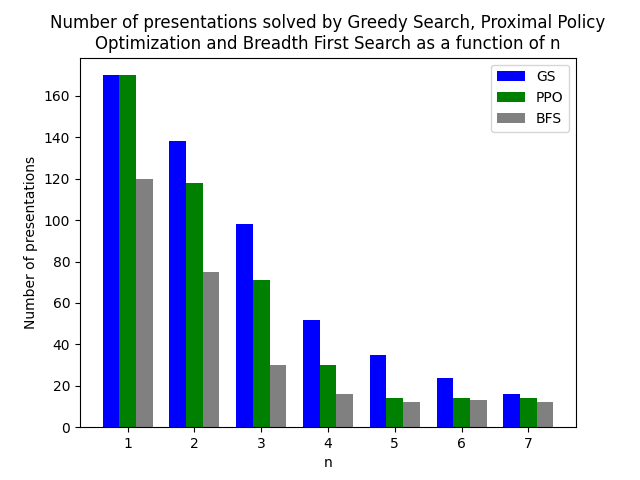
\includegraphics[width=1.1\textwidth]{fig/performance_vs_n.png}
		\caption{Distribution versus $n$}
		\label{fig:performance_vs_n}
	\end{subfigure}
	\begin{subfigure}[b]{0.5\textwidth}
		\centering
		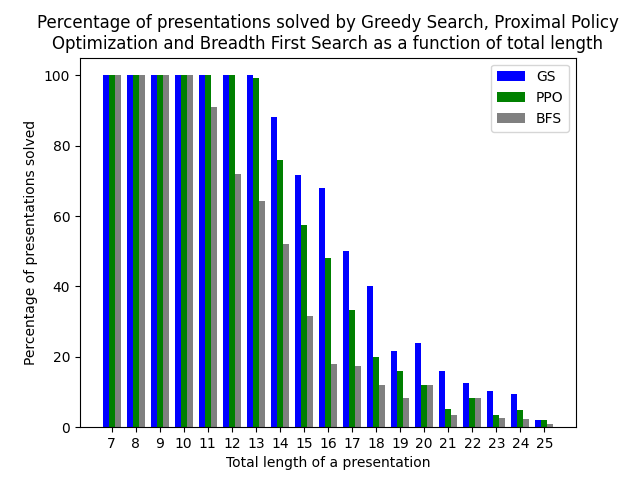
\includegraphics[width=1.1\textwidth]{fig/performance_vs_length.png}
		\caption{Distribution versus length}
		\label{fig:performance_vs_length}
	\end{subfigure}
	\caption{The figure shows a comparison of three algorithms --- breadth-first search, greedy search, and Proximal Policy Optimization (PPO) --- that we used to search through the space of balanced presentations. The number of presentations of the Miller--Schupp series, $\MS(n, w)$, solved by an algorithm is given on the vertical axis. We compare the performance as a function of $n$ (above) and the length of the presentation (below). Greedy Search consistently outperforms Breadth-First Search and Proximal Policy Optimization.}
	\label{fig:performance}\anibal{It would be better to include a PDF version of this pictures instead of a (compressed) PNG.}
\end{figure}

%We compare the performance of Greedy Search (GS), Breadth First Search and Proximal Policy Optimization on the presentations of Miller--Schupp series with $n, \ \length(w) \leq 7$ in \autoref{fig:performance}.

	% !TEX root = ../ac_paper.tex

\subsection*{Acknowledgment}

We would like to thank Anna Beliakova, Michael Douglas, Konstantin Korovin, Alexei Lisitsa, Maksymilian Manko, Ciprian Manolescu, Fabian Ruehle, Josef Urban, and Tony Yue Yu for insightful discussions and comments.

The work of S.G. is supported in part by a Simons Collaboration Grant on New Structures in Low-Dimensional Topology, by the NSF grant DMS-2245099, and by the U.S. Department of Energy, Office of Science, Office of High Energy Physics, under Award No. DE-SC0011632. The work of P.K. and B.L. is supported by the SONATA grant no. 2022/47/D/ST2/02058 funded by the Polish National Science Centre.
	% !TEX root = ../ac_paper.tex

\section{Andrews--Curtis conjecture\label{sec:AC}}

The Andrews--Curtis conjecture concerns the study of \textit{balanced presentations} of the trivial group, i.e.
presentations of the trivial group with an equal number of generators and relators.
The conjecture proposes that any balanced presentation
\[
\angles{x_1, \dots, x_n \mid r_1, \dots, r_n}
\]
can be converted to the trivial presentation
\[
\angles{x_1, \dots, x_n \mid x_1, \dots, x_n}
\]
through a series of the following operations known as \textit{AC moves} \cite{Andrews--Curtis}.
\begin{enumerate}[label=(AC\arabic*)]
	\item Substitute some $r_i$ by $r_i r_j$ for $i \neq j$.
	\item Replace some $r_i$ by $r_i^{-1}$.
	\item Change some $r_i$ to $g r_i g^{-1}$ where $g$ is a generator or its inverse.
\end{enumerate}
We will refer to the sum of the word lengths of all relators as the \textit{length} of a presentation, to two presentations related by a sequence of AC moves as \textit{AC-equivalent}, and to a presentation AC-equivalent to the trivial presentation as \textit{AC-trivial}.
Despite considerable efforts, little progress has been made in establishing a proof of the conjecture.
However, several families of potential counterexamples have been suggested in the literature.

To investigate a given presentation, one may systematically explore the entire space of possible sequences of AC moves in search of a sequence that renders the presentation trivial.
This space grows exponentially with the length of the sequence.
For a presentation with $n$ generators, there are $3n^2$ AC moves, and the total number of sequences of AC moves of length $k$ is $(3n^2)^k$.
Even for a modest case like $n=2$ and $k=20$, the number of possible sequences is on the order of $10^{21}$, making a brute-force approach impractical.
\newline

Classical search algorithms such as genetic algorithms \cite{genetic}, and breadth-first search \cite{bfs-ac} have been employed to search through this space and achieved success in trivializing balanced presentations with two generators and lengths less than 13.
The following presentation of length 13,
\[
\angles{x, y \mid x^3 = y^4, xyx = yxy}
\]
is the shortest presentation, up to AC-equivalence, that eludes all attempts at length reduction.
This presentation is a part of an infinite series of potential counterexamples by Akbulut and Kirby \cite{Akbulut--Kirby}:
\[
\AK(n) = \angles{x, y \mid x^n = y^{n+1}, xyx = yxy}, \quad n \geq 2.
\]
$\AK(2)$ has length 11 and has been established as AC-trivial \cite{genetic} whereas $\AK(3)$ is the aforementioned presentation with length 13.
\newline

In over two decades since the first utilization of search algorithms \cite{genetic, bfs-ac}, only unsuccessful attempts have been made to trivialize $\AK(3)$ with different variants of breadth-first search algorithm using an increased amount of computational resources \cite{Bowman-McCaul, krawiec2016distance, Panteleev-Ushakov}.
Notably, \cite{Panteleev-Ushakov} found that no sequence of AC moves that allows relator lengths to increase up to 20 trivializes $\AK(3)$.
This lack of success could be interpreted as suggestive evidence that $\AK(3)$ might be a counterexample to the Andrews--Curtis conjecture.
However, recent works by Bridson and Lishak have shown that there exist AC-trivializable balanced presentations of the trivial group, for which the number of AC moves in a trivializing sequence is bounded below by a superexponential function of the length of the presentation \cite{Bridson, Lishak}.
Roughly speaking, for these presentations, if the sum of word lengths is $k$, the number of AC moves required to trivialize the presentation is at least $\Delta (\lfloor \log_2 k \rfloor)$ where $\Delta \colon \mathbb{N} \to \mathbb{N}$ is defined recursively as $\Delta(0) = 2$ and $\Delta (j) = 2^{\Delta(j-1)}$ for $j \geq 1$.
In particular, $\Delta (\lfloor \log_2 (13) \rfloor) = 65536$, whereas presentations trivialized by the aforementioned search algorithms have AC sequences of length less than $1000$.
While $\AK(3)$ is itself not a member of the family of examples studied by Boris and Lishak, their findings challenge the inclination to view it as a counterexample.
Their work also underscores the necessity of employing search methods that are more efficient than breadth-first search.
\newline

In this paper, we will consider a variety of computational tools to better understand the properties of balanced presentations of the trivial group.
We will test the efficacy of our approaches on a subset of presentations from the Miller--Schupp series of potential counterexamples \cite{Miller--Schupp}.
\[
\MS(n, w) = \angles{x, y \mid x^{-1} y^n x = y^{n+1}, x = w}.
\]
Here, $n > 0$, and $w$ is a word in $x$ and $y$ with zero exponent sum on $x$.
For $w_\star = y^{-1} x^{-1} y x y$, the presentations $\MS(n, w_\star)$ are AC-equivalent to the presentations from Akbulut--Kirby series \cite{MMS}.
In particular, the presentation
\[
\MS(n, w) = \angles{x, y \mid x^{-1} y^3 x = y^{4}, x =  y^{-1} x^{-1} y x y}.
\]
of length 15 is AC-equivalent to $\AK(3)$.

We will only consider presentations with $n,\, \length(w) \leq 7$.
Our selection criteria aimed to strike a balance: we sought a dataset of presentations large enough to allow for meaningful analysis, yet small enough to ensure all computations are feasible within a practical timeframe.
Additionally, we reduced $x^{-1}w$ freely and cyclically and kept only one representative of each orbit under the action of cyclic permutations.\anibal{What is the action?}
After these simplifications, we were left with $170$ choices for $x^{-1} w$.
This resulted in a dataset of $7 \times 170 = 1190$ presentations from the Miller--Schupp series.
\newline

Our implementation of AC transformations differed from the AC transformations mentioned above in two ways.
First, we considered the following set of operations.
\begin{enumerate}[label=(AC$'$\arabic*)]
	\item Substitute some $r_i$ by $r_i r_j^{\pm 1}$ for $i \neq j$.
	\item Change some $r_i$ to $g r_i g^{-1}$ where $g$ is a generator or its inverse.
\end{enumerate}
For two generators, which is the only case we study in this paper, the group generated by these AC transformations is isomorphic to the group generated by the original AC transformations.\footnote{
The difference lies in how the inversion of a relator is handled: we always follow an inversion by a concatenation, while the original AC moves allow for standalone inversion moves.
The original inversion moves may be retrieved from the new generators as follows.
For a given presentation $\angles{x_1, x_2 \mid r_1, r_2}$, the sequence of moves: $r_2 \to r_2 r_1$, $r_1 \to r_1 r_2^{-1}$, $r_2 \to r_2 r_1$, and $r_2 \to r_1 r_2 r_1^{-1}$ results in the presentation $\angles{x_1, x_2 \mid r_2^{-1}, r_1}$, which is the same as $r_2 \to r_2^{-1}$ up to swapping the two relators.
We also enhanced the notion of trivial presentation(s) to include all presentations of length 2: $\{\angles{x_1, x_2 \mid x_i^{a}, x_j^{b}}  \mid i, j = 1, 2; a, b = \pm 1; i \neq j \}$.
}
The reason for this change is due to its effect on performance in greedy search and reinforcement learning algorithms studied in \autoref{sec:search} and \autoref{sec:rl}.
Specifically, the length of a presentation provides a useful signal when searching through the space of presentations with these algorithms.
An inversion transformation leaves the length invariant providing no signal to the search process and slowing down the performance of the algorithm significantly.
For the rest of the paper we will refer to the new transformations (instead of the original AC transformations) as ``AC transformations" or ``AC moves".

Second, in order to make the search space finite in size, we set a maximum length that each relator is allowed to take.
If an AC transformation resulted in a presentation with a relator of length greater than this maximum length, the AC transformation was set to act trivially.
In the search of a sequence of AC moves that trivialize a presentations of the Miller--Schupp series $\MS(n, w)$, we set this maximum length to be $2 \times \text{max}(2 n+3, \length(w)+1) + 2$.
This specific choice was made to allow for at least one concatenation move followed by a conjugation move in the search process.
%Note that this constraint is quite restrictive: any presentation of the Miller--Schupp series that requires the length of a relator to grow to more than the set maximum length would not be trivialized.

\subsection*{The Stable Andrews--Curtis Conjecture}\label{sec:stable_ac}

The Andrews--Curtis conjecture has many known variants.
\fixme{include references} We briefly explored one of these variants, namely the ``stable" or ``weak" Andrews--Curtis conjecture.
The stable version allows two more transformations in addition to the usual AC moves:.

\begin{enumerate}[label=(AC\arabic*)]
	\setcounter{enumi}{3}
	\item Include a new generator and a trivial relator, i.e. replace $\angles{x_1, \dots, x_n \mid r_1, \dots, r_n}$ by $\angles{x_1, \dots, x_n, x_{n+1} \mid r_1, \dots, r_n, x_{n+1}}$.
	\item Remove a trivial relator and the corresponding generator, i.e. the inverse of transformation (4).
\end{enumerate}
If two balanced presentations of the trivial group are related by a sequence of AC transformations (AC1) through (AC5), we say that they are \textit{stably AC-equivalent}.
The stable Andrews--Curtis conjecture states that any balanced presentation is stably AC-equivalent to the trivial presentation.
\newline

To the best of our knowledge, the shortest potential counterexample to the standard Andrews--Curtis conjecture, $\AK(3)$, was also believed to be a potential counterexample to the stable Andrews--Curtis conjecture before this work.
We show in \autoref{sec:search} that $\AK(3)$ is in fact stably AC-trivial.
Our proof builds on the following result.

\begin{theorem*}[Myasnikov, Myasnikov, and Shpilrain, \cite{MMS}]\label{theorem:MMS}
	Using the notation $[a, b] = a b a^{-1} b^{-1}$ and $[a, b, c] = [[a, b], c]$, any presentation of the following form is a presentation of the trivial group:
	\[
	\langle x, y, z \mid x = z \cdot [y^{-1}, x^{-1}, z], y = x \cdot [y^{-1}, x^{-1}, z^{-1}] \cdot [z^{-1}, x], w \rangle,
	\]
	where $w$ is a word in $x$, $y$, and $z$ whose exponent sum on $x$, $y$, and $z$ equals $\pm 1$.
\end{theorem*}

They obtained these presentations by applying Reidemeister moves to the knot diagram of the unknot.
Reidemeister moves applied to a knot diagram are known to give stably AC-equivalent Wirtinger presentations of the knot group.\anibal{Is there a reference?}
Thus the presentations in the theorem are all stably AC-trivial.

For $w = x^{-1}yz$, they reduced the presentation to the following length 25 presentation with two generators by eliminating $z$,
%\footnote{
%They used a computer program to further reduce this presentation to a length 14 presentation,
%\[
%\angles{x, y \mid x y x^{-2} = y x^{-1} y, xy^2 x = y x y}.
%\]
%We focus on the length 25 presentation as it follows clearly from the presentations in the theorem.
%}
\[
\angles{ x, y \mid
x^{-1}y^{-1}xy^{-1}x^{-1}yxy^{-2}xyx^{-1}y,
y^{-1}x^{-1}y^2x^{-1}y^{-1}xyxy^{-2}x }.
\]
We discovered a sequence of AC transformations that relates this presentation to $\AK(3)$.
(See \autoref{sec:stable_ak3} for this sequence of moves.)
This also makes $\AK(3)$ the shortest stably AC-trivial presentation that is not yet known to be AC-trivial.
\newline

It is plausible that by varying $w$ one can show that other presentations of the Akbulut--Kirby series (or the Miller--Schupp series) are also stably AC-trivial.
We leave this question for future work.
	% !TEX root = ../ac_paper.tex

\section{Classical search algorithms}\label{sec:search}

In this section, we compare the effectiveness of breadth-first and greedy search algorithms to AC-trivialize presentations in the Miller--Schupp series.
We find that the latter significantly outperforms the former. Based on our empirical observations, we find AC-triviality of infinite subfamilies of the Miller--Schupp series, as well as length reductions of $\AK(n)$. 

\subsection{Breadth-first search}

In breadth-first search (See \cref{alg:bfs} for pseudocode), we start with an initial state, which is a balanced presentation we aim to AC-trivialize, and place it in a queue. At each iteration, a state is removed from the queue, and its neighbors are added if they have not already been visited. This process continues until the sought-after state, i.e., a trivial balanced presentation, is found or a maximum number of states $N$ is visited. In our experiments, we set $N = 10^6$.

\begin{algorithm}
	\caption{Breadth-First Search}\label{alg:bfs}
	\begin{algorithmic}[1] % The number [1] ensures lines are numbered
		\State \textbf{Input:} A balanced presentation $\pi$, maximum number of states to visit $N$
		\State \textbf{Output:} Boolean for whether an AC trivialization is found
		\State Initialize a queue $Q$ and enqueue the starting node $\pi$
		\State Mark $\pi$ as visited
		\While{Number of visited states is less than $N$}
		\State $u \gets Q$.dequeue() \Comment{Remove the front node of $Q$}
		\For{each neighbor $v$ of $u$}
		\If{$v$ is a trivial state}
		\State \Return True \Comment{Return True if $v$ is a trivial state}
		\EndIf
		\If{$v$ has not been visited}
		\State Mark $v$ as visited
		\State $Q$.enqueue($v$) \Comment{Add $v$ to the queue}
		\EndIf
		\EndFor
		\EndWhile
		\State \Return False \Comment{Return False if no trivial state is found}
	\end{algorithmic}
\end{algorithm}

\subsection{Greedy search}\label{ss:greedy_search}

Greedy search, described in \cref{alg:gs}, differs only slightly from breadth-first search. We replace the queue with a priority queue, which stores the states in order determined by a tuple of values $(k, l)$, where $k$ is the length of the presentation and $l$ is the path length between the state and the initial state.

Instead of dequeuing the earliest state, the algorithm dequeues the state with the smallest value of $k$. If there is more than one state in the priority queue with the same value of $k$, the state with the smallest value of $l$ is chosen.

\begin{algorithm}
	\caption{Greedy Search}\label{alg:gs}
	\begin{algorithmic}[1] % The number [1] ensures lines are numbered
		\State \textbf{Input:} A balanced presentation $\pi$ of length $k$, maximum number of states to visit $N$
		\State \textbf{Output:} Boolean for whether an AC trivialization is found
		\State Initialize a \textit{priority} queue $Q$ ordered by $(k, l)$ and enqueue the starting node $\pi$.
		$l$ is the length of the path connecting $\pi$ to the current node.
		\State Mark $\pi$ as visited
		\While{Number of visited states is less than $N$}
		\State $u \gets Q$.dequeue() \Comment{Remove the front node of $Q$}
		\For{each neighbor $v$ of $u$}
		\If{$v$ is a trivial state}
		\State \Return True \Comment{Return True if $v$ is a trivial state}
		\EndIf
		\If{$v$ has not been visited}
		\State Mark $v$ as visited
		\State $Q$.enqueue($v$) \Comment{Add $v$ to the queue}
		\EndIf
		\EndFor
		\EndWhile
		\State \Return False \Comment{Return False if no trivial state is found}
	\end{algorithmic}
\end{algorithm}

\subsection{Comparison of performance on Miller--Schupp series}\label{sec:search-ms}

We find that greedy-search outperforms breadth-first search in the task of AC-trivializing Miller--Schupp presentations. %\cref{fig:performance}
Out of the 1190 presentations in the Miller--Schupp series with $n \leq 7$ and $\length(w) \leq 7$, greedy search solved 533 while BFS solved only 278.
Each algorithm was constrained to visit a maximum of 1 million nodes.
The percentage of presentations solved by these algorithms decreases monotonically as a function of $n$, with greedy search being able to solve all presentations with $n=1$ (see \cref{fig:performance_of_search_vs_n}).
This empirical result encouraged us to prove AC-triviality of the infinite family $\MS(1, w)$, which we give in \cref{sec:ms1w_}.

\begin{figure}
	\centering
    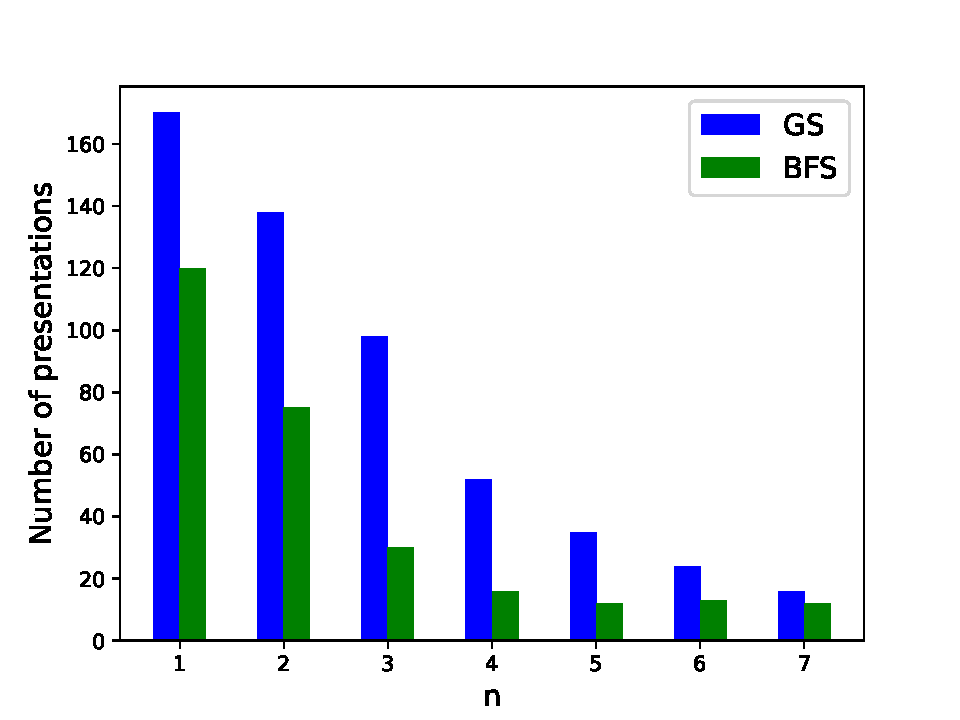
\includegraphics[width=0.6\textwidth]{fig/performance_of_search_vs_n.pdf}
    \caption{Comparison of greedy and breadth-first search algorithms as a function of $n$.
    The number of presentations of the Miller--Schupp series, $\MS(n, w)$, solved by an algorithm is given on the vertical axis.}
	\label{fig:performance_of_search_vs_n}
\end{figure}

Greedy search was also able to solve all presentations of length less than 14.
At length 14, there are six presentations that greedy search could not solve. We verified that four of these,
\[
\angles{x, y \mid x^{-1} y^2 x = y^{3} , x = x^{-2} y^{-1} x^2 y^{\pm 1}}
\]
\[
\angles{x, y \mid x^{-1} y^3 x = y^{4} , x = y^{\pm 1} x^2 y^{\pm 1}}
\]
are AC-equivalent to $\AK(3)$, while the other two
\[
\angles{x, y \mid x^{-1} y^2 x = y^{3} , x = y x^2 y^{\pm 1} x^{-2}}
\]
could be related neither to $\AK(3)$ nor to the trivial presentation through any path involving only presentations with both relators having length less than 20.

For presentations solved by greedy search, we plot the maximum amount by which the length of a presentation increased in an AC trivialization path in \cref{fig:gs_length_increase}.
In most cases, there was no increase in length; and the maximum increase was only~5.
At first glance, this seemed surprising to us, given that we allowed the relator lengths to increase by a much larger amount in our search process.\footnote{The length of each relator was allowed to increase up to \(2 \times \text{max}(2n+3, \length(w)+1) + 2\), which is twice the maximum of the initial lengths of the two relators in a presentation, plus an additional 2.
The maximum possible increase in presentation length is twice this number minus the original length.
For $n \leq 7$ and $\length(w) \leq 7$, this value lies in the range $[17, 53]$.}
However, the hard cutoff set by visiting a maximum of only 1 million nodes ensures that any presentation that needs to be mapped to a much longer presentation before it is trivialized would remain unsolved by the greedy search algorithm.
This limitation could be cured either by increasing the number of maximum nodes (at the cost of higher memory use) or by using a different criterion to order nodes in the priority queue.
It will be useful to explore the latter approach perhaps by looking for a criterion itself using deep learning algorithms.

We also plot the lengths of AC sequences discovered by greedy search as functions of $n$ and the maximum increase in the presentation length (\cref{fig:gs_path_length}).
Unsurprisingly, path lengths increase proportionally with the increase in the length of the presentation (\cref{fig:path_lengths_vs_length_increase}).
The following presentation with $n=5$ had the longest AC trivialization path,
\[
\angles{x, y \mid x^{-1} y^5 x = y^6,  x = y x^2 y^{-1}}
\] %correcting : \[\angles{x^{-1} y^5 x = y^6 \mid x = y x^2 y^{-1}}\]
requiring a sequence of 344 AC-moves.
Note that greedy search does not necessarily find the shortest paths of trivialization.
We will see in \cref{sec:application} that a Reinforcement Learning algorithm finds shorter trivializing sequences for many examples of the Miller--Schupp series.
This again hints at the potential utility of exploring more efficient criteria for ordering nodes in the priority queue.

In the remainder of this paper, we will refer to the presentations from the Miller--Schupp series that were solved and unsolved by the greedy search as ``GS-solved" and ``GS-unsolved" presentations, respectively. In other words, many of our experiments will be tested on two datasets that consists of Miller--Schupp presentations with $n \leq 7$ and $\length(w) \leq 7$: the GS-solved dataset has 533 presentations, whereas GS-unsolved dataset has 657 presentations. The combined dataset that contains all presentations with $n \leq 7$ and $\length(w) \leq 7$ has size 1190.

\begin{figure}
	\centering
	\begin{subfigure}[b]{0.5\textwidth}
		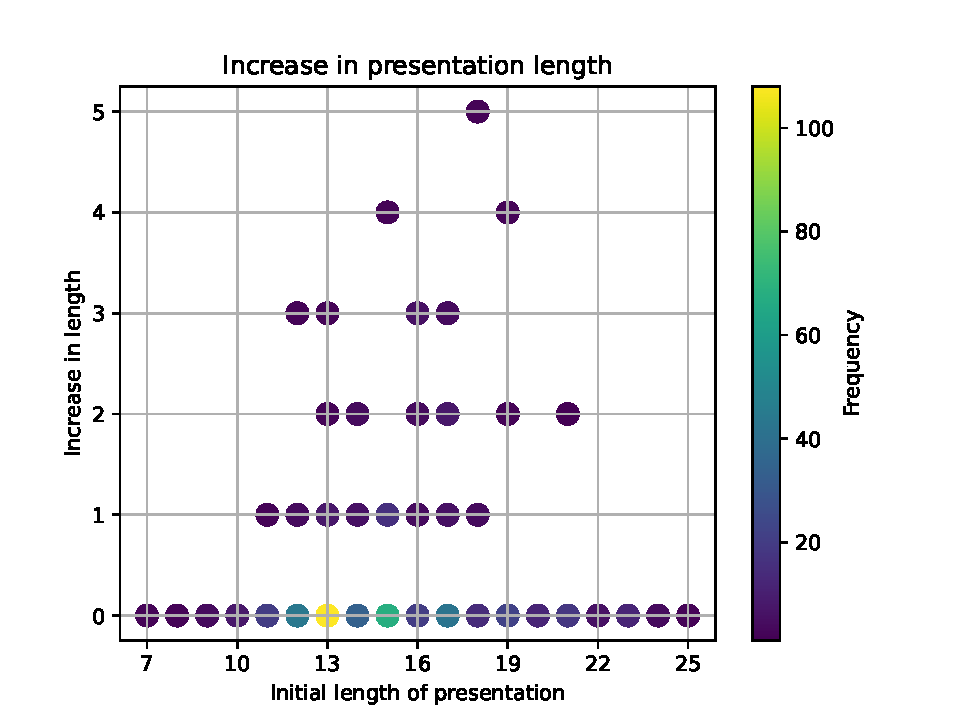
\includegraphics[width=\textwidth]{fig/gs_length_increase_vs_length.pdf}
		\caption{Distribution versus initial presentation length.}
		\label{fig:gs_length_increase_vs_length}
	\end{subfigure}%
	%add desired spacing between images, e. g. ~, \quad, \qquad etc.
	%(or a blank line to force the subfigure onto a new line)
	\begin{subfigure}[b]{0.5\textwidth}
		\centering
		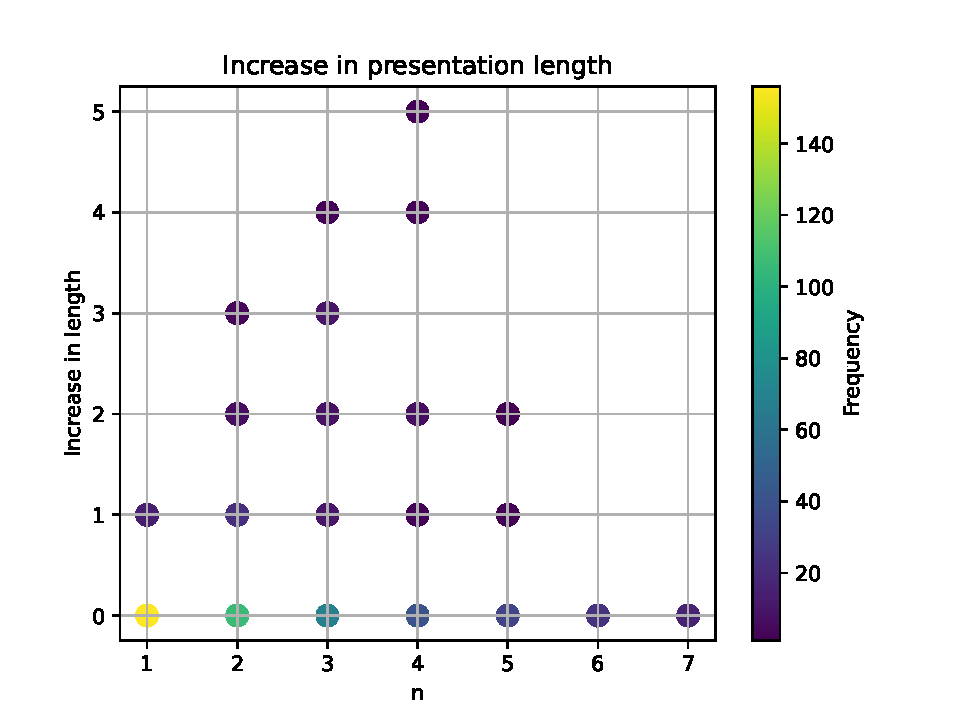
\includegraphics[width=1.1\textwidth]{fig/gs_length_increase_vs_n.pdf}
		\caption{Distribution versus $n$.}
		\label{fig:gs_length_increase_vs_n}
	\end{subfigure}
	\caption{The maximum increase in the length of a presentation relative to its initial length along the AC trivialization path. The increase is plotted as a function of the initial length of the presentation on the left and as a function of $n$ on the right.} \label{fig:gs_length_increase}
\end{figure}

\begin{figure}
	\centering
	\begin{subfigure}[b]{0.4\textwidth}
		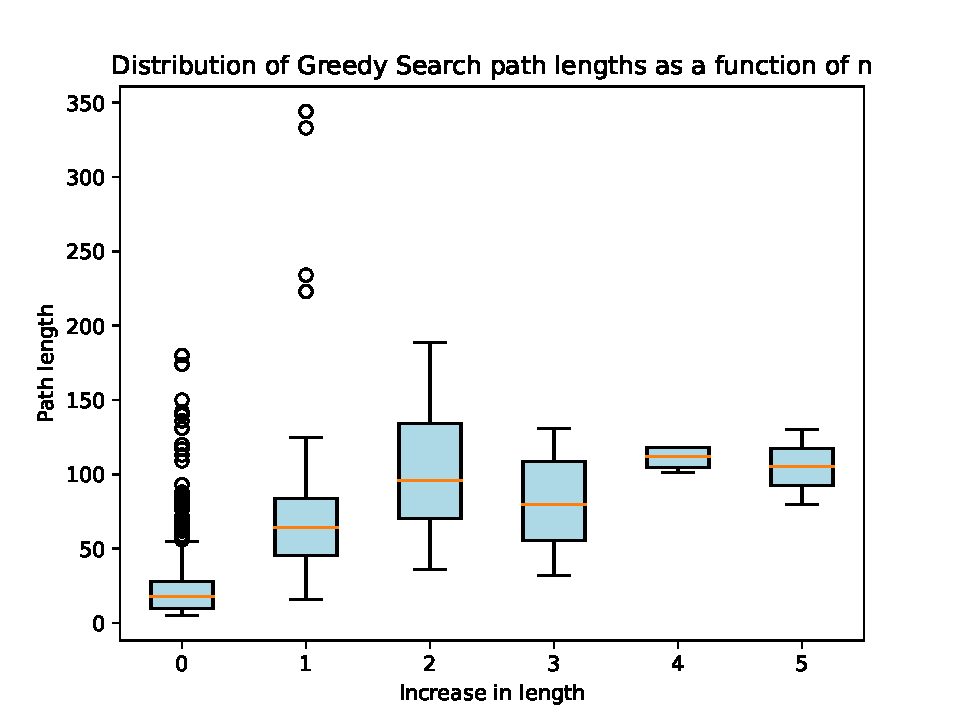
\includegraphics[width=\textwidth]{fig/path_lengths_vs_length_increase.pdf}
		\caption{Distribution versus maximum increase in presentation length.}
		\label{fig:path_lengths_vs_length_increase}
	\end{subfigure}
	\begin{subfigure}[b]{0.4\textwidth}
		\centering
		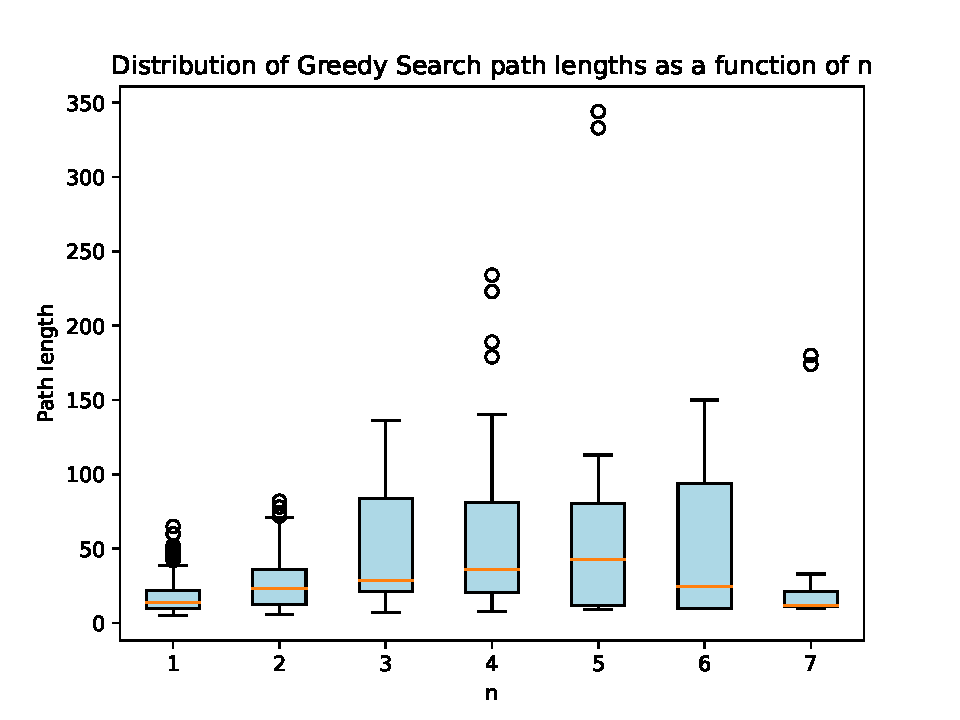
\includegraphics[width=1.1\textwidth]{fig/gs_path_lengths.pdf}
		\caption{Distribution versus $n$.}
		\label{fig:gs_path_lengths}
	\end{subfigure}%
	\caption{Distribution of lengths of AC-trivialization paths learned by greedy search as a function of maximum increase in presentation length (left) and $n$ (right).} \label{fig:gs_path_length}
\end{figure}

\subsection{AC-triviality of $\MS(1, w)$} \label{sec:ms1w_}

As mentioned in the previous subsection, the greedy search could solve all $n=1$ presentations of the Miller--Schupp series in our dataset. This motivated us to prove AC-triviality for all $\MS(1, w)$. 

In this and the following subsections, we frequently use the \emph{substitution} transformation mentioned in Section~\ref{sec:AC}.   

% The proof of this result, along with the results we present in the next section, relies on the substitution principle: \todo{Shehper: I am confused about how to present the substitution principle. 1. Should we skip Burns-Macedonska result and just mention the principle as we use it? This is exhibited in the example that follows. 2. Should we mention the substitution principle in Section 2 instead of here, right after we describe AC moves? 3. In section 8, we describe a substitution principle of stable AC conjecture. The first line of that proof is essentially what we need in this section. Should we refer our vanilla AC substitution lemma in the proof of that lemma?}

% \begin{lemma}[Burns, Macedonska, \cite{BurnsI}]\label{l:BM}
%     Let $P = \angles{x_1, \cdots, x_n \mid r_1, \cdots, r_n}$ be a presentation of the trivial group. $P$ is AC-equivalent to the presentation $\angles{x_1, \cdots, x_n \mid r_1, \cdots, r_{i-1}, r'_i, r_{i+1}, \cdots, r_n}$ where $r'_i$ is congruent to $r_i$ modulo the normal closure of  $\{r_1, \cdots, r_{i-1}, r_{i+1}, \cdots, r_n\}$.
% \end{lemma}

% \lucas{if I understand correctly, the lemma is also a consequence of the example that follows. I think it might be better for non-mathematical readers to present it in that language, espeically given that's how we use it. And then @Shehper I agree we should cite it in the stable section. But my overall preference would be to not state this as a lemma and just mention it when we use it} A simple consequence of this lemma is that we may substitute one relation into others. As an example, consider the presentation $\angles{x, y \mid xy = y^2 x, u x y v = e}$ where $u$ and $v$ are some words in $x$ and $y$. We will show that it is AC-equivalent to the presentation $\angles{x, y \mid xy = y^2 x, u y^2 x v}$ obtained by substituting the first relator into the second. First, use conjugation by $v$ to write the second relator as $vuxy$. Next, write the first relator as $(xy)^{-1} y^2 x$, and multiply the second relator by it. We get $vuy^2 x$, which we may conjugate by $v^{-1}$ to get the required result. 

\begin{theorem}\label{t:ms1wt}
    $\MS(1,w)$ is AC-trivial for all $w$.
\end{theorem}

\begin{proof}
We have 
\[
\MS(1, w) = \angles{x, y \mid x^{-1} y x = y^{2}, x = w}
\]
where $w$ has exponent sum 0 in $x$. We can re-write the first relator in the following four ways: 
\begin{enumerate}[label=(\roman*)]
    \item $yx=xy^2$
    \item $x^{-1}y = y^2 x^{-1}$
    \item $x^{-1}y^{-1}=y^{-2}x^{-1}$
    \item $y^{-1}x = xy^{-2}$
\end{enumerate}

We can substitute these equations in the second relator to move around all occurrences of $x$ and $x^{-1}$: relations (i) and (iv) move $x$ to the left, relations (ii) and (iii) move $x^{-1}$ to the right. We continue until the second relator becomes $x^{a-1} y^b x^{-a}$ for some $a, b \in \mathbb{Z}$. Through conjugation, this simplifies to $x = y^b$, which when substituted into the first relator leads to a trivialization of the presentation.
\end{proof}

The following result follows from this theorem.

\begin{theorem}\label{t:msnw}
    $\MS(n, w_\star)$ for $w_\star = y^{-1} x y x^{-1}$ is AC-trivial for all $n$.
\end{theorem}

\begin{proof}
In the presentation,
\[
\MS(n, w_\star) = \angles{x, y \mid x^{-1} y^n x = y^{n+1}, x = y^{-1} x y x^{-1} }
\]
we can rewrite the second relation as $y^{-1} x y = x^2$, and apply the automorphism $x \leftrightarrow y$ to get
\[
\MS(n, w_\star) = \angles{x, y \mid
x^{-1} y x = y^2 , y^{-1} x^n y = x^{n+1}}.
\]
This presentation is the same as $\MS(1, y^{-1} x^n y x^{-n})$, which is AC-trivial by \cref{t:ms1wt}. 
\end{proof}

AC-trivializations of $\MS(n, w_\star)$ for $n = 3, 4, 5, 6, 7, 8$ were recently obtained using automated theorem proving in \cite{new-ac-for-ms}. Here, we have obtained AC-trivializations of this family for all $n$.


% Indeed, to see how to realize this with AC moves, consider by means of example the application of (1) to $w_1yxw_2$. First, we cycle the relator to get $yxw_2w_1$, then invert it to get $w_1^{-1}w_2^{-1}x^{-1}y^{-1}$, and then multiply by (1) written as $yxy^{-2}x^{-1}$ onto the end of the relator, giving $w_1^{-1}w_2^{-2}y^{-2}x^{-1}$. Inverting again and cycling gives us $w_1xy^2w_2$. 

% After moving all positive powers of $x$ to the left and negative powers of $x$ to the right, we can cancel them with (AC3) by conjugating by $x^{-1}$. We are then left with $y^kx^{-1}$ for some $k$, since the exponent sum on $x$ in the second relator was $-1$ to begin with and is unchanged throughout these moves. Substituting this into the first relation, we get $y=y^2$ or $y=1$, from which we can easily trivialize the second relator as well. 


\subsection{Length reduction for $\AK(n)$}
\label{sec:len-reduction}

In \cref{sec:search-ms}, we discussed the performance of classical search algorithms for presentations of the Miller--Schupp series. But what if we apply these algorithms for presentations of the Akbulut--Kirby series instead? We find that starting from $AK(5)$---a presentation of length $17$---and performing greedy search for $20$ million nodes, reduces its length to 16. Examining the sequence of AC moves connecting the two presentations, we found the following result.\shehper{@Anibal, all: Two paper-wide issues to mention here: 1. Should we try to match numbering of theorems in introduction with their numbering in later sections, and 2. when we cref lemma or proposition, it is referenced as a Theorem instead. I dont know how to fix that..}

\begin{theorem}\label{t:n+11}
	For every $n\geq 2$, $\AK(n)$ is AC-equivalent to the presentation
	\[
	\angles{ x,y \mid x^{-1} y x = x y x^{-1} y \ ,\  xyx=yx^{n-1}y },
	\]
	of length $n+11$. This gives reduction in length of $AK(n)$ for all $n \geq 5$.
\end{theorem}

To prove this theorem, we will  use the following result due to \cite{MMS}, and prove two additional theorems (\cref{t:mswk_wk1} and \cref{t:ms-short}). From these results, \cref{t:n+11} follows immediately. 

\begin{proposition}
    [Myasnikov, Myasnikov, and Shpilrain, \cite{MMS}]\label{t:MS-AK-MS}
    For all $n \geq 2$, $AK(n)$ is AC-equivalent to $\MS(n, w_1)$ where $w_1 = y^{-1} x^{-1} y x y$.
\end{proposition}

\begin{theorem}\label{t:mswk_wk1}
    For each fixed $n > 0$, the 1-parameter family of presentations $\MS(n, w_k)$ are all AC-equivalent. Here, $w_k = y^{-k} x^{-1} y x y$ is parameterized by $k \in \mathbb{Z}$. 
    % \shehper{@Lucas (requires work): I wonder if we can find a similar result for $MS(n, w'_l)$ where $w'_l = y^{-1} x^{-1} y^l x y$. That is, all elements of this family are AC-equivalent. This would lead to AC-triviality of $AK(3)$ (and possibly $AK(n)$) as the case $l=-3$ is known to be AC-trivial: it is presentation 403 in our greedy solved presentations.txt file on GitHub. Similarly, a result for $y^{-1} x^{-1} y x y^p$ might also be useful. }
\end{theorem}


\begin{proof}
    Starting with the presentation,
        \[
\MS(n, w_k) = \angles{x, y \mid x^{-1} y^n x = y^{n+1}, x = y^{-k} x^{-1} y x y},
\]
    we will show that for any fixed $n$ and $k$, $\MS(n, w_k)$ is AC-equivalent to $\MS(n, w_{k+1})$.

    First, note that the first relation in $\MS(n, w_k)$ can be rearranged in the following three ways:
    \begin{enumerate}[label=(\roman*)]
        \item Multiplying by $y^{k-n}x$ from the left and by $y^{-1}$ from the right gives 
        \[
            y^kxy^{-1}=y^{k-n}xy^n.
        \]
        \item Multiplying by $y^{-1}$ from the left and by $x^{-1}y^{-1}$ from the right, and inverting the relation gives 
        \[
            y^{-(n-1)}xy = yxy^{-n}.
        \]
        \item Multiplying by $y^{-1}x$ from the left and by $y^{k-n}$ from the right, and inverting the relation gives
        \[
            y^{n-k}x^{-1}y^{-(n-1)}=y^{-(k+1)}x^{-1}y.
        \]
    \end{enumerate}

    Now, we can rearrange the second relation  to get $y^k x y^{-1}=x^{-1}yx$. Substituting (i) gives $y^{k-n} x y^n = x^{-1}yx$, which  we can rewrite as $yxy^{-n}=xy^{k-n}x$. Now substituting (ii) gives $ y^{-(n-1)}xy= xy^{k-n}x$, which we may rewrite as $y^{n-k}x^{-1}y^{-(n-1)}=xy^{-1}x^{-1}$. Finally, substituting (iii) gives $y^{-(k+1)}x^{-1}y=xy^{-1}x^{-1}$, which is equivalent to $x=y^{-(k+1)}x^{-1}yxy=w_{k+1}$. 
\end{proof}

\begin{theorem}\label{t:ms-short}
    For each $n > 0$ and $k \in \mathbb{Z}$, $\MS(n, w_k)$ is AC-equivalent to the presentation
    \[P(n, k) = \angles{x, y \mid  y^{n-k-1}  x^{-1} y x = x y x^{-1} y^{n-k} \ , \ x = y^{-k} x^{-1} y x y },
    \]
    of total length $|k| + |n - k| + |n - k - 1| + 11$. For each fixed $n$, this length is minimum when $k=n-1$, which gives the presentation
    \[P(n, n-1) = \angles{x, y \mid   x^{-1} y x = x y x^{-1} y \ , \ x = y^{-(n-1)} x^{-1} y x y },
    \]
    of length $n+11$.
\end{theorem}

\begin{proof}
    Starting with the presentation,
        \[
        \MS(n, w_k) = \angles{x, y \mid x^{-1} y^n x = y^{n+1}, x = y^{-k} x^{-1} y x y},
        \]
    the second relation may be equivalently expressed as 
    \begin{enumerate}[label=(\roman*)]
        \item $y^{k}xy^{-1}=x^{-1}yx$
        \item $y^{-1}xy^{k}=xyx^{-1}$
    \end{enumerate}
    Multiplying the first relation by $y^{-1} x$ from the left and by $y^{-1}$ from the right, we get $y^{n-1} x y^{-1} = y^{-1} x y^{n}$, which we may rewrite as $y^{n-k-1} \left(y^k x y^{-1}\right) = \left(y^{-1} x y^{k}\right) y^{n-k}$. Substituting from (i) on the LHS and from (ii) on the RHS gives the required result.
\end{proof}

Combining the previous three results shows that, for each fixed $n$, $AK(n)$ is AC-equivalent to all members of the infinite families $\MS(n, w_k)$ and $P(n, k)$. From this, \cref{t:n+11} follows immediately from setting $k = n - 1$.

\begin{remark}
While $P(n, n-1)$ is always the shortest presentation from the $P$ family, other $P(n, k)$ may also give reductions in length of $\AK(n)$. To find which presentations of $P$-family are shorter than $\AK(n)$, we compare the length of $\AK(n)$, i.e. $2n + 7$, with the length of $P(n, k)$ given by:
\[
    \begin{cases} 
        2n + 10 - k, & \text{if } k \leq n-1, \\
        3k + 12 - 2n, & \text{if } k \geq n.
    \end{cases}
\]
This is less than $2n+7$ when $4 \leq k \leq n-1$ or $n \leq k < \frac{1}{3} \left(4n-5 \right)$.
\end{remark}

We also note that the AC-triviality of $\AK(2)$, when combined with \cref{t:mswk_wk1}, gives the following result. 
\begin{corollary}\label{c:ms2wk}
Each member of the infinite families $\MS(2, w_k)$ and $P(2, k)$ is AC-trivial.
\end{corollary}



\subsection{Limitations and extensions}

While the greedy search algorithm performs better than the breadth-first search, it has some of the same limitations.
Namely, it is memory inefficient, and we cannot leverage the parallelizability of modern hardware architectures.
It also does not learn a general algorithm that would find an AC trivialization for any given balanced presentation.

Reinforcement learning algorithms, particularly policy gradient algorithms, present a promising alternative that avoids these downsides.
These algorithms are memory efficient and can be trained in a highly distributed manner, which we will focus on in the next section.

Another interesting direction to pursue involves changing the sorting function used by greedy search. Consider the family of greedy search algorithms where the priority queue is sorted by a fixed function $f: (r_1, r_2) \to \mathbb{R}$ which takes a presentation and outputs a real number\footnote{We can also reinterpret breadth-first search in this manner if, given as input to $f$ the path length $l$, we have the function return $l$. From this perspective it becomes clear that, whenever breadth-first search succeeds, it finds a path of minimal length.}. The greedy search algorithm used here is based on the function $f(r_1, r_2) \to |r_1| + |r_2|$. An interesting option would be to use machine learning to try and learn a good function $f$. This idea is inspired by search-based reinforcement learning systems, such as AlphaGo and AlphaZero, which combine Monte Carlo Tree Search with learned heuristics to evaluate and prioritize states dynamically. While these systems go beyond classical greedy search by incorporating exploration and planning through tree-based rollouts, the core principle of leveraging a learned heuristic function to guide search is analogous.
	% !TEX root = ../ac_paper.tex

\section{Reinforcement Learning}

\subsection{Markov Decision Process}

We will model the problem underlying the Andrews-Curtis conjecture as a Markov Decision Process (MDP).
An MDP is a tuple of data $(S, A, P, R, \rho)$ where
\begin{itemize}
	\item $S$ is a set of states called the state space.
	\item $A$ is a set of actions that acts on $S$, called the action space.
	That is, each element $a \in A$ is a map $a \colon S \to S$.
	\item $P \colon S \times A \times S \to \mathbb{R}$ is the transition
	probability function.
	It is the probability $p (s' | a, s)$ of reaching
	state $s'$ as we take action $a$ in state $s$.
	\item $R \colon S \times A \times S \to \mathbb{R}$ is the 'reward' function.
	\item $\rho$ is the initial probability distribution of states.
\end{itemize}

In the setting of the Andrews-Curtis conjecture, $S$ is the set of all presentations of the trivial group, and $A$ is the set of AC moves.
The transition probability function $P$ is the probability of applying a particular AC move to a given presentation.
The choice of reward function $R$ is up to us.
One suitable option (the only one we have worked with so far) is to take $R(s)$ for a presentation $s$ to be the negative of the total word length ---i.e., the sum of word lengths of each relator in the presentation.
(AK(3) has a total word length of 13.)
This choice depends only on the final state $s'$ and is independent of the initial state $s$
or the action $a$.
\footnote{Another good choice could be the difference in total word lengths of the final and the initial states.} It is suitable for the goal of trivializing a presentation as the trivial presentation has the maximum possible reward value: negative of the number of generators.

Differences in our AC moves and the usual notion of AC moves: 1.
since we restrict lengths, our AC moves are not invertible; 2.
we use full-simplify which cyclically reduces words before returning the answer.
For example, if we conjugate a word and it takes the form $y \cdots y^{-1}$, our conjugation operation returns $\cdots$.

\fixme{Things to try: change the initial state distribution to include canonic representations of certain lengths.}

\fixme{If we have a "good" policy for a small max length $k$, a new "good" policy for a larger max length $k'$ should do one of two things things: i).
for state $s$ with length $< k$ and with $a(s) $ also of length $< k$ for all $a$, $\pi(s)$ should be the same; ii) learn new optimal policy i.e. new $\pi(s)$ for all other $s$ starting with random policy.
This kind of states include states of length $> k$ as well as states of length $< k$ for which $a(s) $ has length $> k$ for some $a$.}

\fixme{When we increase max length, value of states of type i) could still change.
We could replace the condition in i) by the condition that states $s$ are trivializable.
but even then, their values could change.
In particular, an optimal policy function might become sub-optimal (restricted to states of smaller length) when max length is increased.}

\subsection{Proximal Policy Optimization}

https://arxiv.org/pdf/2110.00641.pdf

\fixme{Maybe change the terminal state in RL to be the one where either relator is of length 1 --- as that essentially implies triviality of the presentation.
Does that also mean the reward should be -min(lengths)?}

\subsection{Results}

\begin{enumerate}
\item Shorter sequences of AC moves. 
\end{enumerate}

\subsection{Future directions}
Scaling?
	\section{The Cure: New Algorithms}\label{sec:algo}

In previous sections we explained from a variety of different perspectives that the Andrews-Curtis conjecture is a good example of a mathematical problem where the length of a solution can be much greater than the length of the initial presentation, in some cases with purely analytical lower bounds that are hyperexponential in the size of the input. In particular, we saw that small increases in presentation length under 20 quickly lead to solution lengths in the range of hundreds and higher, quickly exceeding the number of moves in the longest game of chess.

If solving a mathematical problem required finding a path of length $L$, say with $L=10^6$, an RL agent would be pretty much out of luck under circumstances of a typical hard search problem, where the number of successful paths is exponentially suppressed by $L$. The good news is that in mathematics --- and in many other domains --- such hard search problems never come in isolation. Rather, there is a distribution of problems such that generic instances are ``easy'' and a small fraction is ``hard.'' Learning this distribution for smaller values of $L$ contains the crucial information for solving new cases at the next increment of $L$.

\subsection{Supermoves}

In automated reasoning or search problems where the minimal length solution has a theoretical lower bound that by far exceeds computational capabilities, it is clear that direct approach with fixed size steps is not going to succeed, unless the problem is easy and a large fraction of long paths meets the desired criteria. In order to reach extraordinary path lengths, one must allow progressively longer sequences of elementary moves to be added to the action space. Although this general strategy seems unavoidable in problems like the AC conjecture, it leads to many practical questions. For example, what should be the selection criteria for such ``supermoves''? And, how often should they be added to the action space?

In the context of the AC conjecture, a good example of such supermoves are the ``elementary M-transformations'' \cite{BurnsI, BurnsII}. These transformations trivialize $\AK(2)$ in just two steps, even though this presentation is known to admit the shortest AC trivialization path of length 14. A downside of elementary M-transformations, though, is that they are infinite in number, which complicates their application in classical search techniques.

In our study, we explored the idea of identifying AC supermoves by selecting some frequently occurring subsequences of AC moves in the paths discovered by Proximal Policy Optimization (PPO). By extending the action space $A$ of the Markov Decision Process (MDP) with these subsequences and checking whether this enhanced action space helps our agent discover shorter paths of trivialization, we learned a few useful lessons:

\begin{itemize}

\item First, it helps to augment the action space with subsequences of different kind that include frequently occurring compositions of elementary moves as well as very rare ones.

\item  Also, in the early stage it helps to introduce several supermoves at once.

\item And, at later stages it helps to allow removing actions from the action space, not only adding them.
    
\end{itemize}

\noindent
Not following these empirical rules, e.g. introducing too few supermoves initially or too many over the entire length of the training process, leads to considerable reduction in performance of the RL agent. Even in the most optimal regimes that we were able to find, the improvement of the performance due to supermoves was rather modest, leading us to explore other alternatives.

\begin{figure}
	\centering
	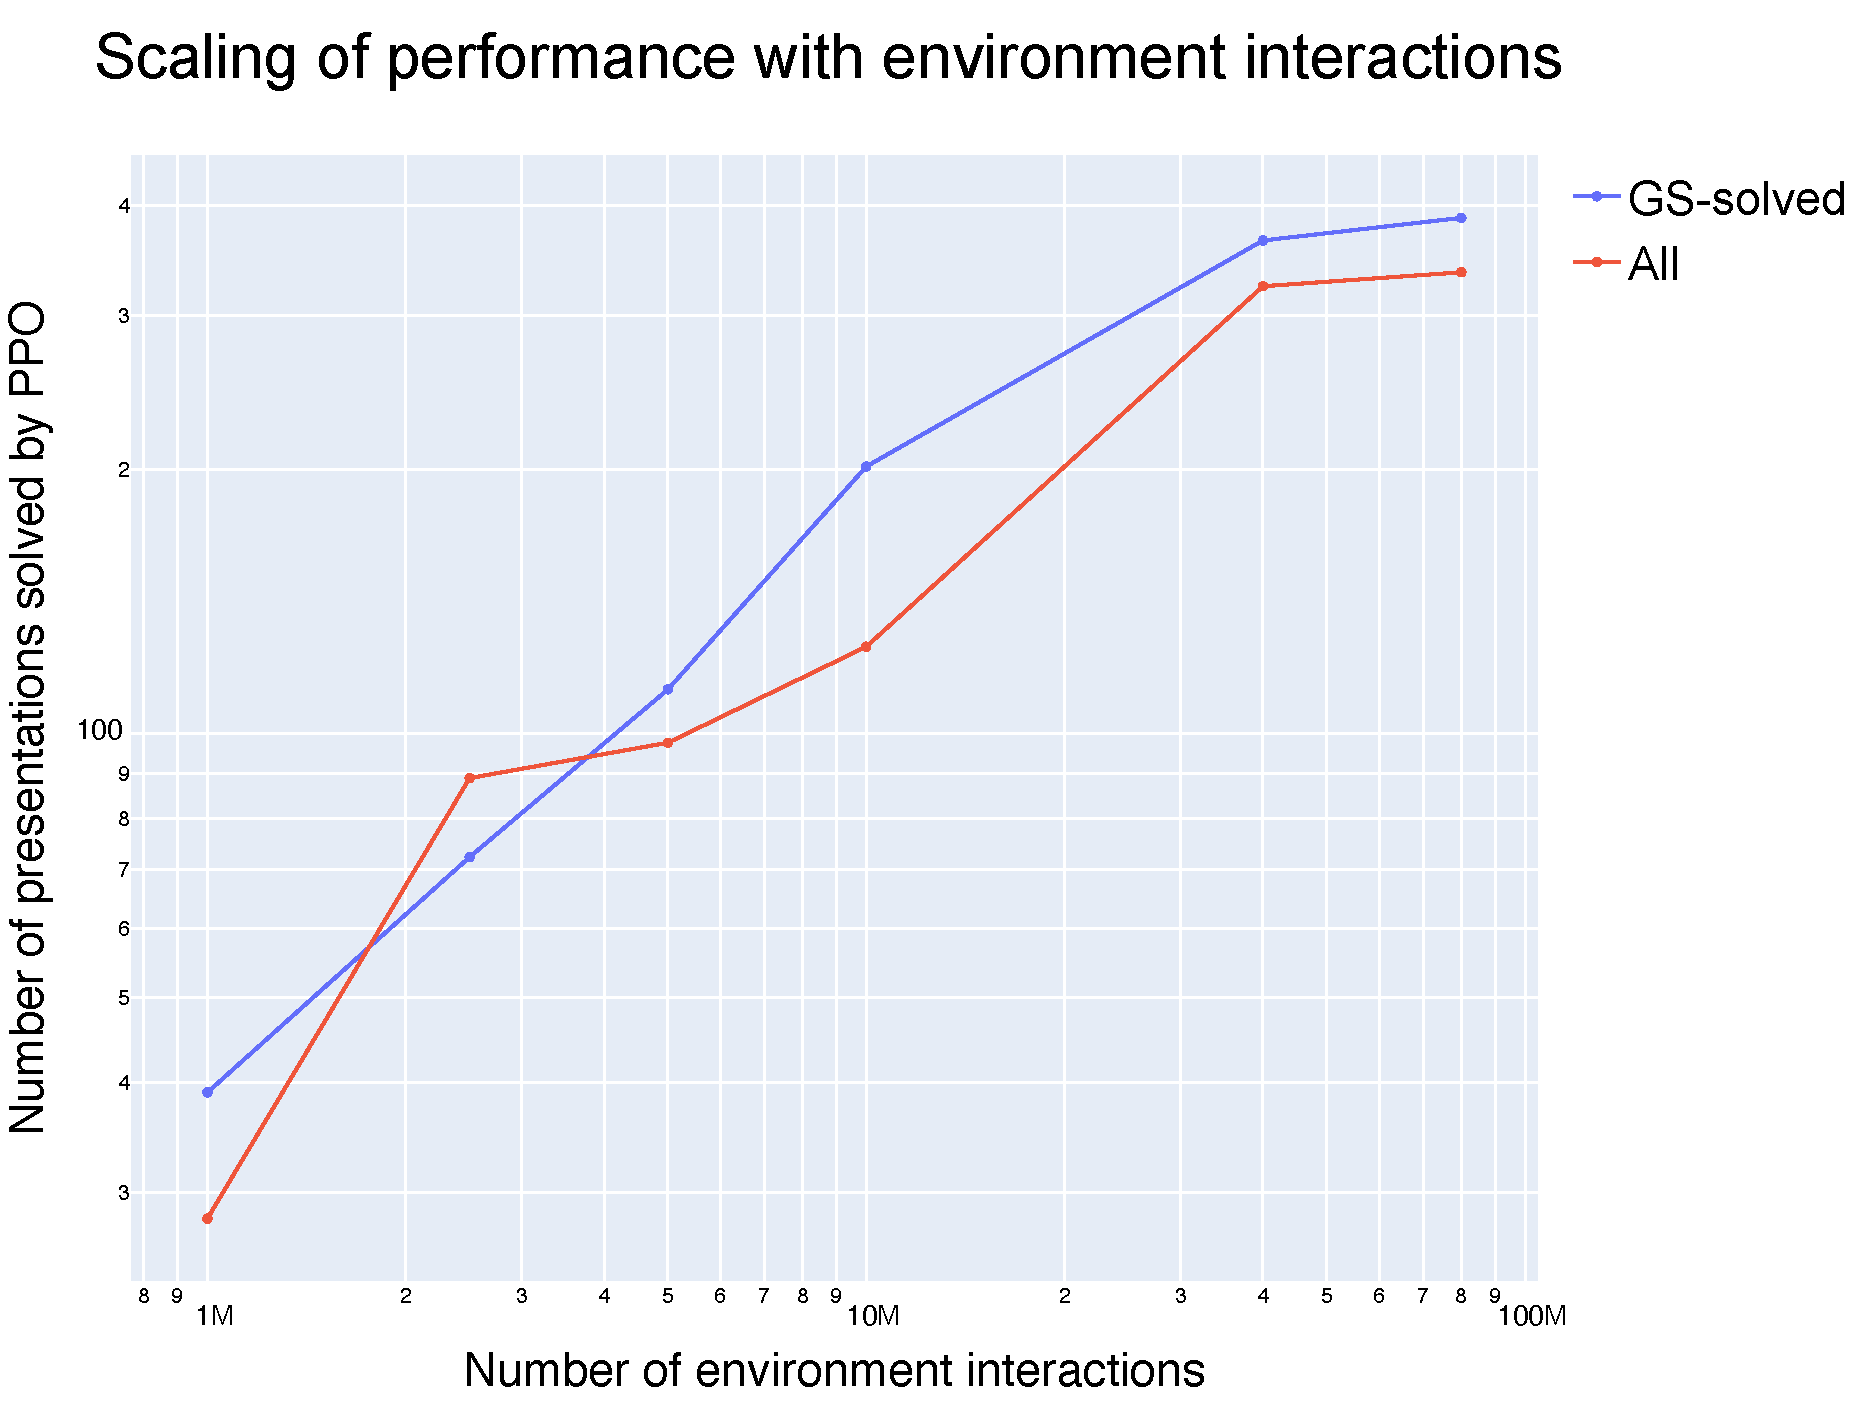
\includegraphics[scale=0.35]{fig/scaling_env.pdf}
	\caption{Number of AC presentations solved by our PPO agent as a function of the number of training steps. Here, \textit{GS-solved} refers to a subset of the Miller-Schupp dataset of \autoref{sec:search} that was solved by the greedy search algorithm.}
	\label{fig:scaling_env}
\end{figure}

\subsection{The anatomy of success}
%\subsection{New self-improving algorithms}

While supermoves clearly need to be a part of the solution in hard problems like the AC conjecture, much of the success depends on the criteria for selecting them. Here, we advocate for a dynamic approach where the network itself learns the criteria for selecting supermoves, in addition to the best ways to implement them. One realization of this approach could be a multi-agent model, where one network is learning to play the game and the other is learning the rules for changing the action space (adding and removing supermoves). We hope that future iterations of this strategy can lead to AI systems that can `learn how to learn' dynamically by making both algorithmic and architectural changes through collecting the information about hard instances.\footnote{Here, by self-improving AI systems we mean algorithms that have the ability to ``interpolate'' between off-the-shelf algorithms such as A2C and TRPO, as well as a myriad of custom algorithms that do not even have a name. Clearly, this level of technology is not presently available, and one of the key points of this section is that developing such systems should be based on the hardest instances the agent encounters.}

\begin{figure}
	\centering
	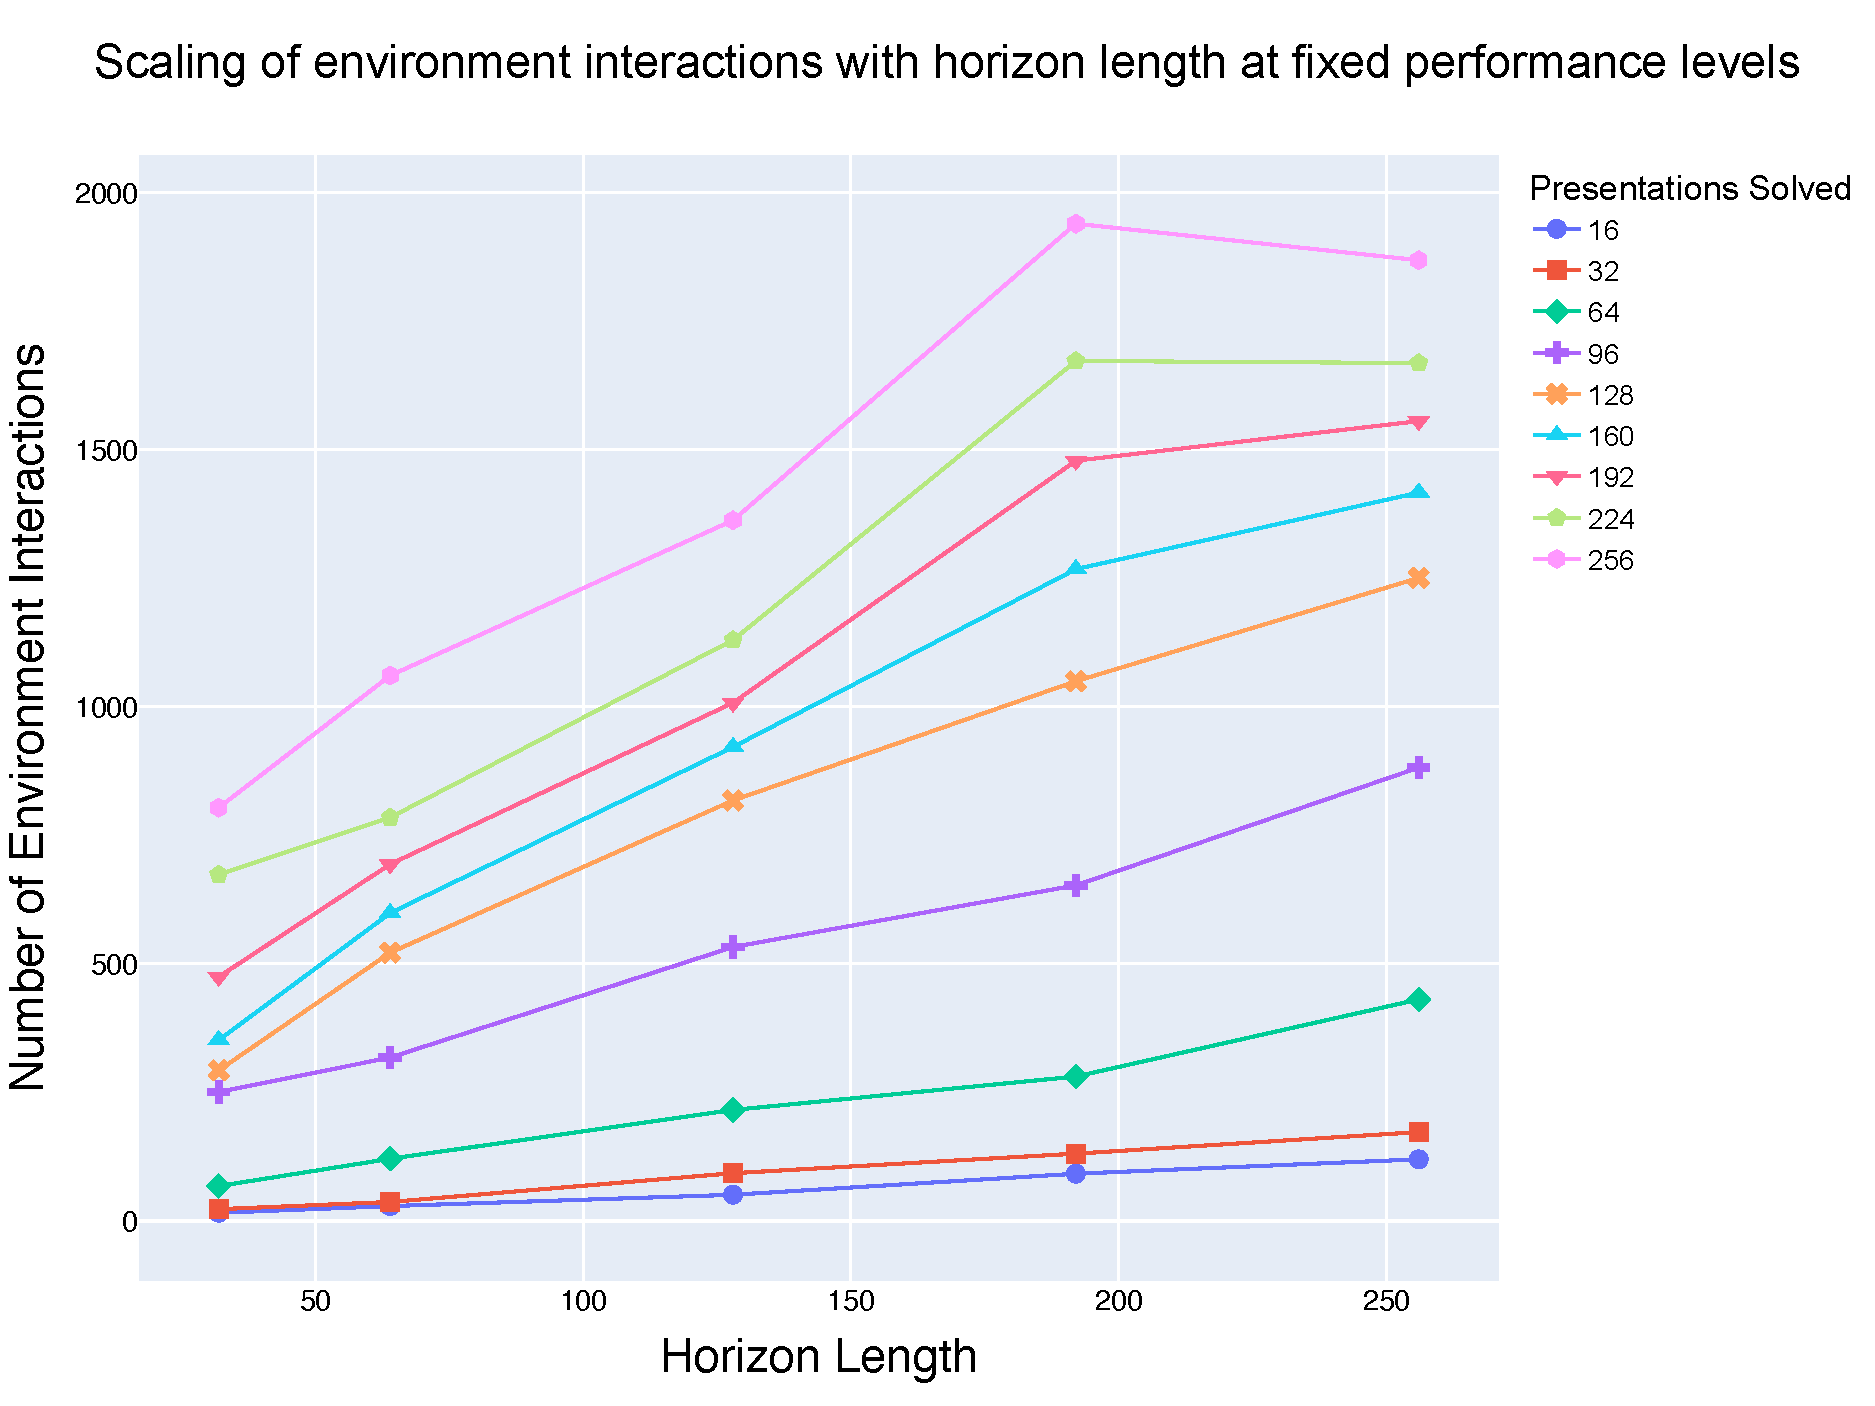
\includegraphics[scale=0.35]{fig/env_vs_horizon.pdf}
	\caption{To maintain consistent performance, increasing the horizon length requires a roughly linear increase in the number of training steps (environment interactions).}
	\label{fig:env_vs_horizon}
\end{figure}

Specifically, suppose $N$ is one of the characteristics of either the algorithm or the architecture that has non-trivial impact on performance. In practice, there can be several such parameters, but for simplicity we explain the idea as if there is only one.\footnote{Analyzing a multi-dimensional landscape is generally a good idea, as it can yield better performance improvements, but the price to pay is that changes of different characteristics become correlated, as illustrated in \autoref{fig:env_vs_horizon}.} Then, from the practical standpoint, a natural notion of hardness is such that \textit{hard instances} are defined to be those which the model can solve at the current setting of $N$ and not with the lower value of the resource $N$. In addition, in search problems we include the length of the path in the notion of hardness, i.e. select a subset of the instances that the model could solve through especially long paths. Note, by the very nature of the search problem we are interested in, there can not be too many such hard instances at each step of increasing $N$, for otherwise the problem would be easy, not hard. Collecting the information about the hardest instances at each increment in $N$ can be used to select supermoves, e.g. as subsequences of the sequences of moves that solve the hard instances. \autoref{alg:adaptive_ai_model} provides one particular realization of this idea.

\begin{algorithm}
	\caption{Adaptive AI Model Training and Path Discovery}
	\label{alg:adaptive_ai_model}
	\begin{algorithmic}[1]
		\State \textbf{Input:}
		\begin{itemize}
			\item[] Family of AI models $\pi(N)$ with common state space $S$ and action space $A_0$
			\item[] Initial setting $N_0$ and ordered range $\{N_1, N_2, \ldots, N_{\text{max}}\}$
			\item[] Number of epochs for training
			\item[] Validation set $V \subset S$
			\item[] Distinguished state $s_0 \in S$
			\item[] Positive integer $n$
		\end{itemize}
		
		\State \textbf{Output:}
		\begin{itemize}
			\item[] For each setting $N_i$: Set of pairs $\{v, P\}$ where $v \in V$ and $P$ connects $v$ to $s_0$
		\end{itemize}
		
		\State Initialize $A(N_1) \gets A_0$
		
		\For{each $N_i$ in $\{N_1, N_2, \ldots, N_{\text{max}}\}$}
		\State Train model $\pi(N_i)$ on $S$ for the given number of epochs
		\State Evaluate $\pi(N_i)$ on $V$ to discover paths connecting $V$ to $s_0$ using $A(N_i)$
		
		\State $V(N_i) \gets \{ v \in V \mid v$ can be connected to $s_0$ using $A(N_i)$, but not by any $\pi(N_j)$ with $j < i\}$
		\State $W(N_i) \gets \{ v \in V(N_i) \mid$ the longest path connecting $v$ to $s_0$ using $A_0 \}$
		
		\If{$i \geq n$}
		\State Compare $W(N_{i-n+1})$ to $W(N_i)$
		\State Adjust $A(N_{i+1})$ based on the comparison
		\Else
		\State $A(N_{i+1}) \gets A(N_i)$
		\EndIf
		\EndFor
	\end{algorithmic}
\end{algorithm}

In the context of the AC conjecture, examples of the metric $N$ can be the horizon length or the number of interactions with the environment. As \autoref{fig:scaling_env} illustrates, increasing the number of environment interactions leads to a larger number of non-trivial presentations from the Miller-Schupp series being solved (i.e. AC-trivialized) by our RL agent. Moreover, the length of the AC trivialization path also grows for some of the solutions (but not all).
%
Therefore, in order to implement the program outlined above in the specific context of the AC conjecture, we can focus on the longest AC trivialization paths that the model is able to find at each value of $N$.

\begin{figure}[h]
    \centering
    \begin{subfigure}{0.45\textwidth}
        \centering
        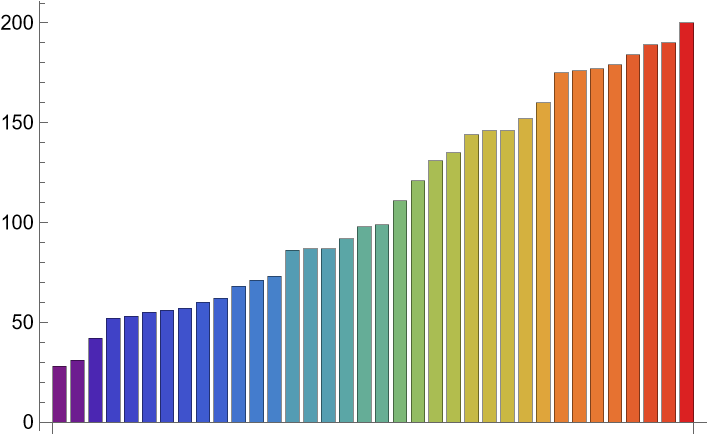
\includegraphics[width=\textwidth]{fig/all_path_length_80M.png}
        \caption{all}
        \label{fig:all_path_length_80M}
    \end{subfigure}
    \hfill
    \begin{subfigure}{0.45\textwidth}
        \centering
        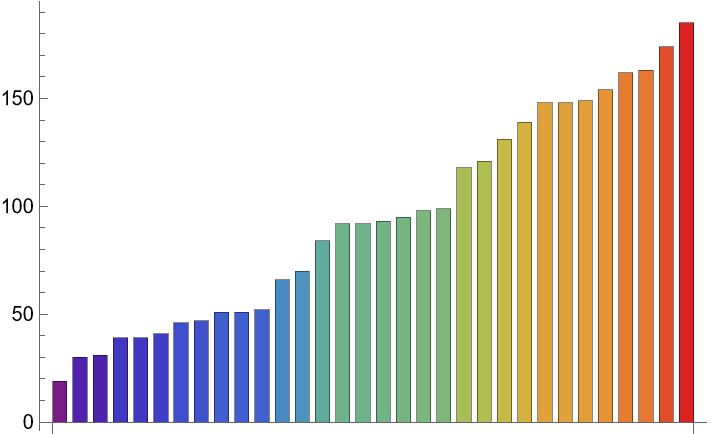
\includegraphics[width=\textwidth]{fig/solved_path_length_80M.png}
        \caption{GS-solved}
        \label{fig:solved_path_length_80M}
    \end{subfigure}
    \caption{Path length distributions for AC presentations solved by the RL agent at $N=8 \times 10^7$ from \textit{all} and \textit{GS-solved} datasets are nearly identical. In both cases, hard instances are shown in red.}
    \label{fig:path_length_80M}
\end{figure}

Collecting this information in the process of training can be used to introduce (and remove) supermoves to the action space in a dynamic fashion. There can be many different implementations of this idea that we plan to explore more fully elsewhere. For example, one can consider selecting all or subset of the longest AC trivialization paths that the model finds at each $N$. Out of those, in each case, one can consider selecting the entire trivialization path or a subset, randomly or non-randomly. Alternatively, one can compare the longest trivialization paths at several (consecutive) values of $N$ and choose subsequences of moves that are shared by several long trivializaion paths at different $N$.

For example, if $N$ denotes the number of interactions with the environment, we did a few preliminary experiments with the dataset of \autoref{sec:rl} and several different seed values. To illustrate the effects of stochastisity, let us consider $N=8 \times 10^7$. The agents with five different seed values were able to solve 354, 337, 330, 328, and 323 presentations, respectively. And their average, $334.4$, is shown in \autoref{fig:scaling_env}. Many of these AC presentations can be solved at the earlier stage, with $N=4 \times 10^7$ or less. If in the definition of \textit{hard instances} we require that they are solved by \textit{all} five agents, there are only 5 presentations total. On the other hand, if we require that they are solved by \textit{any} of the 5 agents, the number goes up to 36.

\begin{figure}[h]
    \centering
	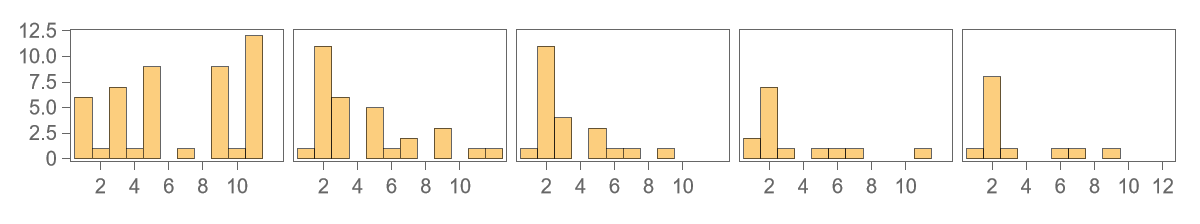
\includegraphics[scale=0.6]{fig/anatomy_all.png}
	\caption{Types of AC moves that appear in trivialization paths of 5 presentations solved by all 5 agents at $N=8 \times 10^7$. The move $\# 2$ occurs disproportionately more frequently. There are 12 different types of basic AC moves described in \autoref{sec:search}.}
	\label{fig:anatomy_all}
\end{figure}

Moreover, not surprisingly, the 5 presentations solved by all 5 agents have considerably shorter path lengths --- 47, 31, 22, 14, and 13 --- compared to path lengths of the 36 presentations illustrated on the left panel of \autoref{fig:path_length_80M} that go up to $200$. Both 5 presentations solved by all agents and 36 presentations solved by at least one of the agents provide viable options for defining hard instances and, in turn, selecting supermoves. However, they lead to qualitatively different results. For example, all 5 presentations solved by all 5 agents are solved at a smaller value of $N$ when required to be solved by only one of the agents. More importantly, they have very different anatomy, illustrated in \autoref{fig:anatomy_all} and in \autoref{fig:anatomy_some}, respectively.
%
By examining the longest trivialization paths of the 36 presentations solved by at least one agent at $N=8 \times 10^7$, we often see long strings of moves $\# 5$ and $\# 11$, interlaced with moves $\# 3$, $\# 7$, and $\# 9$. These are our top candidates for the supermoves to be added at $N=8 \times 10^7$.
%
Note that moves $\# 4$ and $\# 8$ are least common in the examples presented in both \autoref{fig:anatomy_all} and \autoref{fig:anatomy_some}.

\begin{figure}[h]
    \centering
	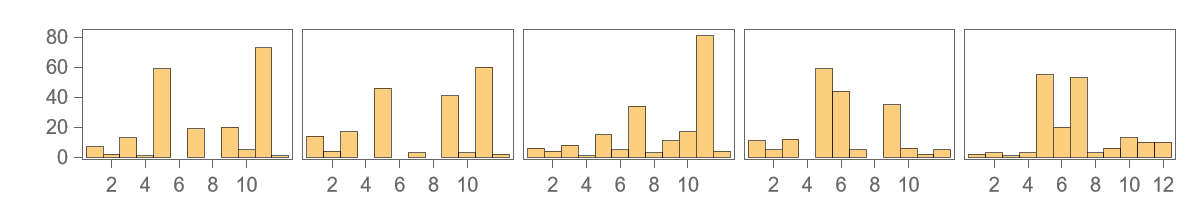
\includegraphics[scale=0.6]{fig/anatomy_some.png}
	\caption{Types of AC moves in the 5 longest trivialization paths --- of length 200, 190, 189, 184, and 179 --- found by at least one agent at $N=8 \times 10^7$. The most frequent moves are $\# 5$, $\# 7$, $\# 9$, and $\# 11$. There are 12 different types of basic AC moves described in \autoref{sec:search}.}
	\label{fig:anatomy_some}
\end{figure}

As in other parts of this paper, we performed the analysis on two datasets of sizes 1190 and 533 that, respectively, contain all members of the Miller–Schupp family with $n \leq 7 \, \land \, \length(w) \leq 7$ and only those solved by the greedy search. The results are qualitatively similar, as we already saw in \autoref{fig:path_length_80M} that illustrates length distributions of the successful AC paths in the two cases. Similarly, a closer look at the anatomy of the successful paths --- successful for the RL agent --- reveals no qualitative differences between the two datasets and, importantly, consistency of our notion of \textit{hardness} based on the path length. The largest level of stochasticity that one may expect perhaps can be illustrated by an example of the presentation
\[
\angles{x, y \mid x^{-1} y^2 x y^{-3} =1 \,, \; x^{-2} y^{-1} x y^{-4} =1 }
\]
that an RL agent was able to solve at $N=4 \times 10^7$ with 62 moves in one case and at $N=8 \times 10^7$ with 200 moves in the other case. Despite considerable variance, in both cases successful AC paths are dominated by the move $\# 11$, interlaced with moves $\# 3$, $\# 5$, $\# 7$, and $\# 9$ according to patterns described above (cf. \autoref{fig:anatomy200}). This can serve as evidence for robustness of the supermove selection process proposed here.

\begin{figure}[h]
    \centering
	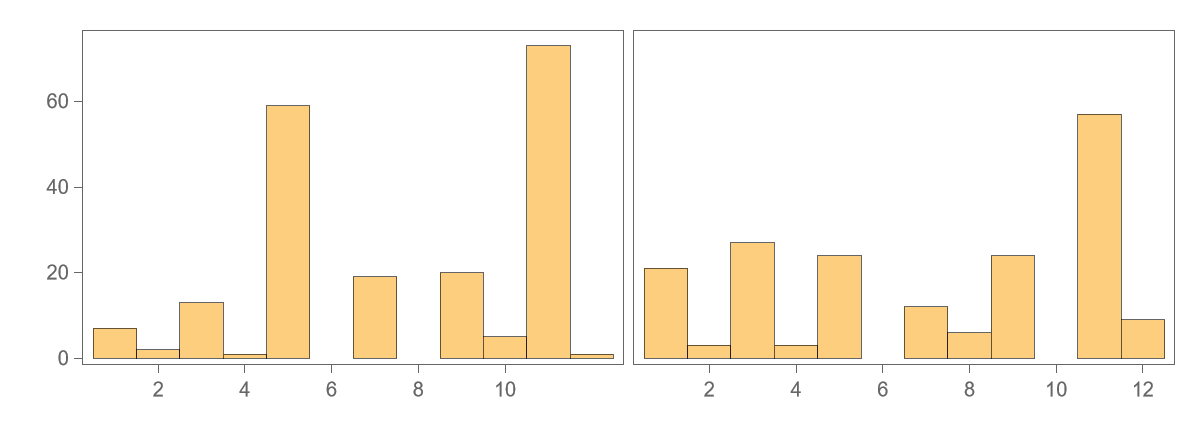
\includegraphics[scale=0.55]{fig/anatomy200.png}
	\caption{An example illustrating anatomy of successful AC paths found by an RL agent in different runs working on different datasets, both of which contain the same hard instance. Even though the total number of moves can vary, e.g. in this example we had to rescale one of the distributions by a factor of 3, curiously, the proportion of moves and combinations used are quite similar. In both cases, RL agents used the same opening move.}
	\label{fig:anatomy200}
\end{figure}

In the following sections we explore the anatomy of successful AC paths further using the tools of unsupervised learning and topological data analysis. These tools offer a complementary perspective on hard-to-find AC paths and ways to find them.

	% !TEX root = ../ac_paper.tex

\section{Language Modeling} \label{sec:lm}

In this section, we discuss a model for the ``language" of balanced presentations.
Each presentation with two relators is a sequence made of six letters, also known as ``tokens" in the nomenclature of Natural Language Processing, i.e. $x$, $y$, $x^{-1}$, and $y^{-1}$, and two ``stop tokens": one that separates two relators of a presentation and another that marks the end of a presentation.
Given this vocabulary $V$ of six tokens, we can ask what is the probability $p(t_1, \dots, t_N)$ for $t_i \in V$ of the occurrence of a specific presentation in the space of all balanced presentations.
Using the chain rule of probability theory,
\[
p(t_1 \cdots t_{N}) = \prod \limits_{i=1}^{N} p (t_{i} \mid t_{1} \cdots t_{i-1})
\]
Here $p (t_{N} \mid t_{1} \cdots t_{N-1})$, often called the $N$-gram probability distribution, is the probability of a token $t_N$ following a sequence of tokens $t_{1} \cdots t_{N-1}$.
To model the language of balanced presentations, we can alternatively estimate the $N$-gram probability distributions for all $N$.

Over the last few years, Transformer models have shown great success in modeling human-understandable languages to the extent that these models can create text almost indistinguishable from that of a human expert.
Specifically, the architecture used for modeling language is the auto-regressive ``decoder-only" Transformer, which we review in detail in \autoref{sec:transformer_review}.
In \autoref{sec:transformer_datasets}, we discuss the method with which we generate the dataset required for training the model.
Finally, in \autoref{sec:transformer_results}, we share details of some insights we learned from this process.

\subsection{Transformers: a review\label{sec:transformer_review}}

Here, we give a short review of the architecture of a decoder-only transformer.
For more details, see \cite{vaswani2023attention, elhage2021mathematical, douglas2023large}.

Given an input sequence $t_1, t_2, \dots, t_{N}$, a decoder-only transformer predicts the probability distribution $p(t \mid t_1, t_2, \dots, t_{N})$ over the set $V$ of tokens of size $n_{\text{vocab}}$.
The probability is computed by applying the softmax function to the logits $T(t)$, which are estimated by applying the following sequence of operations.\footnote{
The softmax function, $\softmax \colon \R^n \to (0, 1)^{n}$, is defined as $\softmax(x)_i = e^{x_i} / \sum\limits_{j=1}^n e^{x_j}$.}
First, assign to each token in the vocabulary a distinct label in the range $1, 2, \dots, n_{\text{vocab}}$; re-writing the original sequence as a sequence of integers.
We will label these integers also as $t_i$.
Next, write the sequence in terms of ``one-hot encoded vectors", i.e. a matrix $t \in \R^{N \times n_{\text{vocab}}}$ such that
\[
t_{ij} = \delta_{i t_i}
\]
and embed the sequence in a $\dm$-dimensional vector space,\footnote{
Here, $t$ and all $x_j$ are two-dimensional tensors.
Hence, it is appropriate to apply tensors of linear transformations to them.
Often in a transformer architecture, these operations are of the form $\mathbb{1} \otimes \cdots$; in these cases, we drop the identity transformation and simply write the operation as $\cdots$.
For example, $\mathbb{1} \otimes W_U$, $\mathbb{1} \otimes W^m_I$, $\mathbb{1} \otimes W^m_O$, etc.
In this case, we will sometimes write $W_U$, $W^m_I$, $W^m_O$ respectively, assuming it is clear from the context and the dimensionality of these matrices that they are tensored with identity transformations.}
\[
x_0 = (W_P \otimes \mathbb{1} + \mathbb{1} \otimes W_E) t
\]
Here, $W_P \in \R^{\dm \times N}$ and $W_E \in \R^{\dm \times n_{\text{vocab}} }$ are matrices of learnable parameters, known as the ``positional embedding" and ``token embedding" matrices.

An $L$-layer transformer alternates between applying a ``multi-head attention layer" ($\sum\limits_{h \in H} h$) and an ``MLP-layer" ($m$) $L$ times.
For $i=0, \dots, L-1$,
\[
\begin{aligned}
	x_{2i+1} &= x_{2i} + \sum_{h \in H} h(\LN(x_{2i})), \\
	x_{2i + 2} &= x_{2i + 1} + m(\LN(x_{2i + 1})).
\end{aligned}
\]
Each $x_j$ is an element of $\mathbb{R^{N \times \dm}}$, with the interpretation that its $i$-th row is the embedding of the sequence $t_1, \dots, t_i$ in the embedding space $\R^{\dm}$ as learned by the preceeding $j+1$ operations.
Finally, one applies an ``unembedding layer", $W_U \in \R^{n_{\text{vocab}} \times \dm}$, to convert the output of the final layer to an $n_{\text{vocab}}$-dimensional vector of logits that estimate the sought-after probability distribution.
\[
\begin{aligned}
	T(t) &= W_U x_{2L-1}, \\
	p(t) &=\softmax (T(t)).
\end{aligned}
\]

The functions $\LN$, $m$ and $h$ are defined as follows.
$\LN$ is the LayerNorm operation that normalizes the input of each layer to make the optimization process more stable~(\cite{ba2016layer}):
\[
\LN(x) = \left(\mathbb{1} \otimes \text{diag}(\gamma) \right) \frac{(x-\overline{x})}{\sqrt{\text{var}(x)}} + \mathbb{1} \otimes \beta\,.
\]
Here, $\overline{x}$ and $\text{var}(x)$ are mean and variance of each row of $x$, and $\gamma, \beta \in \R^{\dm}$ are learnable parameters.
The MLP-layer $m$ is a non-linear operation,
\[
m(x) =W ^m_O \ \max(W_I^m x, 0)
\]
with learnable parameters $W^m_I \in \R^{d_{\text{MLP}} \times \dm}$, $W^m_O \in \R^{\dm \times d_{\text{MLP}}}$.
It is standard to set $d_{\text{MLP}} = 4 \dm$.

Finally, the multi-headed attention-layer $\sum_{h \in H} h$ is a sum of $n_{\text{heads}}$ ``attention-head" operations $h$, where
\[
h(x) = (A^h(x) \otimes W^h_O W^h_V) x.
\]
Here, $W^h_V \in \R^{d_{\text{head}} \times \dm}$,
$W^h_O \in \R^{\dm \times d_{\text{head}}}$
are matrices of learnable parameters;
$d_{\text{head}}$ is the ``attention-head dimension" that satisfies $d_{\text{head}} \times n_{\text{head}} = d_{\text{model}}$; and the attention matrix $A^h$ is computed with the help of learnable matrices
$W^h_Q, W^h_K \in \R^{d_{\text{head}} \times \dm}$,
\[
A^h(x) = \softmax^\star \left(\frac{x^T (W^h_Q)^T W^h_K x}{\sqrt{d_{\text{head}}}}\right).
\]
The attention-head is an $N \times N$ matrix, with the interpretation that $A^h(x)_{ij}$
is the ``attention" paid to the token
$t_j$ in estimating
$p(t_{i+1} \mid t_1, \dots, t_i)$.
$\softmax^\star$ is a variant of the $\softmax$ function suitable for auto-regressive tasks: it sets the upper triangular part of its input to zeros before applying the
$\softmax$ operation.
That is, future tokens, $t_k$ for $k > i$, play no role in the prediction of $p(t_{i+1} \mid t_1, \dots, t_i)$.

We train the transformer model by minimizing the cross-entropy loss between the distributions of predicted and correct labels for the next tokens in a sequence.
The parallelism offered by the processing of all tokens in a sequence at once is extremely beneficial for efficient training of the model for the language modeling task.

In practice, the embedding matrix $W_E$ and the unembedding matrix $W_U$ are often ``tied" together, i.e. $W_E = W_U^T$ \cite{press2017using, inan2017tying}.
The rows of $W_E = W_U^T$ are interpreted as the embeddings of words/sentences, to which one may apply the usual operations of a vector space \cite{Bengio:2003, mikolov-etal-2013-linguistic}.
For example, the cosine of the angle between two embedding vectors, also known as the ``cosine similarity", is often used to measure the similarity between two texts.
Two semantically similar texts have higher cosine similarity between them, while semantically different texts correspond to (almost) orthogonal vectors in the embedding space.

\subsection{Training and evaluation datasets\label{sec:transformer_datasets}}

We now discuss the training and validation datasets used to train and evaluate our Transformer model.
As our main interest in this paper has been in the presentations of the Miller--Schupp series, we generated a dataset of balanced presentations that are AC-equivalent to the Miller--Schupp presentations.
Specifically, we apply sequences of AC-moves to the 1190 presentations with $n \leq 7$ and $\length(w) \leq 7$ discussed in \autoref{sec:AC}, creating a dataset of about 1.8 million presentations.
Approximately 1 million of these presentations are AC-equivalent to the presentations that remained unsolved by greedy search (c.f. \autoref{sec:search}).
Only a small amount (roughly 15 percent) of the original Miller--Schupp presentations were part of this dataset.

The dataset is tokenized using six tokens: two stop tokens and one token each for the two generators and their inverses.
The tokenized dataset had about $2.17 \times 10^8$ tokens.
As our goal is to get insights into properties that distinguish GS-solved and GS-unsolved presentations, we performed an exploratory data analysis of the two subsets of data associated to these presentations.
We plot the percentage of appearance of each token for these subsets in \autoref{fig:tokens_hist}.
The ratio of frequency of $y^{\pm 1}$ to the frequency of $x^{\pm 1}$ is higher in the GS-unsolved dataset.
This is likely because the GS-unsolved presentations have larger $n$, and larger $n$ corresponds to a higher number of occurrence of $y^{\pm 1}$ in the Miller--Schupp presentation.
Interestingly, this effect remains in the dataset even after applying thousands of AC-moves to the original presentations.

We paid special attention to ensure that our dataset contains presentations of a wide range of lengths so as not to bias our model towards learning trends specific to any fixed length.
To this end, we devised an algorithm (\autoref{alg:apply_ac_moves} in \autoref{app:algorithm}) that creates an almost uniform distribution over the lengths of the presentations.
(See \autoref{fig:gpt_data}.) We set aside $10\%$ of our entire data for validation.

\begin{figure}
	\centering
	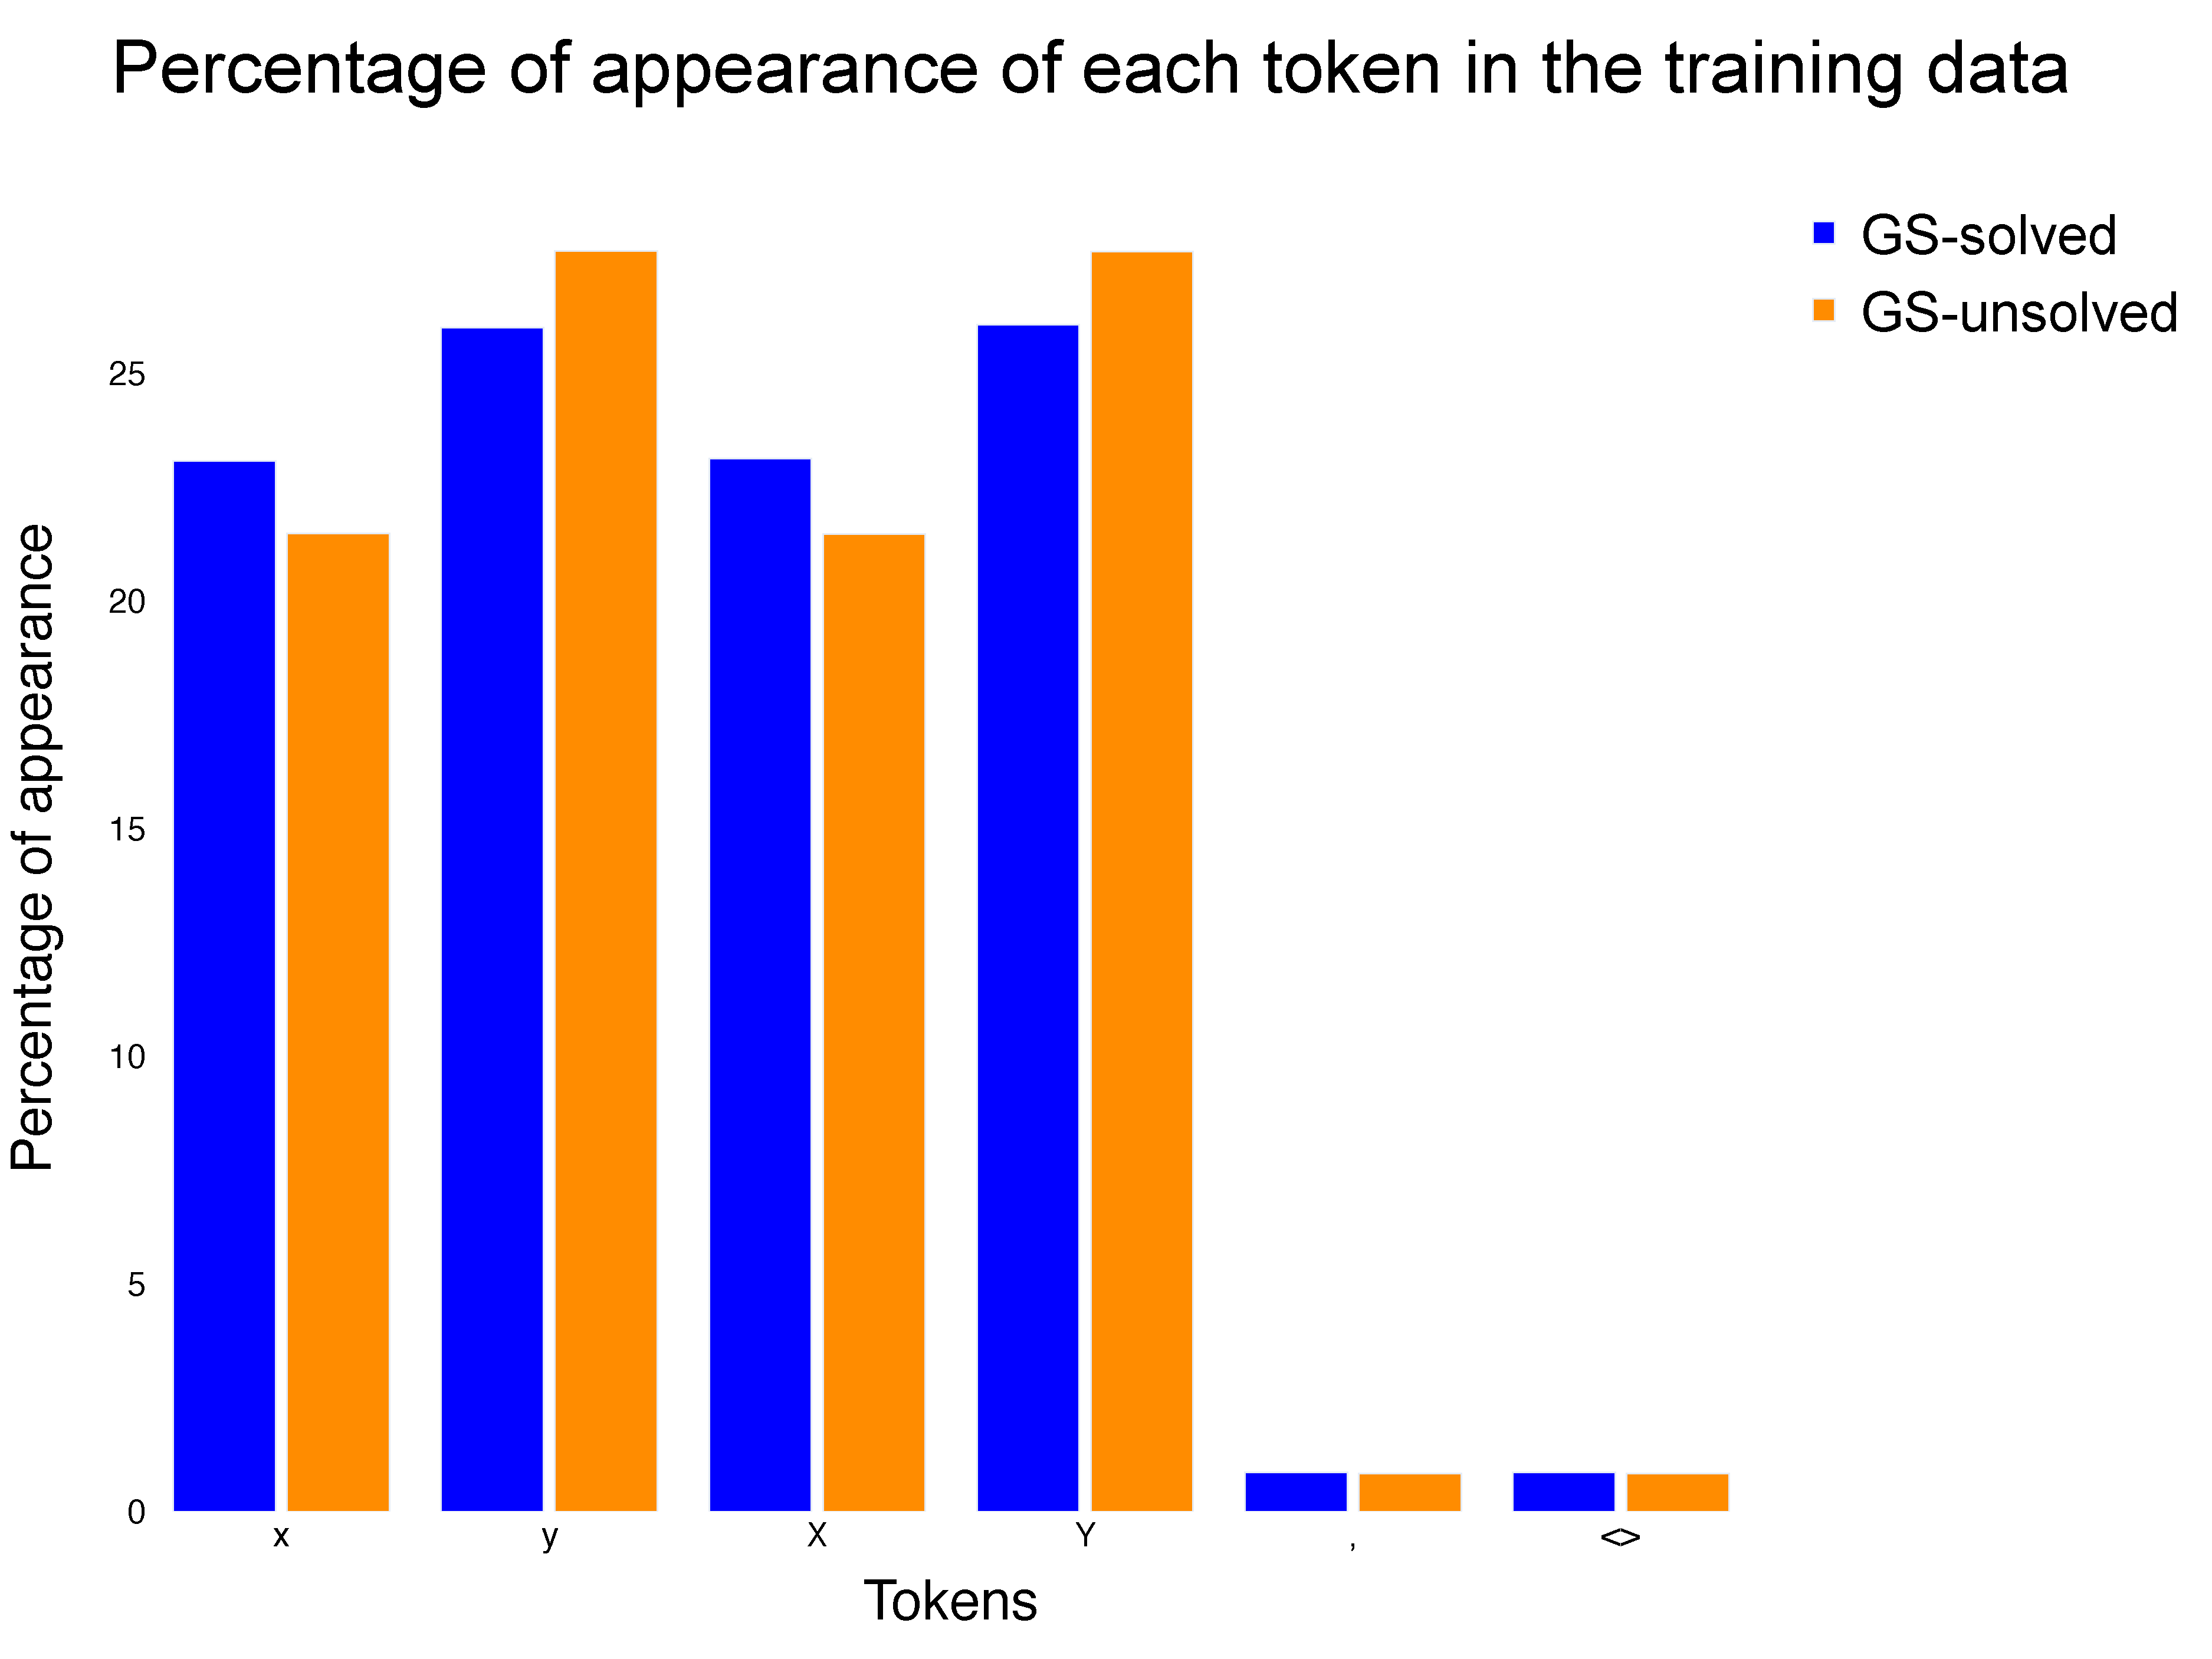
\includegraphics[scale=0.15]{fig/tokens_hist.pdf}
	\caption{Percentage of appearance of each token in the two subsets of the training dataset that are equivalent to GS-solved and GS-unsolved presentations.
	To be clear, we computed the percentages separately for each subset of the training data, i.e. the heights of all blue (and orange) bars adds separately to 100.}
	\label{fig:tokens_hist}
\end{figure}

\begin{figure}
	\centering
	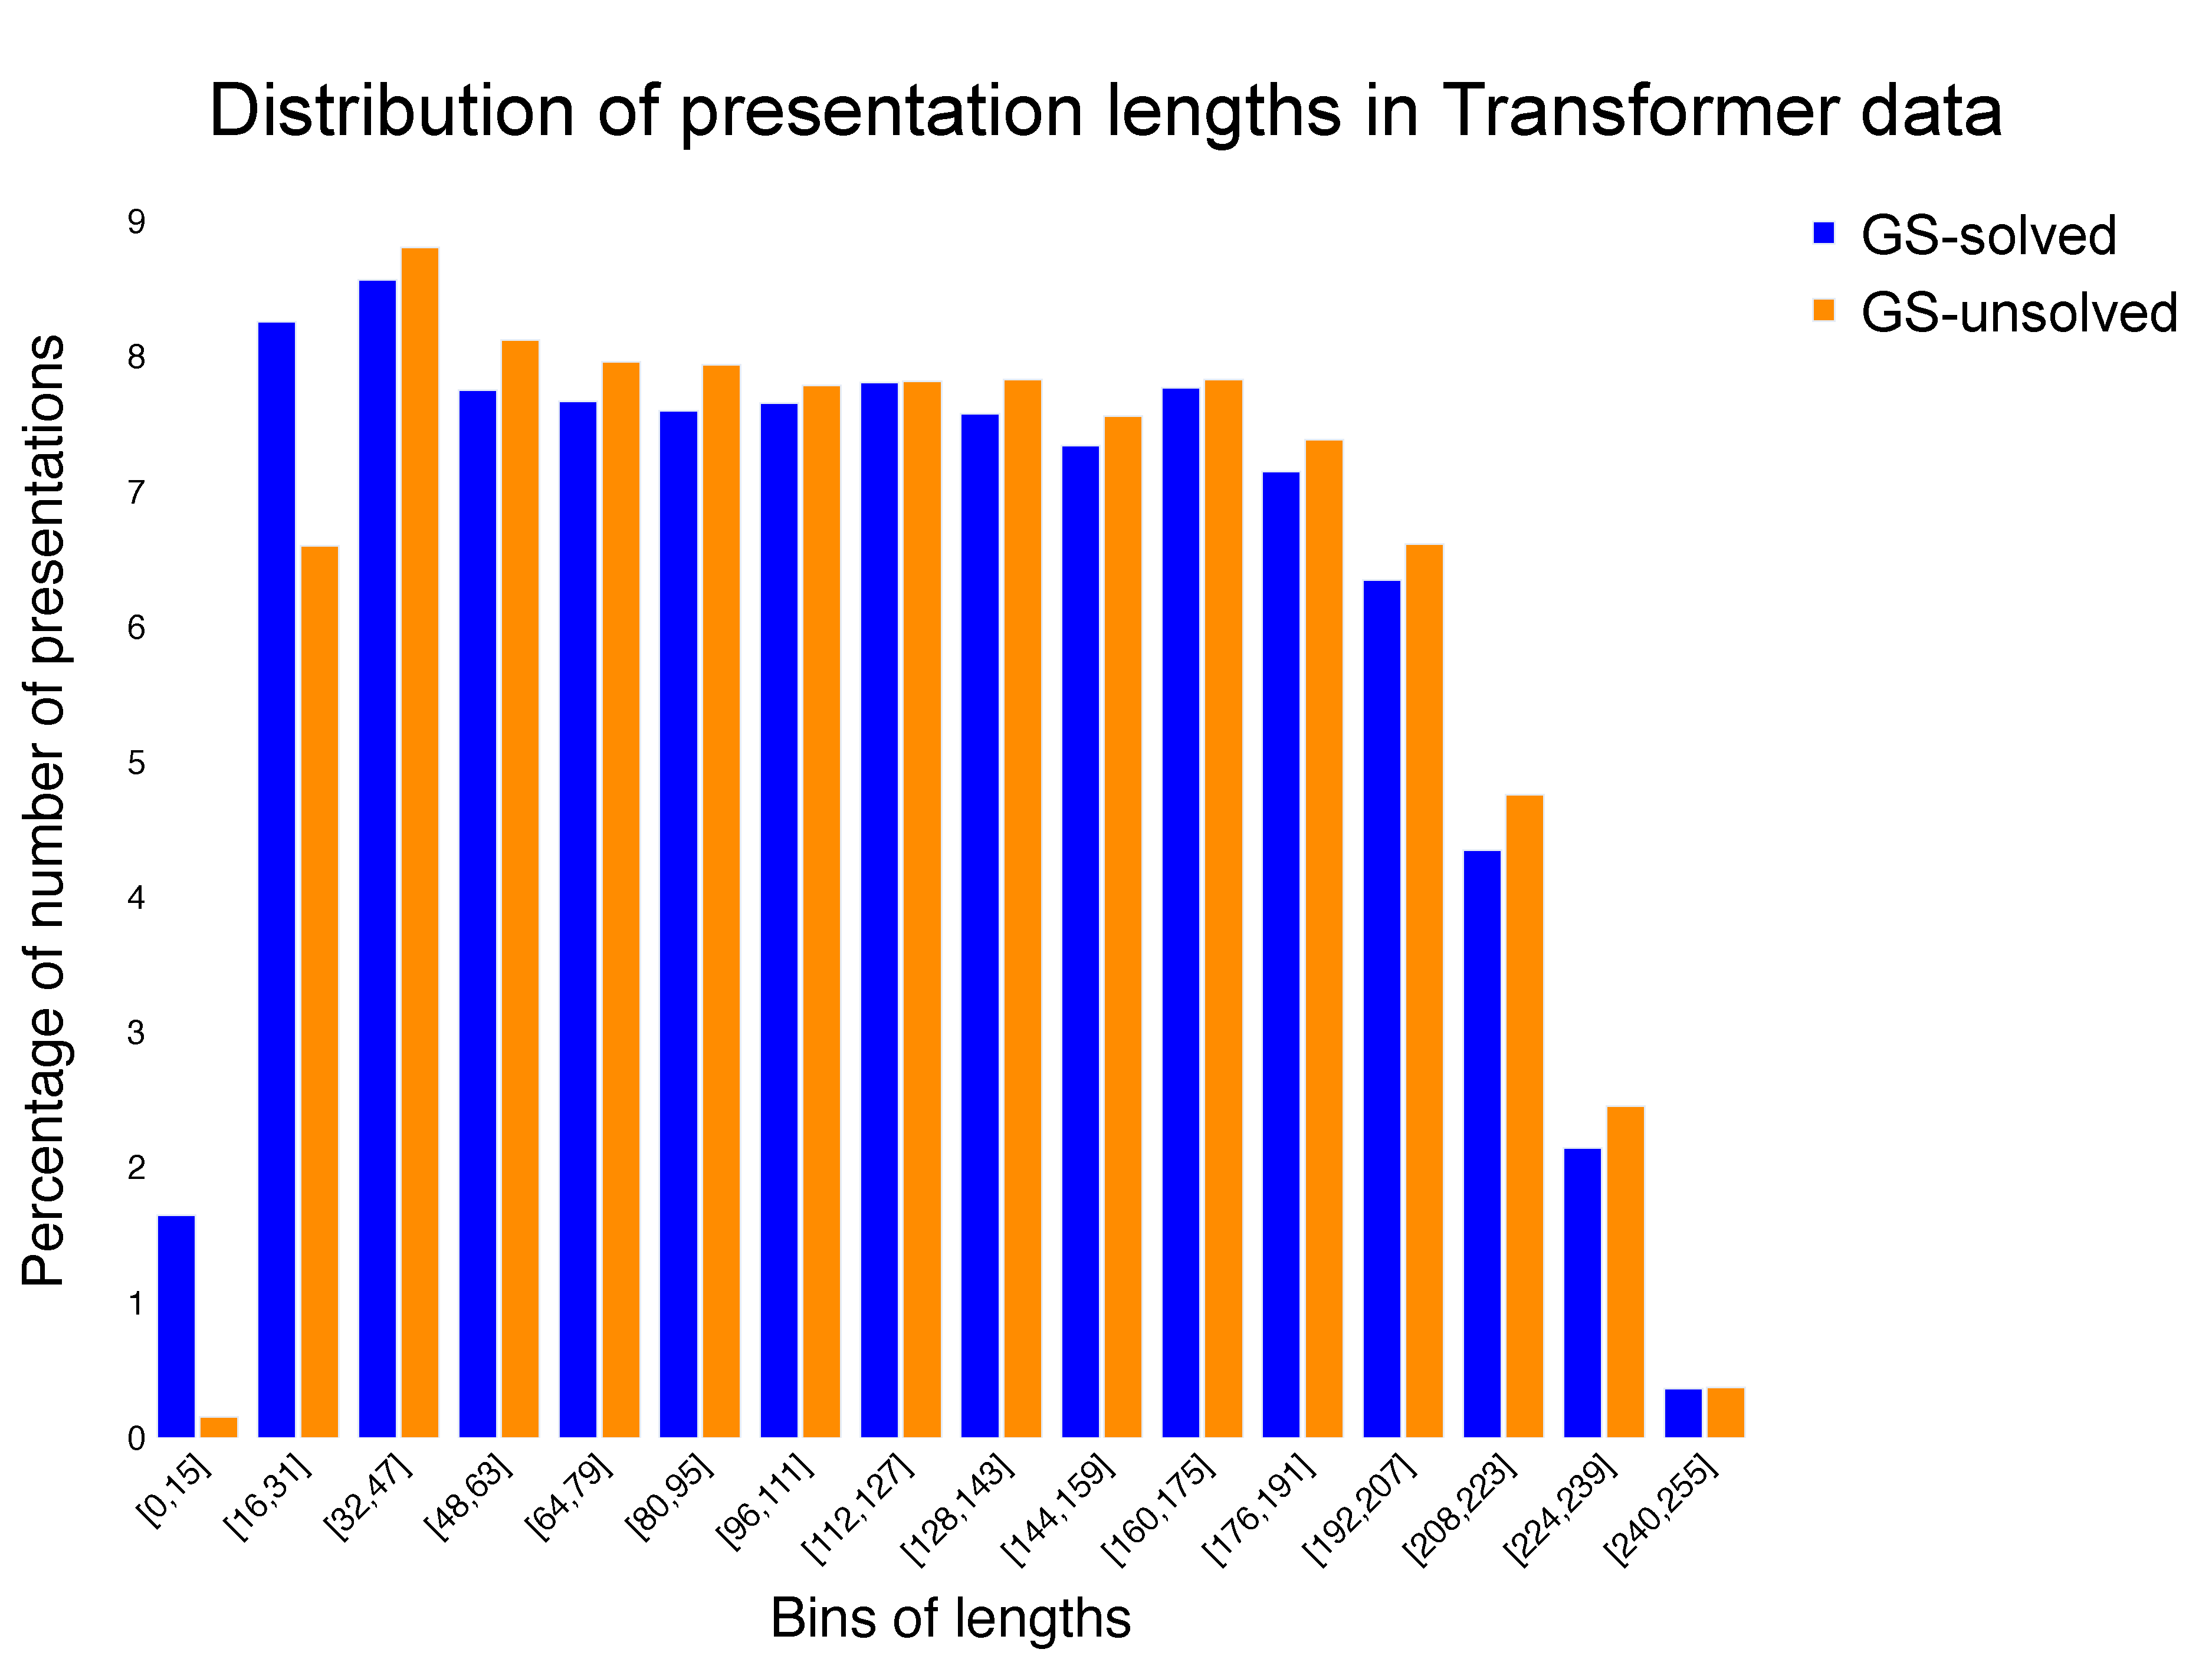
\includegraphics[scale=0.15]{fig/gpt_data_length_distribution.pdf}
	\caption{Percentage of presentations in various ranges of lengths.
	Percentages were computed independently for the two subsets of the dataset, corresponding to presentations that are AC-equivalent to GS-solved and GS-unsolved presentations.
	We used \autoref{alg:apply_ac_moves} from \autoref{app:algorithm} to ensure the almost-uniform distribution depicted here.}
	\label{fig:gpt_data}
\end{figure}

\subsection{Results}\label{sec:transformer_results}

A randomly initialized model with the initialization scheme given in \cite{Radford2019LanguageMA} has a cross entropy loss of
%$- \ln \left(\frac{1}{n_{\text{vocab}}} \right) \approx - 1.7918$,
$-\ln (1/n_{\text{vocab}}) \approx 1.7918$.
With training, we could achieve a validation loss of $0.7337$.\footnote{
We tuned the hyperparameters a little but it is quite likely that one can achieve a better performing model with more hyperparameter tuning.
Similarly, more training data will necessarily help with the performance.
We trained a Transformer model with hyperparameters given in \autoref{app:hyperparameters}.}
We used the untrained and the trained model to get the embeddings of all $1190$ presentations of the Miller--Schupp series with $n \leq 7$ and $\length(w) \leq 7$.
We used t-SNE to project these embedding vectors to a plane \cite{JMLR:v9:vandermaaten08a}.
The plots are shown in grid in \autoref{fig:tsne_embeddings}.

Each row of \autoref{fig:tsne_embeddings} corresponds to a fixed value of $n$.
The left (resp. right) column depicts t-SNE projections of embeddings obtained by an untrained (resp. trained) model.
t-SNE dependence on a distance measure: it learns to map vectors that are closer together in the higher-dimensional space, with respect to this distance measure, close together in the plane \cite{JMLR:v9:vandermaaten08a}.
We used cosine simiarity between embedding vectors as the distance measure for our plots.
We note that the GS-solved and GS-unsolved presentations seem to cluster much more in the plots in the right column.
This indicates that a trained Transformer model is able to distinguish between GS-solved and GS-unsolved presentations to a good extent, albeit not perfectly.\footnote{
Note also that t-SNE admits a hyperparameter known as ``perplexity", and the projections learned by t-SNE depend on the hyperparameter \cite{wattenberg2016how}.
Thus, in general, t-SNE plots must be interpreted with care.
The plots shown in \autoref{fig:tsne_embeddings} were all made with the perplexity value of $30$.
We checked however that the clusters of GS-solved and GS-unsolved presentations continue to exists at a broad range of perplexity values.}

Note that the training dataset contained no information about the ease of solvability of a presentation.
It also did not contain many presentations of the Miller--Schupp series itself.
Instead, it contained presentations that are AC-equivalent to the Miller--Schupp series presentations.
Our observation that a Transformer model trained on this dataset can distinguish between the GS-solved and GS-unsolved presentations indicates that:
\begin{enumerate}[label=\alph*)]
	\item There likely exists an invariant at the level of the ``language" of the balanced presentations that distinguishes GS-solved vs GS-unsolved presentations.
	\item This invariant survives application of thousands of AC-moves we used to generate the training examples in our dataset.
\end{enumerate}

\begin{figure}
	\centering
	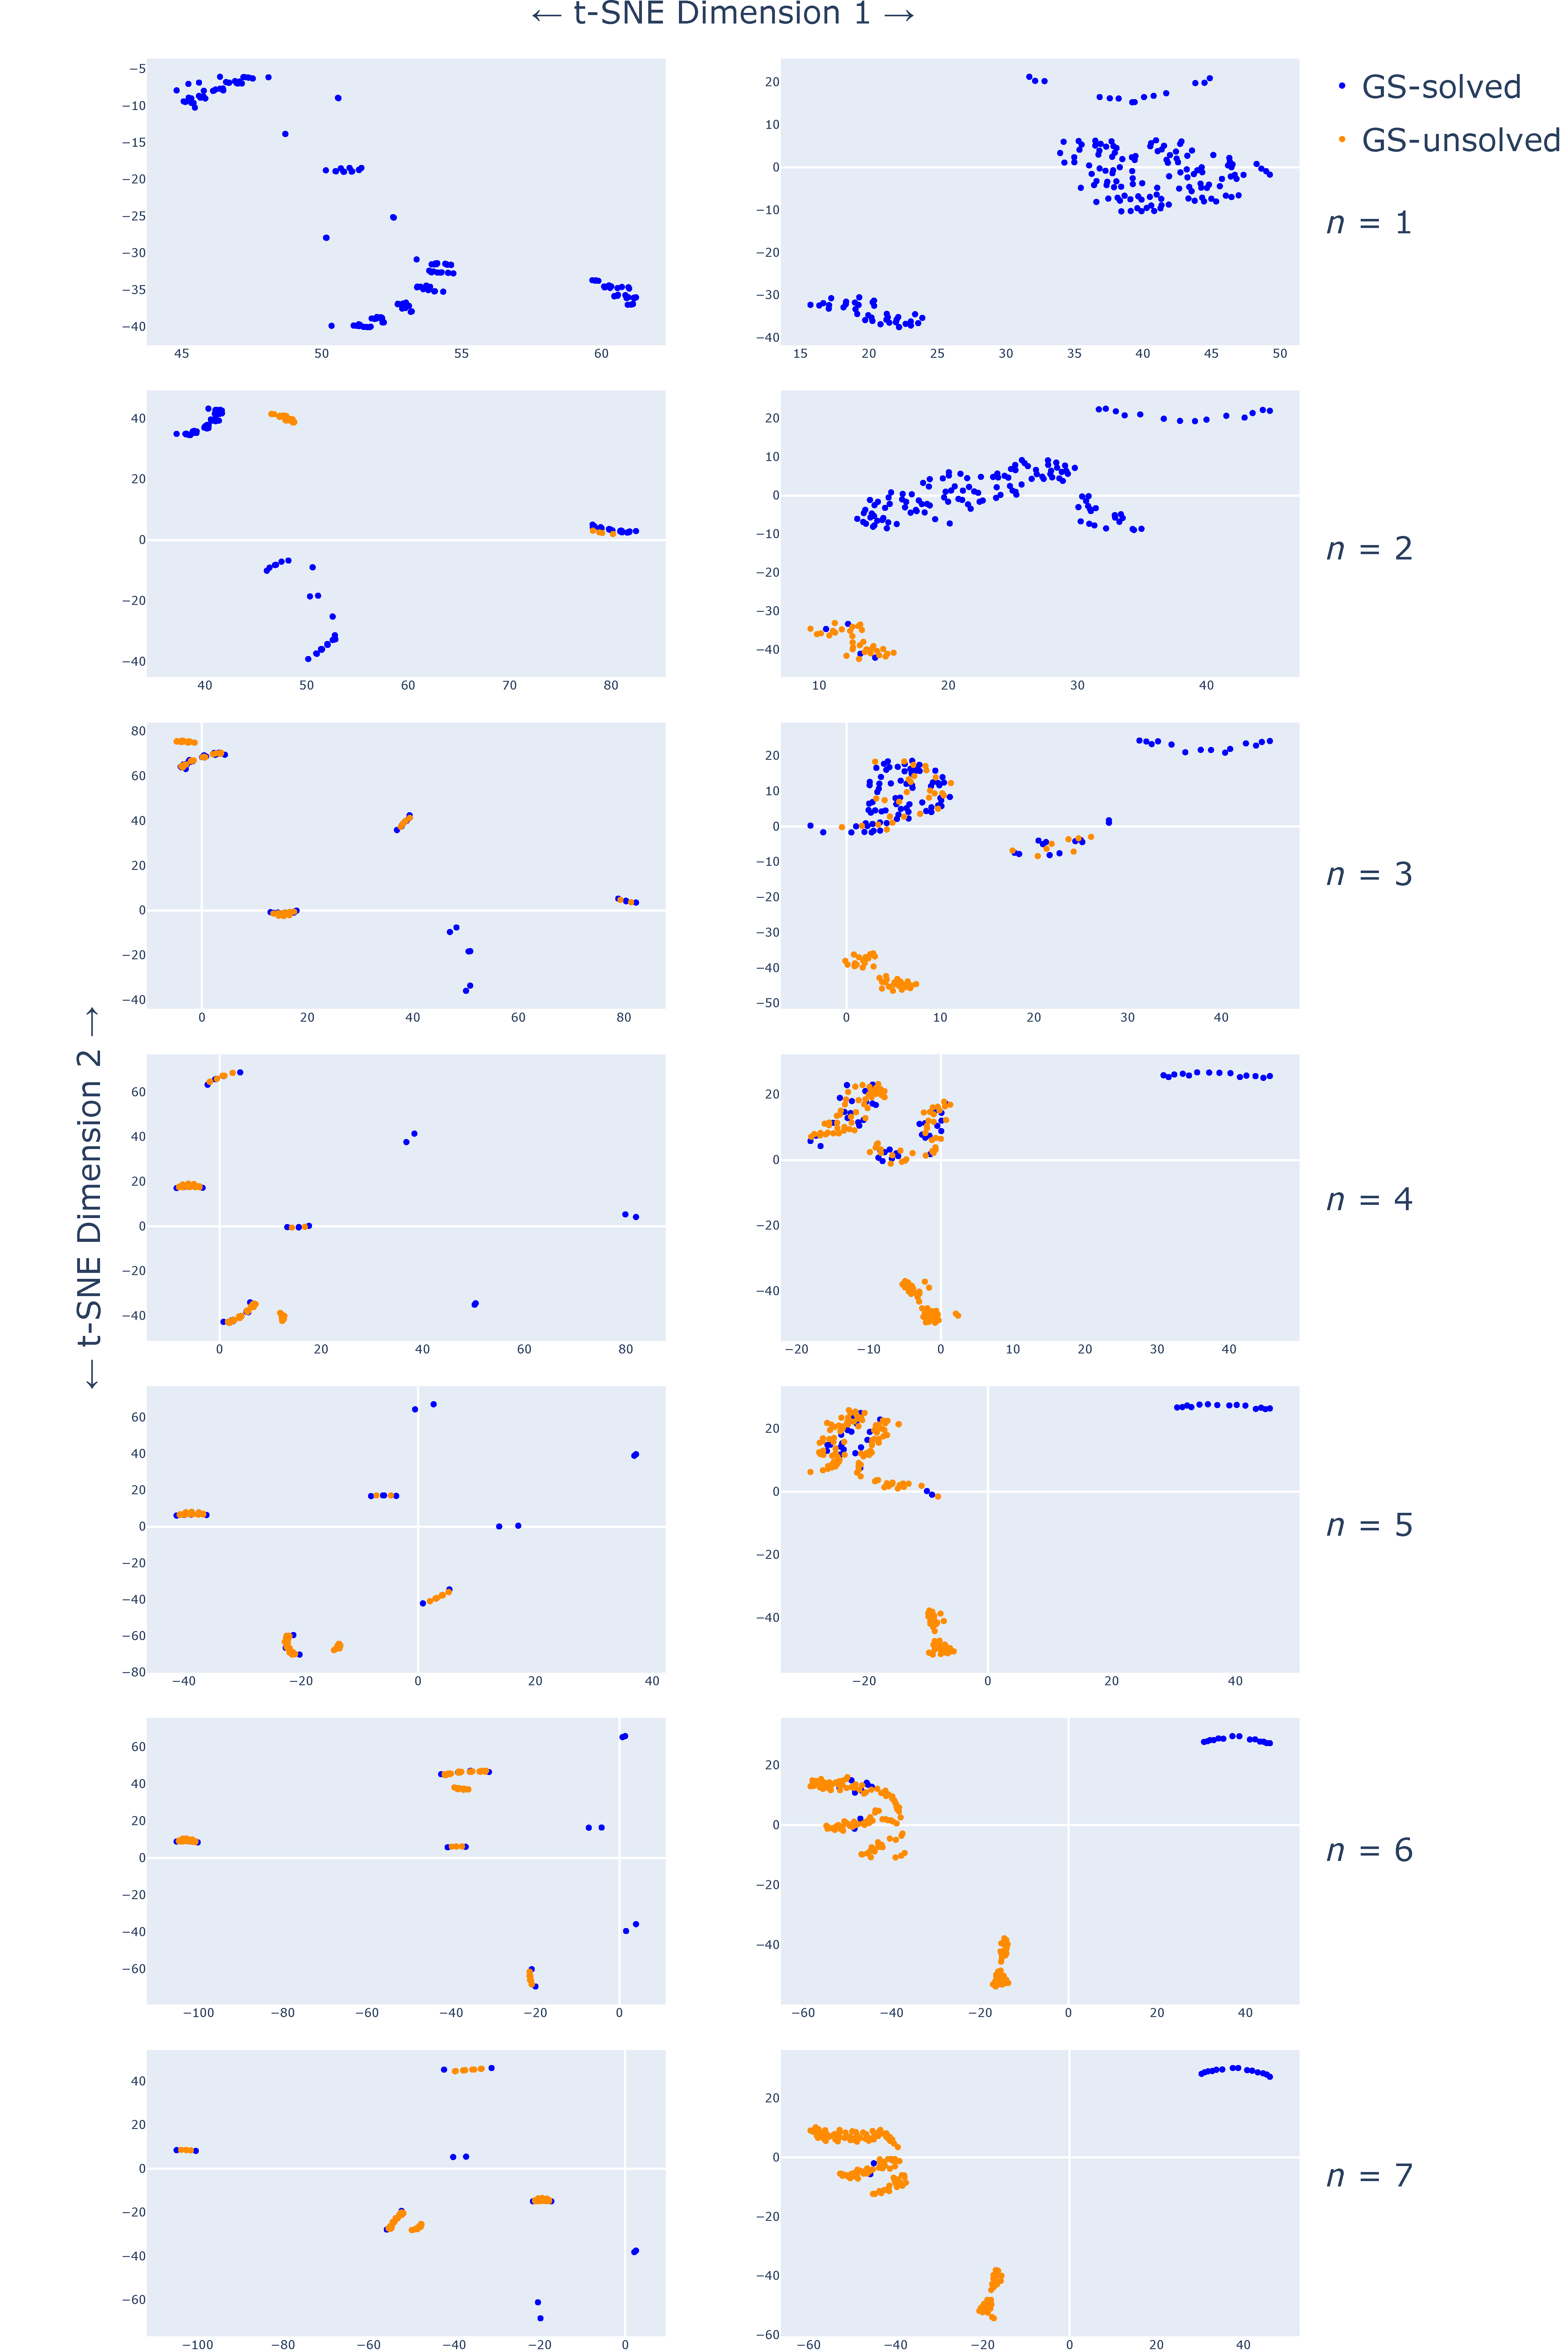
\includegraphics[scale=0.16]{fig/embeddings.pdf}
	\captionsetup{width=1.1\textwidth}
	\caption{t-SNE plots depicting embeddings of the Miller--Schupp presentations $MS(n, w)$.
	The left (right) column shows embeddings learned by an untrained (trained) transformer model.
	Each row corresponds to a value of $n$.
	Trained models cluster together GS-solved and GS-unsolved presentations indicating the possibility of a difference in the linguistic structure of the two sets of presentations.}
	\label{fig:tsne_embeddings}
\end{figure}

	% !TEX root = ../ac_paper.tex

\section{Neighborhood sizes and isolated components}\label{sec:isolated}

\subsection{Neighborhoods}

Let us return to our data set of 1190 presentations in the Miller--Schupp series for \(n \leq 7\) and \(\length(w) \leq 7\).
Using the methods described in \autoref{sec:ppo}, we trained a PPO agent that successfully solved 417 of these presentations.
We will refer to the set of these 417 presentations as PPO-solved and the remaining 773 presentations as PPO-unsolved.
Our goal is to analyze the relationship between these labels and the sizes of their respective AC neighborhoods.
A presentation is considered to be in the \(k\)-step neighborhood of another if they can be connected by applying at most \(k\) AC-moves.

\subsubsection{Experimental results}

There are 131 distinct neighborhood sizes in our data.
Their basic statistics are
\[
\begin{tabular}{cccccc}
	\toprule
	\textbf{Min} & \textbf{Max} & \textbf{Mean} & \textbf{Median} \\
	\midrule
	72,964 & 89,872 & 89,532 & 89,859 \\
	\bottomrule
\end{tabular}
\]
A more detailed description of the frequency of values is presented in \autoref{fig:prime_combined_pie}.

\begin{figure}
	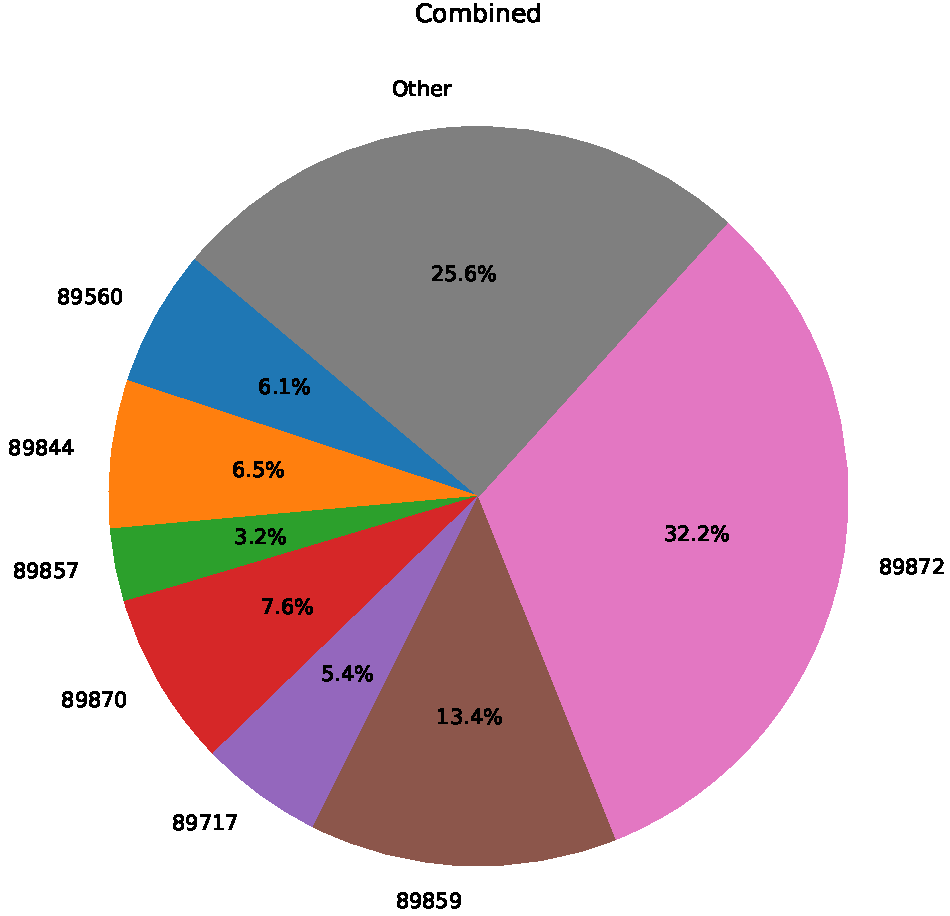
\includegraphics[scale=.4]{fig/prime_combined_pie_rl_cropped.pdf}
	\caption{Sizes of the 5-step neighborhood of all considered presentations in the Miller--Schupp series. We group neighborhood sizes whose representation is below 2.5\%.}
	\label{fig:prime_combined_pie}
\end{figure}

The largest neighborhood size accounts for nearly a third of all considered presentations.
However, it represents only 2.4\% of PPO-solved presentations, while constituting almost half (48.3\%) of the PPO-unsolved presentations.
For more details, please refer to \autoref{fig:prime_pies}.

In contrast, using BFS, these proportions are 7.1\% and 52.5\%, respectively.

Another notable feature visible in \autoref{fig:prime_pies} is that just three neighborhood sizes account for over three-quarters of all PPO-unsolved presentations.
When considering six neighborhood sizes, this proportion rises to 96.9\%.
In fact, only twelve neighborhood sizes are present among PPO-unsolved presentations, whereas all 131 sizes appear among PPO-solved presentations.
The most common neighborhood size for PPO-solved presentations is 89,560, representing only 17.3\% of them.
Moreover, 54.2\% of all PPO-solved presentations have a neighborhood size shared by less than 2.5\% of other PPO-solved presentations.

\begin{figure}
	\centering
	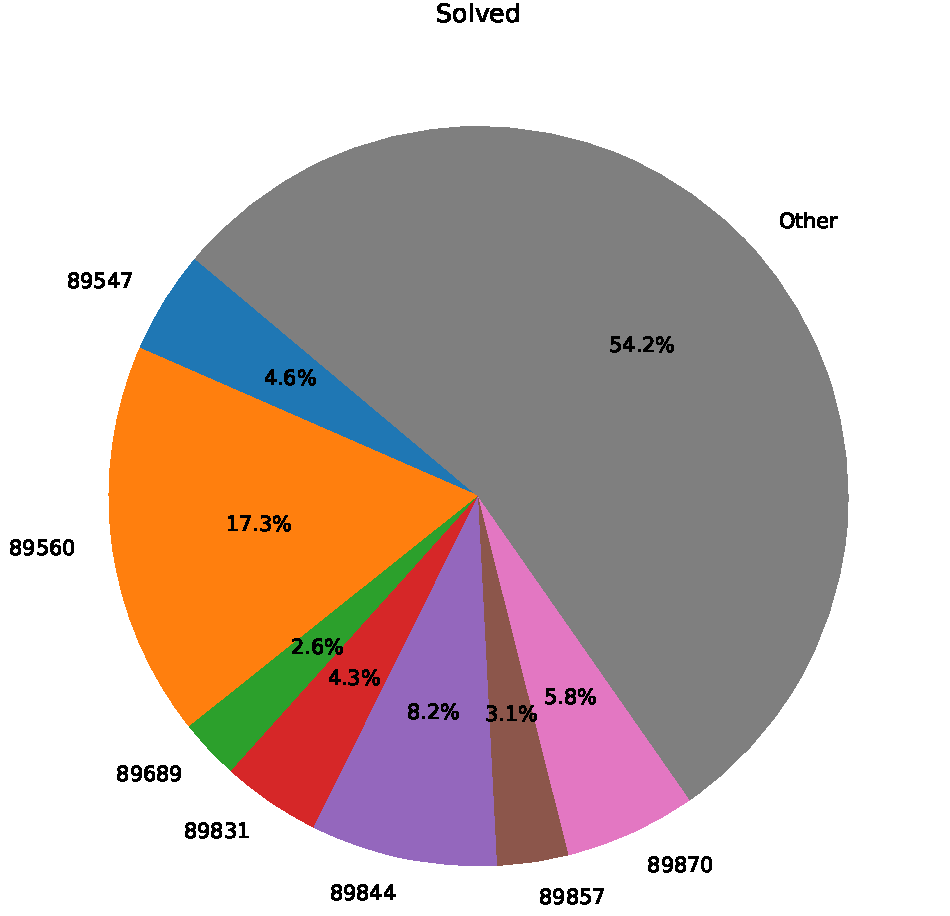
\includegraphics[scale=.35]{fig/prime_solved_pie_rl_cropped.pdf}
	\
	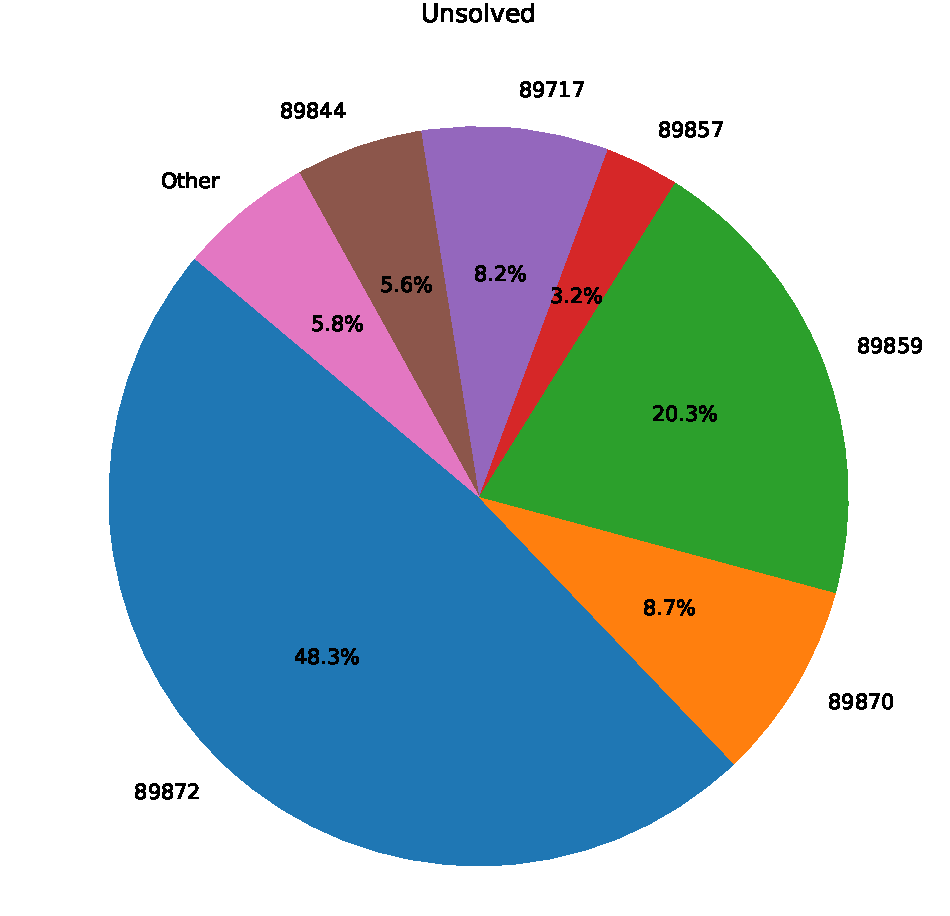
\includegraphics[scale=.35]{fig/prime_unsolved_pie_rl_cropped.pdf}
	\caption{Pie charts for the neighborhood size of PPO-solved and PPO-unsolved presentations. We grouped sizes with representation below 2.5\%.}
	\label{fig:prime_pies}
\end{figure}

As we observed, having a maximal neighborhood size provides significant insight into whether a presentation is labeled as PPO-solved or PPO-unsolved.
Additionally, the minimum neighborhood size among PPO-unsolved presentations—89,573—is also quite telling, as 54\% of PPO-solved presentations have neighborhood sizes smaller than this value.
This percentage can be further improved by considering that the neighborhood sizes of PPO-unsolved presentations are concentrated within three specific bands.
Please refer to \autoref{fig:prime_histogram} for more details.
We find that 64.3\% of PPO-solved presentations fall outside the three bands \([89,575, 89,575]\), \([89,715, 89,831]\), and \([89,844, 89,872]\), which together contain over 99\% of PPO-unsolved presentations.
By narrowing the last band to \([89,859, 89,872]\), these three bands now encompass the neighborhood sizes of over 90\% of PPO-unsolved presentations, while their complement includes 77.2\% of PPO-solved presentations.

\begin{figure}
	\centering
	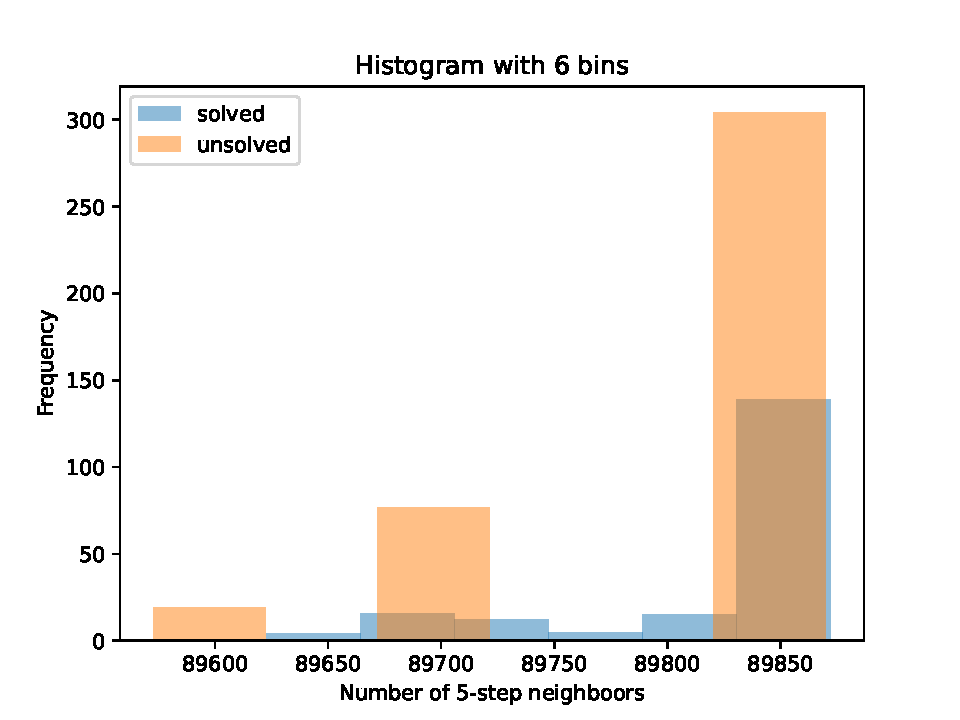
\includegraphics[scale=.34]{fig/prime_histogram_rl.pdf}
	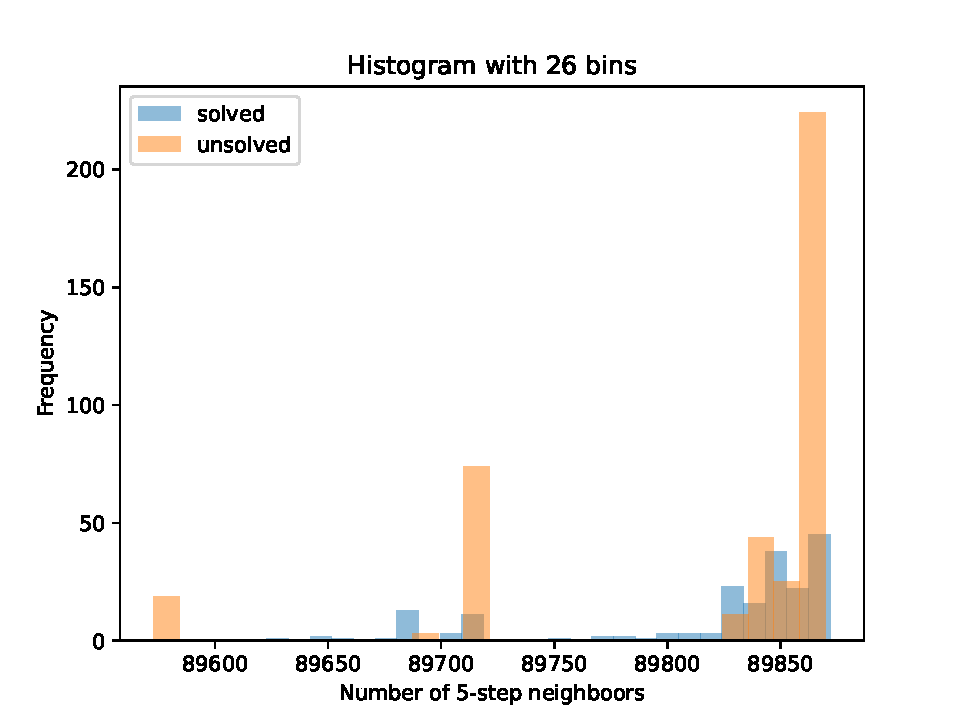
\includegraphics[scale=.34]{fig/prime_histogram_rl2.pdf}
	\caption{Histograms with 6 and 26 bins respectively of the neighborhood sizes of the 417 PPO-solved and 773 PPO-unsolved presentations.}
	\label{fig:prime_histogram}
\end{figure}

\medskip

One might expect that enhancing the discriminatory power of \(n\)-neighborhoods could be achieved by incorporating features beyond their size.
We explored two additional types of features, but surprisingly, they only marginally improved the accuracy of PPO-solved/unsolved predictions.
The first type was based on node centrality, while the second focused on spectral features of the neighborhood graphs.
The latter was particularly intriguing, given the emphasis on Markov processes and the well-known relationship between random walks on graphs and the graph Laplacian.


\subsection{Isolated components}

In \autoref{ss:greedy_search}, we explored a greedy approach to finding AC-trivializations of a presentation \(\pi\).
Specifically, the goal was to construct a sequence of presentations \((\pi_0, \dots, \pi)\), where \(\pi_0\) is the trivial presentation, such that each consecutive pair in the sequence is related by an AC-move.
Furthermore, at each step \(k\), the presentation \(\pi_k\) was chosen to have the shortest possible length among all presentations connected to \(\pi_{k+1}\) via an AC-move.
In general, the length of a presentation in an AC-trivialization tends to exceed the length of the original presentation being trivialized.
The minimum increase in length across all possible AC-trivializations serves as an invariant of the presentation.
We will explore this invariant using concepts from persistent homology.

\subsubsection{Formalization}

A \textit{based graph} is a pair $(\Gamma, v_0)$ consisting of a graph $\Gamma$ and a preferred vertex $v_0$ in it.
We will often drop $v_0$ from the notation.
A \textit{based subgraph} $\Gamma_n$ of $\Gamma$, written $\Gamma_n \leq \Gamma$, is a subgraph $\Gamma_n$ of $\Gamma$ with the same preferred vertex.
We say that $\Gamma_n$ is \textit{full} in $\Gamma$ if for any two vertices in $\Gamma_n$ joined by an edge in $\Gamma$, the edge is also in $\Gamma_n$.
A \textit{filtration} of a based graph $\Gamma$ is a collection
\[
\Gamma_0 \leq \Gamma_1 \leq \Gamma_2 \leq \dotsb
\]
of based subgraphs of $\Gamma$ for which each vertex and edge of $\Gamma$ is in $\Gamma_n$ for some $n$.
We refer to $\Gamma$ as a \textit{filtered based graph}.
If each $\Gamma_n$ is full in $\Gamma$ we refer to the filtration as full and notice that full filtrations are equivalent to $\N$ valued functions from the set of vertices of $\Gamma$ sending $v_0$ to $0$.

Let $\Gamma^{\text{AC(k)}}$ be the graph whose vertices are $k$-balanced presentations, based at the trivial presentation, having an edge between two vertices if there is an AC-move between them.
Additionally, $\Gamma^{\text{AC(k)}}$ is equipped with a full filtration obtained from the function sending a vertex to the length of its presentation minus $k$.

%\subsubsection{Isolation values and isolated components}

Given a filtered based graph $(\Gamma, v_0)$.
The \textit{filtration value} $\Filt(v)$ of a vertex $v$ is the smallest $n \in \N$ such that $v$ is a vertex in $\Gamma_n$.
Similarly, its \textit{connectivity value} $\Conn(v)$ is the smallest $n \in \N$ such that $v$ and $v_0$ can be joined by a path in $\Gamma_n$ or is set to $\infty$ if such path does not exist in $\Gamma$.

The \textit{isolation value} of a vertex $v$ in a filtered based graph is defined as
\[
\Isol(v) = \Conn(v) - \Filt(v),
\]
a number in $\N \cup \set{\infty}$.
A vertex is said to be \textit{isolated} if its isolation value is positive.

We introduce an equivalence relation on isolated vertices.
Two belong to the same \textit{isolated component} if they have the same connectivity value, say $n$, and they can be joined by a path in $\Gamma_{n-1}$.
The \textit{isolation value} of a component is the maximum of the isolation values of its elements.

We can interpret these invariants using the framework of topological data analysis, see for example \cite{carlsson2022tda}.
Specifically, the set of isolated components of a based filtered graph $\Gamma$ corresponds to the multiset of bars in the barcode of its reduced persistent $0$-homology.
Additionally, the isolation value of an isolated component corresponds to the length of its associated bar.

\subsubsection{Experimental results}

Let \(\Gamma^\ell\) be the full subgraph of \(\Gamma^{\text{AC(2)}}\), with the induced filtration, consisting of all presentations with a connectivity value less than or equal to \(\ell\).
Explicitly, \(\Gamma^\ell\) includes all vertices that can be connected to the trivial vertex via paths containing only presentations of length at most \(\ell\).

We will denote by $v(\ell)$ and $e(\ell)$ the number of vertices and edges of $\Gamma^\ell$.
Let us denote by $ic(\ell)_k$ the number of isolated components with isolation value $k$.
\autoref{fig:classical_persistence} summarize our results for the classic AC-moves whereas \autoref{fig:prime_persistence} does so for their prime version.\footnote{For this task we used \texttt{giotto-TDA} version 5.1 \cite{tauzin2021giotto}.
	Specifically, its binding of the \texttt{SimplexTree} data structure introduced in \cite{boissonnat2014simplex} and implemented in \texttt{GUDHI} \cite{maria2014gudhi}.}

\begin{figure}
	\begin{tabular}{|c|c|c|c|c|c|}
		\hline
		$\ell$ & $v(\ell)$ & $e(\ell)$ & $ic(\ell,1)$ & $ic(\ell,2)$ & $ic(\ell,3)$ \\ \hline
		3 & 36 & 72 & 0 & 0 & 0 \\ \hline
		4 & 100 & 248 & 0 & 0 & 0 \\ \hline
		5 & 388 & 1072 & 0 & 0 & 0 \\ \hline
		6 & 884 & 2376 & 0 & 0 & 0 \\ \hline
		7 & 3892 & 10775 & 0 & 0 & 0 \\ \hline
		8 & 9172 & 25675 & 0 & 0 & 0 \\ \hline
		9 & 37428 & 106513 & 0 & 0 & 0 \\ \hline
		10 & 84996 & 239733 & 0 & 0 & 0 \\ \hline
		11 & 350356 & 1002439 & 4 & 0 & 0 \\ \hline
		12 & 791140 & 2251375 & 16 & 0 & 0 \\ \hline
		13 & 3238052 & 9321629 & 72 & 4 & 0 \\ \hline
		14 & 7199908 & 20573343 & 144 & 4 & 0 \\ \hline
		15 & 29243812 & 84391763 & 508 & 52 & 8 \\ \hline
		16 & 64623652 & 185162236 & 1034 & 88 & 20 \\ \hline
	\end{tabular}
	\caption{Classical AC-moves}
	\label{fig:classical_persistence}
\end{figure}

\begin{figure}
	\begin{tabular}{|c|c|c|c|c|c|}
		\hline
		$\ell$ & $v(\ell)$ & $e(\ell)$ & $ic(\ell,1)$ & $ic(\ell,2)$ & $ic(\ell,3)$ \\ \hline
		3 & 36 & 40 & 3 & 0 & 0 \\ \hline
		4 & 100 & 152 & 3 & 0 & 0 \\ \hline
		5 & 388 & 712 & 3 & 0 & 0 \\ \hline
		6 & 884 & 1528 & 3 & 0 & 0 \\ \hline
		7 & 3892 & 6984 & 3 & 0 & 0 \\ \hline
		8 & 9172 & 16728 & 3 & 0 & 0 \\ \hline
		9 & 37428 & 69752 & 3 & 0 & 0 \\ \hline
		10 & 84996 & 155752 & 3 & 0 & 0 \\ \hline
		11 & 350356 & 655928 & 19 & 0 & 0 \\ \hline
		12 & 791140 & 1467080 & 67 & 0 & 0 \\ \hline
		13 & 3238052 & 6107112 & 243 & 16 & 0 \\ \hline
		14 & 7199908 & 13414744 & 483 & 16 & 0 \\ \hline
		15 & 29243812 & 55306744 & 1819 & 136 & 32 \\ \hline
		16 & 64623652 & 120824232 & 3923 & 208 & 80 \\ \hline
	\end{tabular}
	\caption{Prime AC-moves}
	\label{fig:prime_persistence}
\end{figure}

\subsubsection{}

It is natural to base the AC-graph at a potential counterexample to the AC conjecture.
Let \(\Sigma^\ell\) be the full subgraph of \(\Gamma^{\text{AC(2)}}\) containing all presentation that can be joined to \(AK(3)\) through a path whose maximum length is at most \(\ell\).
In \autoref{fig:ak_classic_persistence} and \autoref{fig:ak_prime_persistence} we respectively present the number of vertices, edges, and isolated components of \(\Sigma^\ell\) constructed using classic and prime moves.

\begin{figure}
	\begin{tabular}{|c|c|c|c|c|c|c|c|c|c|}
		\hline
		$\ell$ & $v(\ell)$ & $e(\ell)$ & $ic(\ell,1)$ & $ic(\ell,2)$ & $ic(\ell,3)$ & $ic(\ell,4)$ & $ic(\ell,5)$ & $ic(\ell,6)$ \\ \hline
		15 & 6864 & 20762 & 1 &  &  &  &  &  \\ \hline
		16 & 10280 & 31090 & 4 & 1 &  &  &  &  \\ \hline
		17 & 428904 & 1297682 & 68 & 27 & 2 & 4 &  &  \\ \hline
		18 & 1007496 & 3047669 & 122 & 27 & 10 & 4 &  &  \\ \hline
		19 & 11804992 & 35738752 & 498 & 115 & 30 & 16 & 12 & 1 \\ \hline
		20 & 25705728 & 77795370 & 826 & 147 & 46 & 28 & 32 & 1 \\ \hline
	\end{tabular}
	\caption{Isolated components with respect to base \(AK(3)\) in the AC graph constructed with classic moves.}
	\label{fig:ak_classic_persistence}
\end{figure}

\begin{figure}
	\begin{tabular}{|c|c|c|c|c|c|c|c|c|c|}
		\hline
		$\ell$ & $v(\ell)$ & $e(\ell)$ & $ic(\ell,1)$ & $ic(\ell,2)$ & $ic(\ell,3)$ & $ic(\ell,4)$ & $ic(\ell,5)$ & $ic(\ell,6)$ \\ \hline
		15 & 1716 & 3474 & 1 &  &  &  &  &  \\ \hline
		16 & 10280 & 20824 & 16 & 4 & 3 &  &  &  \\ \hline
		17 & 428904 & 870176 & 232 & 82 & 17 & 4 &  &  \\ \hline
		18 & 1007496 & 2043912 & 360 & 94 & 37 & 4 &  &  \\ \hline
		19 & 11804992 & 23962672 & 1664 & 364 & 106 & 16 & 24 & 1 \\ \hline
		20 & 25705728 & 52149632 & 2760 & 476 & 170 & 40 & 56 & 1 \\ \hline
		21 & 109521488 & 222218112 & 5016 & 1804 & 378 & 72 & 56 & 17 \\ \hline
	\end{tabular}
	\caption{Isolated components with respect to the base \(AK(3)\) in the AC graph constructed with prime moves.}
	\label{fig:ak_prime_persistence}
\end{figure}

%\[
%%OLD
%\begin{tabular}{|c|c|c|c|c|c|}
%	\hline
%	$\ell$ & $v(\ell)$ & $e(\ell)$ & $ic(\ell,1)$ & $ic(\ell,2)$ & $ic(\ell,3)$ \\ \hline
%	2 & 4 & 4 & 0 & 0 & 0 \\ \hline
%	3 & 36 & 76 & 0 & 0 & 0 \\ \hline
%	4 & 100 & 241 & 0 & 0 & 0 \\ \hline
%	5 & 388 & 1027 & 0 & 0 & 0 \\ \hline
%	6 & 876 & 2224 & 0 & 0 & 0 \\ \hline
%	7 & 3844 & 10057 & 0 & 0 & 0 \\ \hline
%	8 & 8992 & 23726 & 0 & 0 & 0 \\ \hline
%	9 & 35844 & 97243 & 0 & 0 & 0 \\ \hline
%	10 & 81004 & 216412 & 1 & 0 & 0 \\ \hline
%	11 & 338020 & 920347 & 6 & 3 & 0 \\ \hline
%	12 & 762116 & 2043028 & 12 & 8 & 1 \\ \hline
%	13 & 3115928 & 8478633 & 32 & 21 & 2 \\ \hline
%\end{tabular}
%\]

	% !TEX root = ../ac_paper.tex

\section{Stable AC Conjecture and unknot diagrams}

\subsubsection{Stable AC conjecture}

The stable Andrews--Curtis conjecture, also called the weak Andrews--Curtis conjecture in the literature, see e.g. \cite{MMS,Meier2016,Bagherifard2021}, allows for two additional moves in addition to the usual AC-moves:
\begin{enumerate}[label=(AC\arabic*)]
	\setcounter{enumi}{3}
	\item Include a new generator and a trivial relator, i.e. replace $\angles{x_1, \dots, x_n \mid r_1, \dots, r_n}$ by $\angles{x_1, \dots, x_n, x_{n+1} \mid r_1, \dots, r_n, x_{n+1}}$.
	\item Remove a trivial relator and the corresponding generator, i.e. the inverse of (AC4).
\end{enumerate}

\begin{definition}
If two balanced presentations of the trivial group are related by a sequence of AC-transformations (AC1) through (AC5), we say that they are \textit{stably AC-equivalent}.
\end{definition}
The stable Andrews--Curtis conjecture states that any balanced presentation is stably AC-equivalent to the trivial presentation.

It is useful to note that these moves allow us to reduce presentations of the trivial group in the following way: by substituting an equivalent expression of a generator into all relators and then removing that generator entirely.
\begin{lemma}[Substitution]
    \label{lem:substitution}
    Let $P=\langle x_1,\cdots, x_n, y \mid r_1,\cdots, r_n, y^{-1}w\rangle$ be a presentation of the trivial group, where $w$ is a word in $x_1,\ldots,x_n$. Then $P'=\langle x_1,\cdots, x_n \mid r_1',\cdots, r_n'\rangle$ is stably AC-equivalent to $P$, where $r_i'$ is $r_i$ with all occurrences of $y$ replaced by $w$.
\end{lemma}
\begin{proof}
    First, we can use (AC1)–(AC3) to iteratively replace every occurrence of $y$ in $r_1,\cdots,r_n$ with $w$, giving $\widetilde{P}=\langle x_1,\cdots,x_n,y\mid r_1',\cdots,r_n',y^{-1}w\rangle$. Since $r_1',\cdots,r_n'$ contain no $y$, we can define the surjective homomorphism $\phi:\widetilde{P}\longrightarrow P'$ by $\phi(x_i)=x_i$ and $\phi(y)=w$. Since $\widetilde{P}$ is trivial, $P'$ is trivial. Therefore, the normal closure of $r_1',\cdots, r_n'$ gives the free group generated by $x_1,\cdots, x_n$, which means $w$ can be written as a product of conjugates of the $r_i$, namely, $w=w_1 (r_{i_1}')^{\pm1}w_1^{-1}w_2 (r_{i_2}')^{\pm 1}w_2^{-1}\cdots w_m (r_{i_m}')^{\pm 1}w_m^{-1}$, for words $w_i$ in the $x_i$ and $i_k \in \{1,\ldots,n\}$. Note $m$ may be much larger than $n$. Now using (AC1)–(AC3) we can transform  $y^{-1}w$ to $w_1 (r_{i_1}')^{\pm1}w_1^{-1}\cdots w_m (r_{i_m}')^{\pm 1}w_m^{-1}w^{-1}y$ which equals $y$, and then we can remove $y$ by (AC5).
\end{proof}

\subsection{Unknot diagrams}

One way to generate interesting presentations that are stably AC-trivial is through diagrams on the unknot. Since the knot group of the unknot is the infinite cyclic group $\mathbb{Z}$, adding any relator with exponent sum $\pm 1$ will give us a presentation of the trivial group. Moreover, Reidemeister moves can be realized by (AC1)–(AC5), so any such balanced presentation will be stably AC-trivial. Using the Wirtinger presentation of the knot group allows us generate many such examples, which we can summarize in the following prop:

\begin{proposition}\label{prop:unknot}
    Let $\langle x_1,\cdots, x_n\, |\, r_1, \cdots, r_n \rangle$ be the Wirtinger presentation of an unknot diagram. Then for any $k=1,\ldots,n$ and word $w$ in the $x_i$ with exponent sum $\pm 1$, the balanced presentation of the trivial group $\langle x_1,\cdots, x_n\,|\, r_1,\cdots, r_{k-1}, r_{k+1},\cdots, r_n, w\rangle$ is stably Andrews-Curtis-trivial.
\end{proposition}
\begin{remark}
The method to construct stably AC-trivial balanced presentations from unknot diagrams was introduced in \cite{MMS}.  We formulate Proposition~\ref{prop:unknot} for self-containment and prove it in this section.
\end{remark}

\subsubsection{Wirtinger presentations of an unknot diagram}
We briefly recall the Wirtinger presentation of a knot group. Given any oriented knot diagram with $n$ crossings, we assign generators $\{x_i\}_{i=1}^n$ to each of the arcs, and each crossing gives us a relator $\{r_i\}_{i=1}^n$. In our notation, the left crossing in Figure~\ref{fig:wp} corresponds to the relator $y=x^{-1}zx$ and the right one gives $y=xzx^{-1}$.

\begin{figure}
    \centering
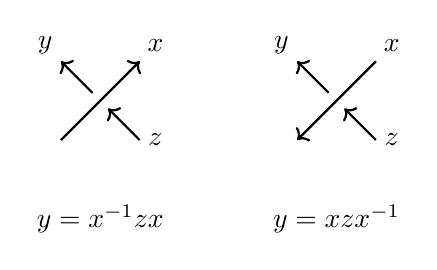
\begin{tikzpicture}
\draw[thick,->] (0,0)--(1,1);
\draw[thick,->] (1,0)--(0.6,0.4);
\draw[thick,->] (0.4,0.6)--(0,1);
\node at (1.2,1.2){$x$};
\node at (-0.2,1.2){$y$};
\node at (1.2,0){$z$};
\node at (0.5,-1){$y=x^{-1}zx$};

\draw[thick,->] (4,1)--(3,0);
\draw[thick,->] (4,0)--(3.6,0.4);
\draw[thick,->] (3.4,0.6)--(3,1);
\node at (4.2,1.2){$x$};
\node at (2.8,1.2){$y$};
\node at (4.2,0){$z$};
\node at (3.5,-1){$y=xzx^{-1}$};

\end{tikzpicture}
    \caption{Types of Crossings}
    \label{fig:wp}
\end{figure}
These generators and relators form a balanced presentation of the fundamental group of the knot complement. Moreover, there exists an ordering of the relators and a choice of $\pm 1$ as exponents such that the relators satisfy the equation
$$\prod_{i=1}^nr_i^{\pm1}=1.
$$
Thus any relator $r_k$ can be eliminated, giving $\langle x_1,\cdots,x_n\mid r_1,\cdots,r_{k-1},r_{k+1},\cdots,r_n\rangle$, without changing the underlying group. When the knot is an unknot, the fundamental group of the knot complement is $\mathbb{Z}$, which can be generated by any generator $x_i$. So after adding a relator $w$ which is any word in $x_1,\ldots,x_n$ with exponent sum $\pm1$, we get a balanced presentation $\langle x_1,\cdots,x_n\mid r_1,\cdots,r_{k-1},r_{k+1},\cdots,r_n,w\rangle$ of the trivial group as in \textbf{Proposition~\ref{prop:unknot}}.

\subsubsection{Reidemeister moves are stable Andrews-Curtis moves} Two diagrams of the same knot can be related by a finite sequence of the three
Reidemeister moves in Figure \ref{fig:rm}. Here we distinguish \textbf{R2a} and \textbf{R2b} just because they give slightly different computation about the presentations. First described in \cite{WADA1994241}, Reidemeister moves can be realized by (AC1)–(AC5). We list the correspondence between Reidemeister moves and (AC1)–(AC5) as follows for self-containment. We consider the presentations obtained from Wirtinger presentations of any unknot diagram by eliminating one arbitrary relator and adding one relator $w$ which is any word in the generators with exponent sum $\pm1$, as described in the previous subsection. Since we want to consider their behavior under Reidemeister moves, we can assume that the relator eliminated is not one given by the crossings in \textbf{R1}, \textbf{R2a}, \textbf{R2b}, \textbf{R3}. We note, however, that since any relator in a Wirtinger presentation can be written as the product of the other relators, the relator we eliminated can be recovered using (AC1)–(AC3).
\\
\\
\textbf{R1}:
\begin{align*}
\langle x_1,\cdots,x_n,x,y\mid r_1,\cdots,r_n,yx^{-1},w\rangle\longleftrightarrow\langle x_1,\cdots,x_n,x\mid r_1',\cdots,r_n',w'\rangle
\end{align*}
Here $r_i'$ and $w'$ are obtained from replacing $y$ in $r_i$ and $w$ by $x$. The equivalence comes from the substitution in \textbf{Lemma~\ref{lem:substitution}}.
\\
\\
\textbf{R2a}:
\begin{align*}
\,\,&\langle x_1,\cdots,x_n,x,y,z,u\mid r_1,\cdots,r_{n+1},xyz^{-1}y^{-1},zy^{-1}u^{-1}y,w\rangle
\\
&\longleftrightarrow\langle x_1,\cdots,x_n,x,y,u\mid r_1',\cdots,r_{n+1}',ux^{-1},w'\rangle
\\
&=\langle x_1,\cdots,x_n,x,y,u\mid r_1,\cdots,r_{n+1},ux^{-1},w'\rangle
\\
&\longleftrightarrow\langle x_1,\cdots,x_n,x,y\mid \tilde{r}_1,\cdots,\tilde{r}_{n+1},\tilde{w}\rangle
\end{align*}
Here $r_i',w'$ are obtained from replacing $z$ in $r_i,w$ by $y^{-1}xy$; $\tilde{r_i}$ from replacing $u$ in $r_i$ by $x$; and $\tilde{w}$ from replacing $u$ in $w'$ by $x$. The second equation comes from the fact that the $r_i$ do not contain $z$.
\\
\textbf{R2b} is similar to \textbf{R2a}.
\\
\\
\textbf{R3}:
\begin{align*}
&\langle x_1,\cdots,x_n,x,y,z,u,v,r\mid r_1,\cdots,r_{n+2},vxy^{-1}x^{-1},urv^{-1}r^{-1},rxz^{-1}x^{-1},w\rangle
\\
&\longleftrightarrow\langle x_1,\cdots,x_n,x,y,z,u,r\mid r_1,\cdots,r_{n+2},urxy^{-1}x^{-1}r^{-1},rxz^{-1}x^{-1},w'\rangle
\\
&\longleftrightarrow\langle x_1,\cdots,x_n,x,y,z,u,r\mid r_1,\cdots,r_{n+2},uxzy^{-1}z^{-1}x^{-1},rxz^{-1}x^{-1},w'\rangle
\\
&\longleftrightarrow\langle x_1,\cdots,x_n,x,y,z,u,r,t\mid r_1,\cdots,r_{n+2},uxzy^{-1}z^{-1}x^{-1},rxz^{-1}x^{-1},tzy^{-1}z^{-1},w'\rangle
\\
&\longleftrightarrow\langle x_1,\cdots,x_n,x,y,z,u,r,t\mid r_1,\cdots,r_{n+2},rxz^{-1}x^{-1},tzy^{-1}z^{-1},uxt^{-1}x^{-1},w'\rangle
\end{align*}
Here $w'$ is obtained from replacing $v$ in $w$ by $xyx^{-1}$.


After reducing our diagram to the trivial diagram of the unknot, we are left with $\langle x \mid \bar w\rangle$, where $\bar w$ is $w$ after applying all the Reidemeister moves. This is because the trivial diagram of the unknot gives the presentation $\langle x\mid \,\,\rangle$ of the infinite cyclic group, so $\bar w$ is the only relator remaining.  Moreover, $\bar w = x^{\pm1}$ since at each stage, $w$ has exponent sum $\pm 1$, so $\langle x \mid \bar w\rangle$ can be reduced to the trivial presentation $\langle \,\, \mid \,\, \rangle$. Thus \textbf{Proposition \ref{prop:unknot}} is proven.

\begin{figure}
    \centering
\begin{tikzpicture}
\draw[thick,rounded corners] (0,0)--(2,0)--(2,-1)--(1,-1)--(1,-0.2);
\draw[thick,rounded corners] (1,0.2)--(1,1);

\draw[<->] (2.5,0)--(3.5,0);

\draw[thick,rounded corners] (4,0)--(5,0)--(5,1);

\node at (4.5,-0.5){$x$};
\node at (0.5,-0.5){$x$};
\node at (1.5,0.5){$y$};

\node at (0.5,0){$>$};
\node at (1,0.5){\rotatebox{90}{$>$}};
\node at (4.5,0){$>$};

\node at (-0.5,0){\textbf{R1}};

\node at (7.5,-3){\textbf{R2b}};

\draw[thick] (9,-2)--(9,-2.3);
\draw[thick] (9,-2.7)--(9,-3.3);
\draw[thick] (9,-3.7)--(9,-4);

\draw[thick,rounded corners] (10,-2)--(10,-2.5)--(8.5,-2.5)--(8.5,-3.5)--(10,-3.5)--(10,-4);

\node at (9,-1.7){$x$};
\node at (10,-1.7){$y$};
\node at (9.2,-3){$z$};
\node at (9,-4.3){$u$};

\node at (9,-2){\rotatebox{90}{$>$}};
\node at (10,-2){\rotatebox{90}{$>$}};
\node at (9,-3){\rotatebox{90}{$>$}};
\node at (9,-3.7){\rotatebox{90}{$>$}};

\draw[<->] (10.5,-3)--(11.5,-3);

\draw[thick] (12.5,-2)--(12.5,-4);
\draw[thick] (13.5,-2)--(13.5,-4);

\node at (12.5,-3){\rotatebox{90}{$>$}};
\node at (13.5,-3){\rotatebox{90}{$>$}};

\node at (12.5,-1.7){$x$};
\node at (13.5,-1.7){$y$};

\draw[thick] (1,-2)--(1,-2.3);
\draw[thick] (1,-2.7)--(1,-3.3);
\draw[thick] (1,-3.7)--(1,-4);

\draw[thick,rounded corners] (2,-2)--(2,-2.5)--(0.5,-2.5)--(0.5,-3.5)--(2,-3.5)--(2,-4);

\node at (1,-2){\rotatebox{90}{$>$}};
\node at (2,-2.3){\rotatebox{90}{$<$}};
\node at (1,-3){\rotatebox{90}{$>$}};
\node at (1,-3.7){\rotatebox{90}{$>$}};

\draw[<->] (2.5,-3)--(3.5,-3);

\draw[thick] (4.5,-2)--(4.5,-4);
\draw[thick] (5.5,-2)--(5.5,-4);

\node at (4.5,-3){\rotatebox{90}{$>$}};
\node at (5.5,-3){\rotatebox{90}{$<$}};

\node at (4.5,-1.7){$x$};
\node at (5.5,-1.7){$y$};

\node at (1,-1.7){$x$};
\node at (2,-1.7){$y$};
\node at (1.2,-3){$z$};
\node at (1,-4.3){$u$};

\node at (-0.5,-3){\textbf{R2a}};

\draw[thick] (1,-5)--(1,-8);
\draw[thick] (0.5,-7.5)--(0.8,-7.5);
\draw[thick,rounded corners] (1.2,-7.5)--(2,-7.5)--(2,-5.5)--(3.5,-5.5);
\draw[thick] (0.5,-6.5)--(0.8,-6.5);
\draw[thick] (1.2,-6.5)--(1.8,-6.5);
\draw[thick] (2.2,-6.5)--(3.5,-6.5);

\draw[<->] (4,-6.5)--(5,-6.5);

\draw[thick] (5.5,-6.5)--(6.8,-6.5);
\draw[thick,rounded corners] (5.5,-7.5)--(7,-7.5)--(7,-5.5)--(7.8,-5.5);
\draw[thick,rounded corners] (7.2,-6.5)--(7.8,-6.5);
\draw[thick] (8,-5)--(8,-8);
\draw[thick] (8.2,-5.5)--(8.5,-5.5);
\draw[thick] (8.2,-6.5)--(8.5,-6.5);

\node at (0.5,-5.5){$x$};
\node at (0.5,-6.2){$y$};
\node at (0.5,-7.2){$z$};
\node at (3,-5.2){$r$};
\node at (3,-6.2){$u$};
\node at (1.5,-6.2){$v$};

\node at (1,-5.5){\rotatebox{90}{$>$}};
\node at (0.7,-6.5){$>$};
\node at (0.7,-7.5){$>$};
\node at (1.5,-6.5){$>$};
\node at (3,-5.5){$>$};
\node at (3,-6.5){$>$};

\node at (8,-4.5){$x$};
\node at (6,-6.2){$y$};
\node at (6,-7.2){$z$};
\node at (9,-5.5){$r$};
\node at (9,-6.5){$u$};
\node at (7.5,-6.2){$t$};

\node at (8,-5){\rotatebox{90}{$>$}};
\node at (6,-6.5){$>$};
\node at (6,-7.5){$>$};
\node at (8.5,-6.5){$>$};
\node at (8.5,-5.5){$>$};
\node at (7.5,-6.5){$>$};

\node at (-0.5,-6){\textbf{R3}};

\end{tikzpicture}
    \caption{Reidemeister moves}
    \label{fig:rm}
\end{figure}


\subsubsection{Constructing Infinite Familes}
Any diagram of the unknot with $n$ crossings gives us $n$ examples of infinite families of presentations that are known to be stably AC-trivial, as given by the proposition.

Moreover, we can use stable AC-moves, especially the substitution move in Lemma~\ref{lem:substitution}, to reduce the number of generators and relations in these families of presentations. Indeed, if we restrict our attention to the relators coming from the Wirtinger presentation (i.e., without changing the free choice of $w$), we can get similar infinite families of presentations with fewer generators. This is valuable since most of the focus in studying the (stable) Andrews-Curtis conjecture is given to presentations with a small number of generators, especially 2 and 3.

\begin{remark}
This approach can at best generate interesting infinite families with three generators and relators, since removing $w$ will always give us a presentation of $\mathbb{Z}$ and so any two-generator presentation must be just $\langle x,y \mid x=\pm y, w\rangle$.
\end{remark}
\begin{remark}
    Each infinite family coming from Proposition~\ref{prop:unknot} will give many distinct infinite families with fewer generators, as we have many different ways to simplify the groups that lead to different presentations.
\end{remark}
\begin{remark}
    In order to get interesting examples, it seems sensible to look at hard unknot diagrams, as the easier it is to change the diagram into the trivial diagram of the unknot, the easier it should be for the computer algorithms to trivialize the resulting presentations.
\end{remark}
\begin{remark}
    On the other hand, the more complicated the knot diagram, the harder it will be to simplify the presentation down to three generators, and the less likely such a presentation is of reasonable length.
\end{remark}
\begin{remark}
    We can also make presentations more complicated by choosing simplification steps that make the presentation more complicated. However it seems more likely to get interesting presentations from choosing a complicated knot diagram and simplifying more.
\end{remark}

\begin{conjecture}
    Every stably AC-trivial presentation of the form from Proposition~\ref{prop:unknot} can also be stably AC-trivialized without (AC4), and in particular by just doing substitutions.
\end{conjecture}

Note that realizing Reidemeister moves with stable AC moves \emph{does} require (AC4), and thus this conjecture is not a consequence of the proof of the proposition. We checked that it holds in many of hard unknot diagrams in \cite{burton2021harddiagramsunknot}, in particular for the Culprit, D28, Goeritz, Ochai I, and Tuzun Sikora.

If true, it provides some evidence against this approach generating lots of interesting examples of stably AC-trivial presentations.
\subsubsection{Examples}
One famous hard unknot diagram is the Culprit, first introduced in \cite{kauffman2014hardunknotscollapsingtangles}, which has 10 crossings . One possibly interesting infinite family coming from this diagram is the following:
\begin{proposition}
    Any presentation of the form
    \[
\langle x,y,z \,\mid \, xzxz^{-1}x^{-1}yzyz^{-1}y^{-1}z^{-1}y^{-1}, zx^{-1}yzy^{-1}z^{-1}y^{-1}x, w \rangle,
\] where $w$ is a word with exponent sum $\pm 1$, is a stably AC-trivial presentation of the trivial group. [is it worth showing the substitution steps of how you get this presentation from the culprit?]
\end{proposition}
However, it is difficult to find a choice of $w$ that gives any non-trivial result. For example, if $w=z^{-1}w'$, where $w'$ is a word in $x$ and $y$ of length $\leq 8$, then the greedy search is able to instantly trivialize the presentation.
	\appendix
	% !TEX root = ../ac_paper.tex

\section{Hyperparameters}\label{app:hyperparameters}

Here we discuss the hyperparameters used to train the Proximal Policy Optimization (PPO) and Transformer models of \autoref{sec:rl} and \autoref{sec:lm} respectively.
The hyperparameters of PPO are given in \autoref{tab:ppo_hyperparameters}. These hyperparameters were defined in the main text in \autoref{sec:ppo}. Each of the two networks --- the actor and the critic --- was a 2-layer feed forward neural network with 512 neurons and $tanh$ non-linearlities. We used Adam optimizer for training.


The performance of PPO is known to be highly sensitive to various implementation details in addition to the choice of hyperparameters \cite{shengyi2022the37implementation, engstrom2020implementation}. We used the single-file implementation of PPO in CleanRL \cite{huang2022cleanrl}, which has been well-benchmarked against the results of the original paper \cite{schulman2017proximal}. Following  \cite{engstrom2020implementation}, we used advantage normalization and clipped value loss. If the KL divergence between the old and the updated policy exceeded the target KL divergence in a mini-batch, we skipped the remaining mini-batches in the optimization phase to avoid a large jump in policy.
We did not ablate all of the choices of hyperparameters to investigate the importance of each choice.

\begin{table}[ht]
    \centering
    \begin{tabular}{lc}
        \hline
        Hyperparameter & Value \\
        \hline
        Horizon $(T)$ & 200 \\
        Rollout Length $(T')$ & 200 \\
        Number of parallel actors & 28 \\
        Total Number of Rollouts & $\sim 2 \times 10^5$ \\
        Maximum Learning Rate & $1.0 \times 10^{-4}$ \\
        Minimum Learning Rate & 0 \\
        Learning Rate Schedule & Linear Decay \\
        Number of epochs & 1 \\
        Number of mini-batches & 4 \\
        Optimization mini-batch size & 1400 \\
        Discount ($\gamma$) & 0.999 \\
        GAE parameter ($\lambda$) & 0.95 \\
        Clipping parameter $\epsilon$ & 0.2 \\
        Value Loss coefficient, $c_1$ & 0.5 \\
        Entropy Loss coefficient, $c_2$ & 0.01 \\
        Adam epsilon parameter & $10^{-5}$ \\
        Target KL divergence & 0.01 \\
        \hline
    \end{tabular}
    \caption{Table of Hyperparameters}
    \label{tab:ppo_hyperparameters}
\end{table}

The Transformer model studied in \autoref{sec:lm} is an 8-layer transformer model with the embedding space dimension of $512$ and $4$ attention heads. The context window of the Transformer had length $1024$. We used a batch size of $12$ and constant learning rate of $6 \times 10^{-5}$. We trained for a total of $25000$ iterations. We used AdamW optimizer for training with hyperparameters $\beta_1 = 0.9$ and $\beta_2 = 0.99$. We did not use any dropout during training.
        \todo{Add details on choices of hyperparameters in the experiments for scaling trends of Section 5.}
        \todo{Comment that normalizing rewards through a running estimate instead of rescaling rewards helps improve performance. Also mention the order of clipping and normalizing rewards. In the equation in section 4.3, we clip rewards, but it helps to normalize first and then clip.}
        % !TEX root = ../ac_paper.tex

\section{RL path \label{app:RLpath}}

\[
\begin{aligned}
& h_{2} \cdot h_{8} \cdot h_{6} \cdot h_{4} \cdot h_{10} \cdot h_{2} \cdot h_{8} \cdot h_{6} \cdot h_{6} \cdot h_{8} \cdot h_{10} \cdot h_{10} \cdot h_{10} \cdot h_{7} \cdot h_{0} \cdot h_{4} \cdot h_{6} \cdot h_{6} \\ &
h_{6} \cdot h_{6} \cdot h_{11} \cdot h_{8} \cdot h_{10} \cdot h_{10} \cdot h_{2} \cdot h_{8} \cdot h_{6} \cdot h_{4} \cdot h_{10} \cdot h_{2} \cdot h_{8} \cdot h_{6} \cdot h_{6} \cdot h_{6} \cdot h_{8} \cdot h_{10} \\ &
h_{10} \cdot h_{10} \cdot h_{7} \cdot h_{3} \cdot h_{5} \cdot h_{5} \cdot h_{5} \cdot h_{0} \cdot h_{4} \cdot h_{6} \cdot h_{11} \cdot h_{5} \cdot h_{9} \cdot h_{7} \cdot h_{11} \cdot h_{7} \cdot h_{11} \cdot h_{5} \\ &
h_{4} \cdot h_{9} \cdot h_{2} \cdot h_{8} \cdot h_{6} \cdot h_{6} \cdot h_{6} \cdot h_{8} \cdot h_{10} \cdot h_{8} \cdot h_{10} \cdot h_{10} \cdot h_{4} \cdot h_{7} \cdot h_{0} \cdot h_{4} \cdot h_{6} \cdot h_{11} \\ &
h_{2} \cdot h_{8} \cdot h_{6} \cdot h_{6} \cdot h_{8} \cdot h_{10} \cdot h_{8} \cdot h_{10} \cdot h_{2} \cdot h_{8} \cdot h_{4} \cdot h_{10} \cdot h_{7} \cdot h_{0} \cdot h_{4} \cdot h_{6} \cdot h_{4} \cdot h_{11} \\ &
h_{10} \cdot h_{2} \cdot h_{8} \cdot h_{6} \cdot h_{4} \cdot h_{10} \cdot h_{8} \cdot h_{7} \cdot h_{0} \cdot h_{4} \cdot h_{6} \cdot h_{11} \cdot h_{4} \cdot h_{7} \cdot h_{11} \cdot h_{2} \cdot h_{8} \cdot h_{6} \\ &
h_{2} \cdot h_{8} \cdot h_{6} \cdot h_{8} \cdot h_{8} \cdot h_{10} \cdot h_{7} \cdot h_{0} \cdot h_{4} \cdot h_{0} \cdot h_{4} \cdot h_{0} \cdot h_{4} \cdot h_{0} \cdot h_{4} \cdot h_{6} \cdot h_{11} \cdot h_{2} \\ &
h_{8} \cdot h_{6} \cdot h_{4} \cdot h_{6} \cdot h_{8} \cdot h_{8} \cdot h_{10} \cdot h_{10} \cdot h_{10} \cdot h_{10} \cdot h_{2} \cdot h_{8} \cdot h_{6} \cdot h_{4} \cdot h_{10} \cdot h_{8} \cdot h_{7} \cdot h_{0} \\ &
h_{4} \cdot h_{6} \cdot h_{11} \cdot h_{4} \cdot h_{2} \cdot h_{8} \cdot h_{6} \cdot h_{6} \cdot h_{8} \cdot h_{8} \cdot h_{10} \cdot h_{10} \cdot h_{7} \cdot h_{0} \cdot h_{4} \cdot h_{0} \cdot h_{4} \cdot h_{6} \\ &
h_{11} \cdot h_{8} \cdot h_{7} \cdot h_{11} \cdot h_{5} \cdot h_{4} \cdot h_{8} \cdot h_{11} \cdot h_{7} \cdot h_{4} \cdot h_{8} \cdot h_{11} \cdot h_{7} \cdot h_{9} \cdot h_{6} \cdot h_{8} \cdot h_{8} \cdot h_{10} \\ &
h_{4} \cdot h_{10} \cdot h_{10} \cdot h_{8} \cdot h_{2} \cdot h_{8} \cdot h_{6} \cdot h_{7} \cdot h_{8} \cdot h_{11} \cdot h_{8} \cdot h_{10} \cdot h_{4} \cdot h_{10} \cdot h_{10} \cdot h_{2} \cdot h_{8} \cdot h_{6} \\ &
h_{4} \cdot h_{6} \cdot h_{8} \cdot h_{8} \cdot h_{8} \cdot h_{10} \cdot h_{7} \cdot h_{11} \cdot h_{7} \cdot h_{4} \cdot h_{11} \cdot h_{10} \cdot h_{7} \cdot h_{0} \cdot h_{4} \cdot h_{6} \cdot h_{11} \cdot h_{4} \\ &
h_{2} \cdot h_{8} \cdot h_{6} \cdot h_{8} \cdot h_{8} \cdot h_{8} \cdot h_{10} \cdot h_{7} \cdot h_{0} \cdot h_{4} \cdot h_{0} \cdot h_{4} \cdot h_{0} \cdot h_{4} \cdot h_{6} \cdot h_{8} \cdot h_{11} \cdot h_{2} \\ &
h_{8} \cdot h_{8} \cdot h_{10} \cdot h_{10} \cdot h_{10} \cdot h_{2} \cdot h_{8} \cdot h_{2} \cdot h_{8} \cdot h_{6} \cdot h_{4} \cdot h_{6} \cdot h_{8} \cdot h_{10} \cdot h_{8} \cdot h_{10} \cdot h_{10} \cdot h_{7} \\ &
h_{0} \cdot h_{4} \cdot h_{6} \cdot h_{11} \cdot h_{4} \cdot h_{2} \cdot h_{8} \cdot h_{6} \cdot h_{4} \cdot h_{2} \cdot h_{8} \cdot h_{6} \cdot h_{8} \cdot h_{10} \cdot h_{7} \cdot h_{11} \cdot h_{7} \cdot h_{5} \\ &
h_{11} \cdot h_{8} \cdot h_{10} \cdot h_{4} \cdot h_{8} \cdot h_{9} \cdot h_{7} \cdot h_{4} \cdot h_{8} \cdot h_{9} \cdot h_{7} \cdot h_{0} \cdot h_{4} \cdot h_{0} \cdot h_{4} \cdot h_{6} \cdot h_{11} \cdot h_{5} \\ &
h_{9} \cdot h_{4} \cdot h_{2} \cdot h_{8} \cdot h_{6} \cdot h_{4} \cdot h_{6} \cdot h_{8} \cdot h_{8} \cdot h_{10} \cdot h_{10} \cdot h_{7} \cdot h_{0} \cdot h_{4} \cdot h_{6} \cdot h_{11} \cdot h_{6} \cdot h_{8} \\ &
h_{8} \cdot h_{10} \cdot h_{4} \cdot h_{10} \cdot h_{2} \cdot h_{8} \cdot h_{6} \cdot h_{8} \cdot h_{8} \cdot h_{10} \cdot h_{7} \cdot h_{11} \cdot h_{7} \cdot h_{5} \cdot h_{11} \cdot h_{9} \cdot h_{7} \cdot h_{9} \\ &
h_{7} \cdot h_{4} \cdot h_{0} \cdot h_{4} \cdot h_{6} \cdot h_{11} \cdot h_{8} \cdot h_{8} \cdot h_{8} \cdot h_{10} \cdot h_{7} \cdot h_{0} \cdot h_{4} \cdot h_{6} \cdot h_{4} \cdot h_{11} \cdot h_{10} \cdot h_{2} \\ &
h_{8} \cdot h_{8} \cdot h_{8} \cdot h_{10} \cdot h_{7} \cdot h_{0} \cdot h_{4} \cdot h_{6} \cdot h_{11} \cdot h_{4} \cdot h_{2} \cdot h_{8} \cdot h_{8} \cdot h_{2} \cdot h_{8} \cdot h_{10} \cdot h_{2} \cdot h_{8} \\ &
h_{6} \cdot h_{4} \cdot h_{6} \cdot h_{8} \cdot h_{10} \cdot h_{7} \cdot h_{0} \cdot h_{4} \cdot h_{6} \cdot h_{11} \cdot h_{8} \cdot h_{8} \cdot h_{8} \cdot h_{8} \cdot h_{8} \cdot h_{8} \cdot h_{8} \cdot h_{1} \\ &
h_{7} \cdot h_{5} \cdot h_{11}
\end{aligned}
\]
	% !TEX root = ../ac_paper.tex

\section{Construction of neighborhoods}\label{s:neighborhoods}

\subsection{Neighborhoods for MS series}

We define the $n$-neighborhood of a balanced presentation $\pi$ as the set of all balanced presentations that can be obtained by applying at most $n$ AC-moves to $\pi$.
We used Algorithm \ref{alg:bfs_neigh}, a variation of the Breadth-First Search (BFS) algorithm, to generate $5$-neighborhoods of presentations in the Miller–Schupp series.
We did this in two settings: in the first, we considered the presentation as a tuple of relators (meaning that the order of relators is important), and in the second, we considered the presentation as a set of relators (meaning that the order of relators is not important; implemented as a tuple of relators in lexicographic order).

\subsection{Neighborhoods of the identity} For any $\ell \in \{3, \dots, 14\}$, we constructed a neighborhood of the identity using the same BFS algorithm. This neighborhood contains all presentations that can be connected to the identity via a path of AC moves, where each presentation in the path has a length less than or equal to $\ell$.

\begin{algorithm}
	\caption{Breadth-First Search Algorithm Bounded by Size}\label{alg:bfs_1}
	\begin{algorithmic}[1]
		\State \textbf{Input:} A balanced presentation $\pi$, maximal size of presentation $n$
		\State \textbf{Output:} Set of enumerated presentations connected to the starting presentation that are achievable without exceeding the size limit, and set of edges with filtrations
		\State Initialize a queue $Q$, set of visited nodes $visited$, and numerical map $name$ that will enumerate presentations
		\State Mark $\pi$ as visited, put it into queue $Q$, and assign it the number $0$
		\While{$Q$ is not empty}
		\State $u \gets $ top of $Q$ \Comment{Remove the front node of $Q$}
		\For{every AC move $m$}
		\State $child \gets m(u)$
		\If{$child$'s size $\leq n$ and $child$ is not visited}
		\State Put $child$ in $Q$ and mark it as visited
		\State Assign $child$ the next available number
		\EndIf
		\If{$child$'s size $\leq n$ and $u$'s number is smaller than $child$'s number}
		\State Return edge $(u, child)$ with proper filtration
		\EndIf
		\EndFor
		\EndWhile
	\end{algorithmic}
\end{algorithm}

\begin{algorithm}
	\caption{Breadth-First Search Algorithm Bounded by Number of Steps}\label{alg:bfs_neigh}
	\begin{algorithmic}[1]
		\State \textbf{Input:} A balanced presentation $\pi$, positive integer $n$
		\State \textbf{Output:} $n$-neighborhood of $\pi$
		\State Initialize a queue $Q$, set of visited nodes $visited$, and numerical map $dist$ that represents the minimal number of AC-moves needed to transform $\pi$ into a given presentation
		\State Mark $\pi$ as visited, put it into queue $Q$, and set its distance to $0$
		\While{$Q$ is not empty}
		\State $u \gets $ top of $Q$ \Comment{Remove the front node of $Q$}
		\For{every AC move $m$}
		\State $child \gets m(u)$
		\If{$dist[u] < n$ and $child$ is not in $visited$}
		\State Put $child$ in $Q$ and mark it as visited
		\State Set $dist[child] := dist[u] + 1$
		\EndIf
		\EndFor
		\EndWhile
		\Return set $visited$
	\end{algorithmic}
\end{algorithm}
	% !TEX root = ../ac_paper.tex

\section{Language Modeling Dataset Generation \label{app:algorithm}}

This appendix describes the method, \autoref{alg:apply_ac_moves}, used to generate the training and evaluation datasets for the Transformer model, as referenced in \autoref{sec:lm}. Our aim was to create datasets featuring presentations of varying lengths. We began with a presentation \(P_0\) from the Miller--Schupp series, where \(n, \length(w) \leq 7\), setting a maximum relator length \(l_{\text{max}} = 128\). Presentations were generated in \(n=128\) phases, each phase allowing a maximum relator length \(l_i \sim \mathcal{U}(l + i \cdot l_{\text{inc}}, l + (i+1) \cdot l_{\text{inc}})\). Here, \(l\) represents the longest relator length in \(P_0\) and \(l_{\text{inc}} = (l_{\text{max}} - l)/n\) is the incremental increase per phase. In each phase, we selected a presentation \(P\) from the previous phase and applied \(N=1000\) AC$'$ moves. Any AC$'$ move that exceeded the length \(l_i\) resulted in no change.


We repeated this for all 1190 presentations in the Miller--Schupp series, ultimately producing approximately 1.8 million balanced presentations. The length distribution of these presentations is detailed in \autoref{fig:gpt_data}.

\begin{algorithm}
    \caption{Transformer Dataset Generation}
    \label{alg:apply_ac_moves}
    \begin{algorithmic}[1]
        \State \textbf{Input:}
     	\begin{itemize}
	\item[]     $P_0$  --- an initial presentation with $l$ as the length of the longest relator
          \item[]   $n$  --- number of phases
           \item[]  $m$  --- number of presentations in each phase
           \item[]  $N$  --- number of AC$'$ moves to apply in each phase
         \item[]    $l_{\text{max}}$  --- upper bound on presentation lengths in the dataset
          \end{itemize}
         \State \textbf{Output:}
         \begin{itemize}
         \item[]         Dataset (the final collection of presentations)
         \end{itemize}
        \State Dataset $\gets \emptyset$ \Comment{Initialize the dataset of all presentations}
        \State $l_{\text{inc}} \gets (l_{\text{max}} - l) / n$ \Comment{Increment for the maximum relator length per phase}
        \For{$i = 0$ \textbf{to} $n-1$} \Comment{Loop over each phase}
            \For{$j = 1$ \textbf{to} $m$} \Comment{Generate $m$ presentations for each phase}
                \State $l_i \sim \mathcal{U}(l + i \cdot l_{\text{inc}}, l + (i+1) \cdot l_{\text{inc}})$
                \Comment{Sample maximum relator length}
		\State $P \gets (i = 1) \ ? \ P_0 \ : \ \text{Dataset}[(i-1) \cdot m + j - 1]$
                \For{$k = 1$ \textbf{to} $N$} \Comment{Apply $N$ AC$'$ moves with relator length $l_i$}
                    \State $A \sim \text{AC}' \text{ Moves}$
                    \State $P \gets A \cdot P$
                \EndFor
                \State Dataset $\gets$ Dataset $\cup \{P\}$
                \Comment{Add the presentation $P$ to the Dataset}
            \EndFor
        \EndFor
    \end{algorithmic}
\end{algorithm}
	% !TEX root = ../ac_paper.tex

\subsection*{Funding}

The work of A.S. is supported by the US Department of Energy grant DE-SC0010008 to Rutgers University. The authors acknowledge the contributions of Office of Advanced Research Computing (OARC) at Rutgers University for providing access to the Amarel cluster and other computing resources.
A.M.'s work is supported by NSERC grants RES000678 and R7444A03. A.M. also gratefully acknowledges the excellent working conditions provided by the Max Planck Institute for Mathematics in Bonn.
The work of P.K. and B.L. is supported by the SONATA grant no. 2022/47/D/ST2/02058 funded by the Polish National Science Centre. This research was carried out with the support of the Interdisciplinary Centre for Mathematical and Computational Modelling at the University of Warsaw (ICM UW).
The work of S.G. is supported in part by a Simons Collaboration Grant on New Structures in Low-Dimensional Topology, by the NSF grant DMS-2245099, and by the U.S. Department of Energy, Office of Science, Office of High Energy Physics, under Award No. DE-SC0011632.
Z.W. is partially supported by ARO MURI contract W911NF-20-1-0082. Y.Q. thanks Nankai Zhide Foundation for support.
	\sloppy
	\printbibliography
    
% !TEX root = ../ac_paper.tex

\section{Stable AC-trivialization of $\AK(3)$}\label{sec:stable_ak3}

Here we provide a sequence of AC transformations that relates the length-25 stably AC-trivial example of \cite{MMS}, 
\[
\angles{x, y \mid xyx^{-2}y^{-1} xy^{-1}, x^{-1} y^{-1} x y^2 x y^{-1}}.
\]
to $\AK(3)$. We discovered this sequence of transformations using the greedy search algorithm of \autoref{sec:search}. The reader may confirm with the help of a computer program or by hand that this sequence relates the two presentations. To describe the sequence, let us first recall the definitions of AC$'$ moves discussed in \autoref{sec:search},
\begin{enumerate}[label=(AC$'$\arabic*)]
	\item Substitute some $r_i$ by $r_i r_j^{\pm 1}$ for $i \neq j$.
	\item Change some $r_i$ to $g r_i g^{-1}$ where $g$ is a generator or its inverse.
\end{enumerate}

These are 12 transformations, which may be listed as follows.
\[
\begin{aligned}
h_1 &:= \  r_2 \rightarrow r_2 r_1 \\
h_2 &:= \ r_1 \rightarrow r_1 r_2^{-1} \\
h_3 &:= \ r_2 \rightarrow r_2 r_1^{-1} \\
h_4 &:= \ r_1 \rightarrow r_1 r_2 \\
h_5 &:= \ r_2 \rightarrow x^{-1} r_2 x \\
h_6 &:= \ r_1 \rightarrow y^{-1} r_1 y \\
h_7 &:= \ r_2 \rightarrow y^{-1} r_2 y \\
h_8 &:= \ r_1 \rightarrow x r_1 x^{-1} \\
h_9 &:= \ r_2 \rightarrow x r_2 x^{-1} \\
h_{10} &:= \ r_1 \rightarrow y r_1 y^{-1} \\
h_{11} &:= \ r_2 \rightarrow y r_2 y^{-1} \\
h_{12} &:= \ r_1 \rightarrow x^{-1} r_1 x 
\end{aligned}
\]

The sequence of moves that connects the length-25 presentation to $\AK(3)$ is as follows. 
\[
\begin{aligned}
& h_9 \cdot h_7 \cdot h_4 \cdot h_8 \cdot h_{11} \cdot h_5 \cdot h_{11} \cdot h_9 \cdot h_3 \cdot h_{10} \cdot h_{12} \cdot h_7 \cdot h_7 \cdot h_9 \cdot h_{11} \cdot h_5 \cdot h_3 \cdot h_5 \cdot \\
& h_4 \cdot h_3 \cdot h_{12} \cdot h_5 \cdot h_7 \cdot h_7 \cdot h_1 \cdot h_9 \cdot h_{11} \cdot h_8 \cdot h_3 \cdot h_5 \cdot h_{10} \cdot h_2 \cdot h_6 \cdot h_{12} \cdot h_9 \cdot h_7 \cdot \\
& h_5 \cdot h_{11} \cdot h_{10} \cdot h_3 \cdot h_8 \cdot h_{11} \cdot h_9 \cdot h_2 \cdot h_{10} \cdot h_{12} \cdot h_5 \cdot h_7 \cdot h_9 \cdot h_{11} \cdot h_1 \cdot h_9 \cdot h_8
\end{aligned}
\]
This sequence should be read from left to right; first apply $h_9$, then $h_7$, and so forth. This follows the standard convention of many programming languages, which iterate over lists from left to right by default. The total length of the presentation did not exceed $25$ during its path to $\AK(3)$. Additionally, we have not verified if this is the shortest path between the two presentations.



%\[
%\begin{array}{cc}
%[(9, 25), (7, 25), (4, 17), (8, 17), (11, 17), (5, 17), (11, 17), (9, 17), (3, 16), (10, 16), \\
 %(12, 16), (7, 16), (7, 16), (9, 16), (11, 16), (5, 16), (3, 15), (5, 15), (4, 19), (3, 14), (12, 14), \\
 %(5, 14), (7, 16), (7, 18), (1, 19), (9, 19), (11, 19), (8, 19), (3, 18), (5, 18), (10, 18), (2, 15), (6, 15), \\
 %(12, 15), (9, 15), (7, 15), (5, 15), (11, 15), (10, 15), (3, 15), (8, 15), (11, 15), (9, 15), (2, 16),\\
  %(10, 16), (12, 16), (5, 16), (7, 16), (9, 16), (11, 16), (1, 13), (9, 13), (8, 13)]
%\end{array}
%\]


    \todos
\end{document}